\documentclass{article}
\usepackage[utf8]{inputenc}
\usepackage{graphicx}
\usepackage{caption}
\usepackage{subcaption}
\usepackage{amsmath}


\title{Image and Video Processing Lab 5}
\author{Philine Witzig}
\date{December 2020}

\begin{document}

\maketitle

%---------------------------
% Task 1
%---------------------------
\section{Anchor Generation}

In this exercise, we were asked to perform image compression using JPEG for as many Q values as possible (multiple of $5$) and store the reconstructed results. For each of the three test images, compressed versions were created with a quality value for each $Q_i \in \{10, \dots, 90, 100 \}$. Figure \ref{fig:jpeg} shows the reconstructed versions for $Q=10, Q=60, Q=90$ for all three test images, as well as the original version. The above Q-values were chosen for the following reasons: For $Q=10$, i.e. the lowest compression level chosen, we obtain the strongest compression artefacts after reconstruction, including false contours and aliasing effects. These artefacts decrease with increasing Q value. For $Q=60$, the reconstructed version looks identical to the original version. Any higher Q-value will not lead to further improvement which can be observed for the $Q=90$ version. Furthermore, the bits per pixel (bpp) values for the above Q values are reported in Table \ref{tab:jpeg_bpp}.
\begin{figure}
    \centering
    \begin{subfigure}[b]{0.49 \textwidth}
    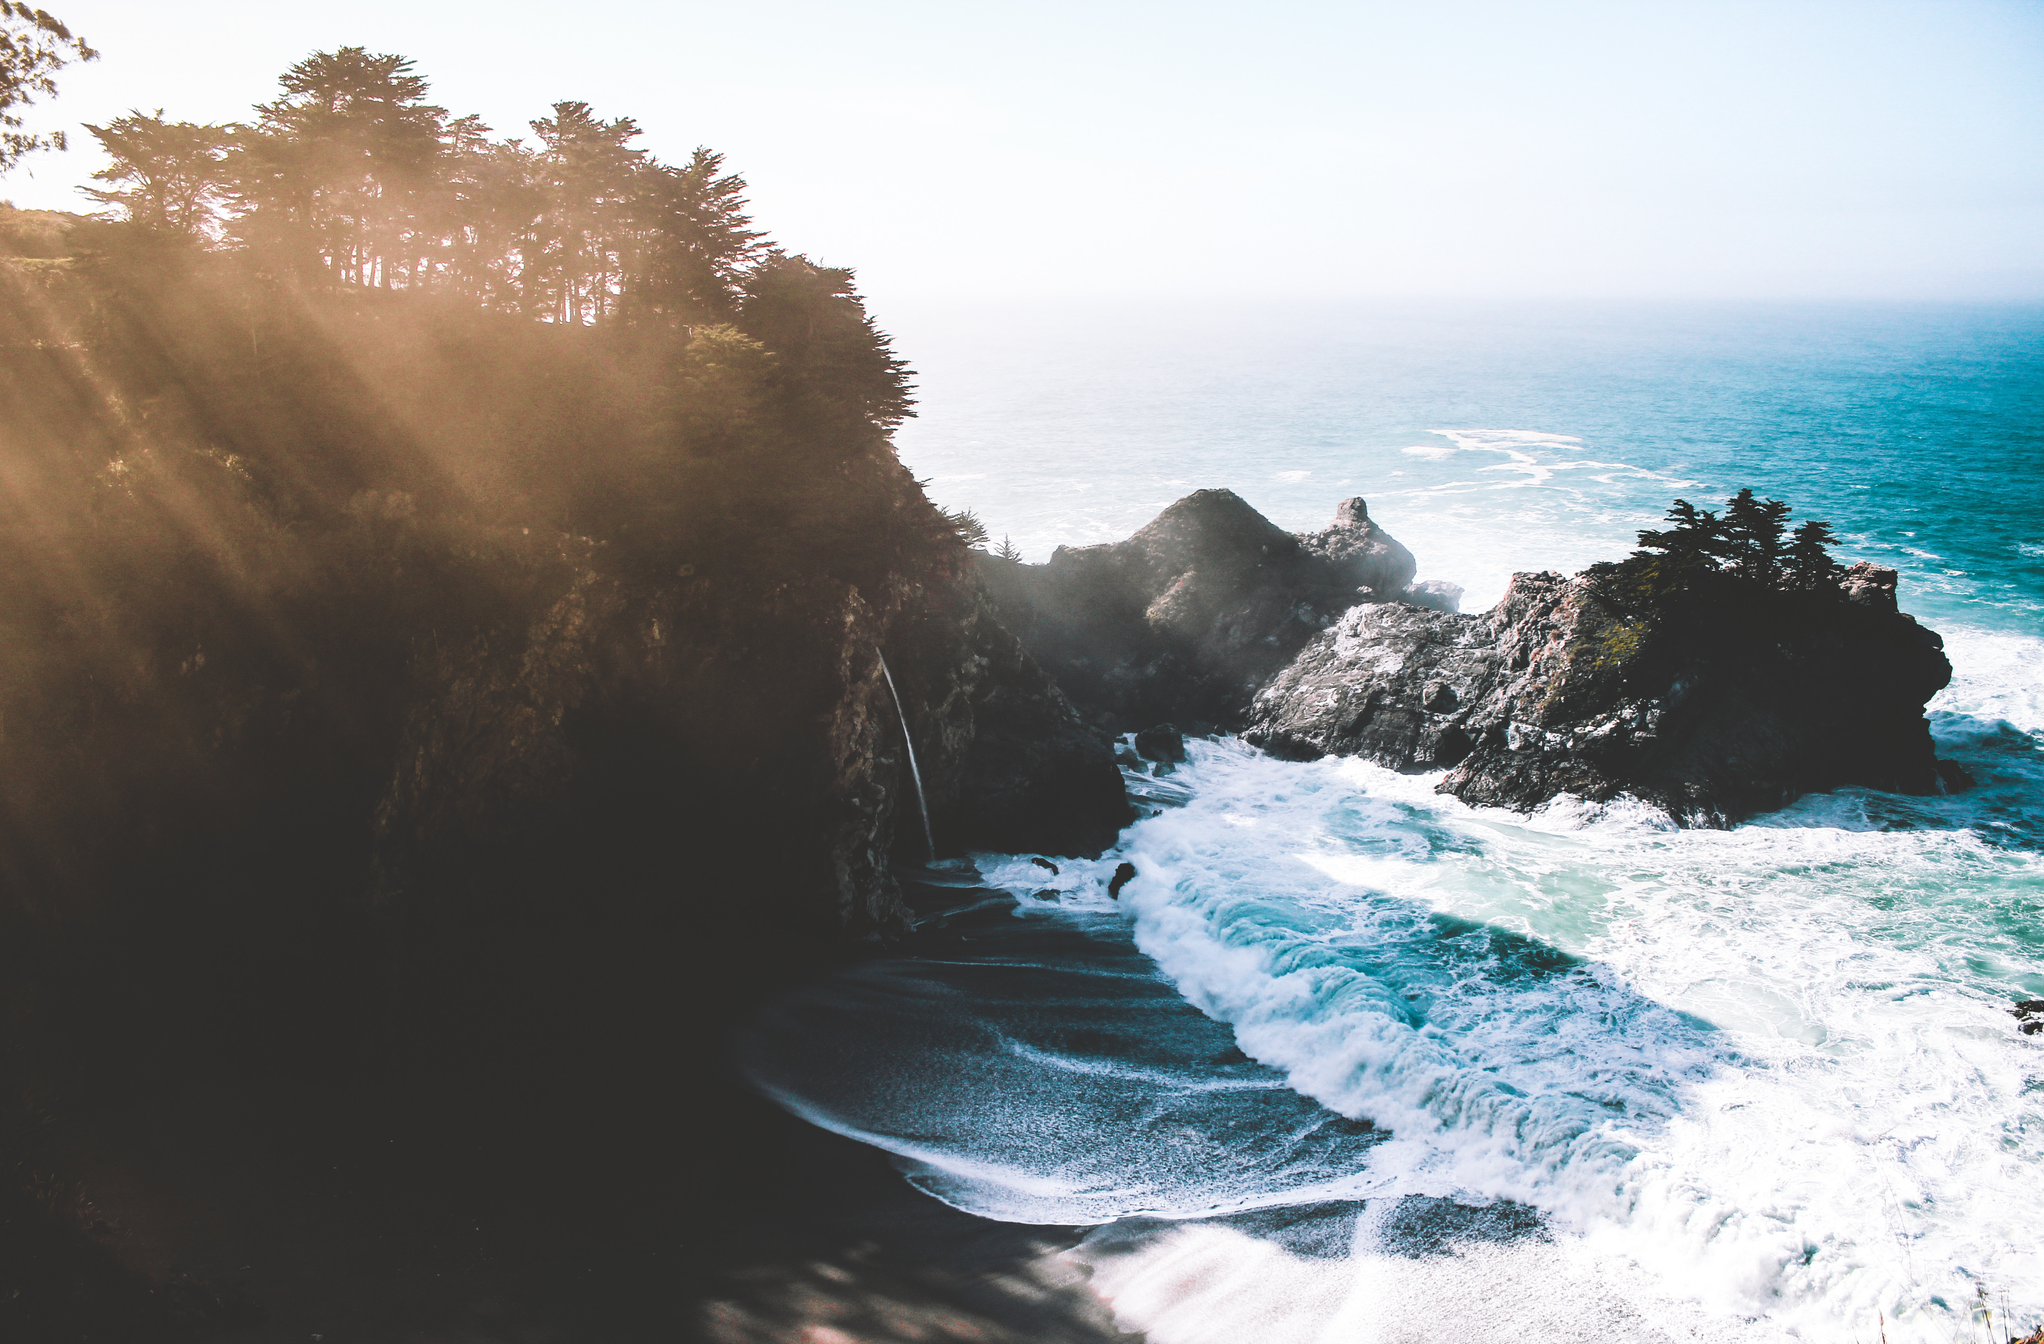
\includegraphics[width=\textwidth]{Images/test1.png}
    \subcaption{Original}
    \end{subfigure}
    \begin{subfigure}[b]{0.49 \textwidth}
    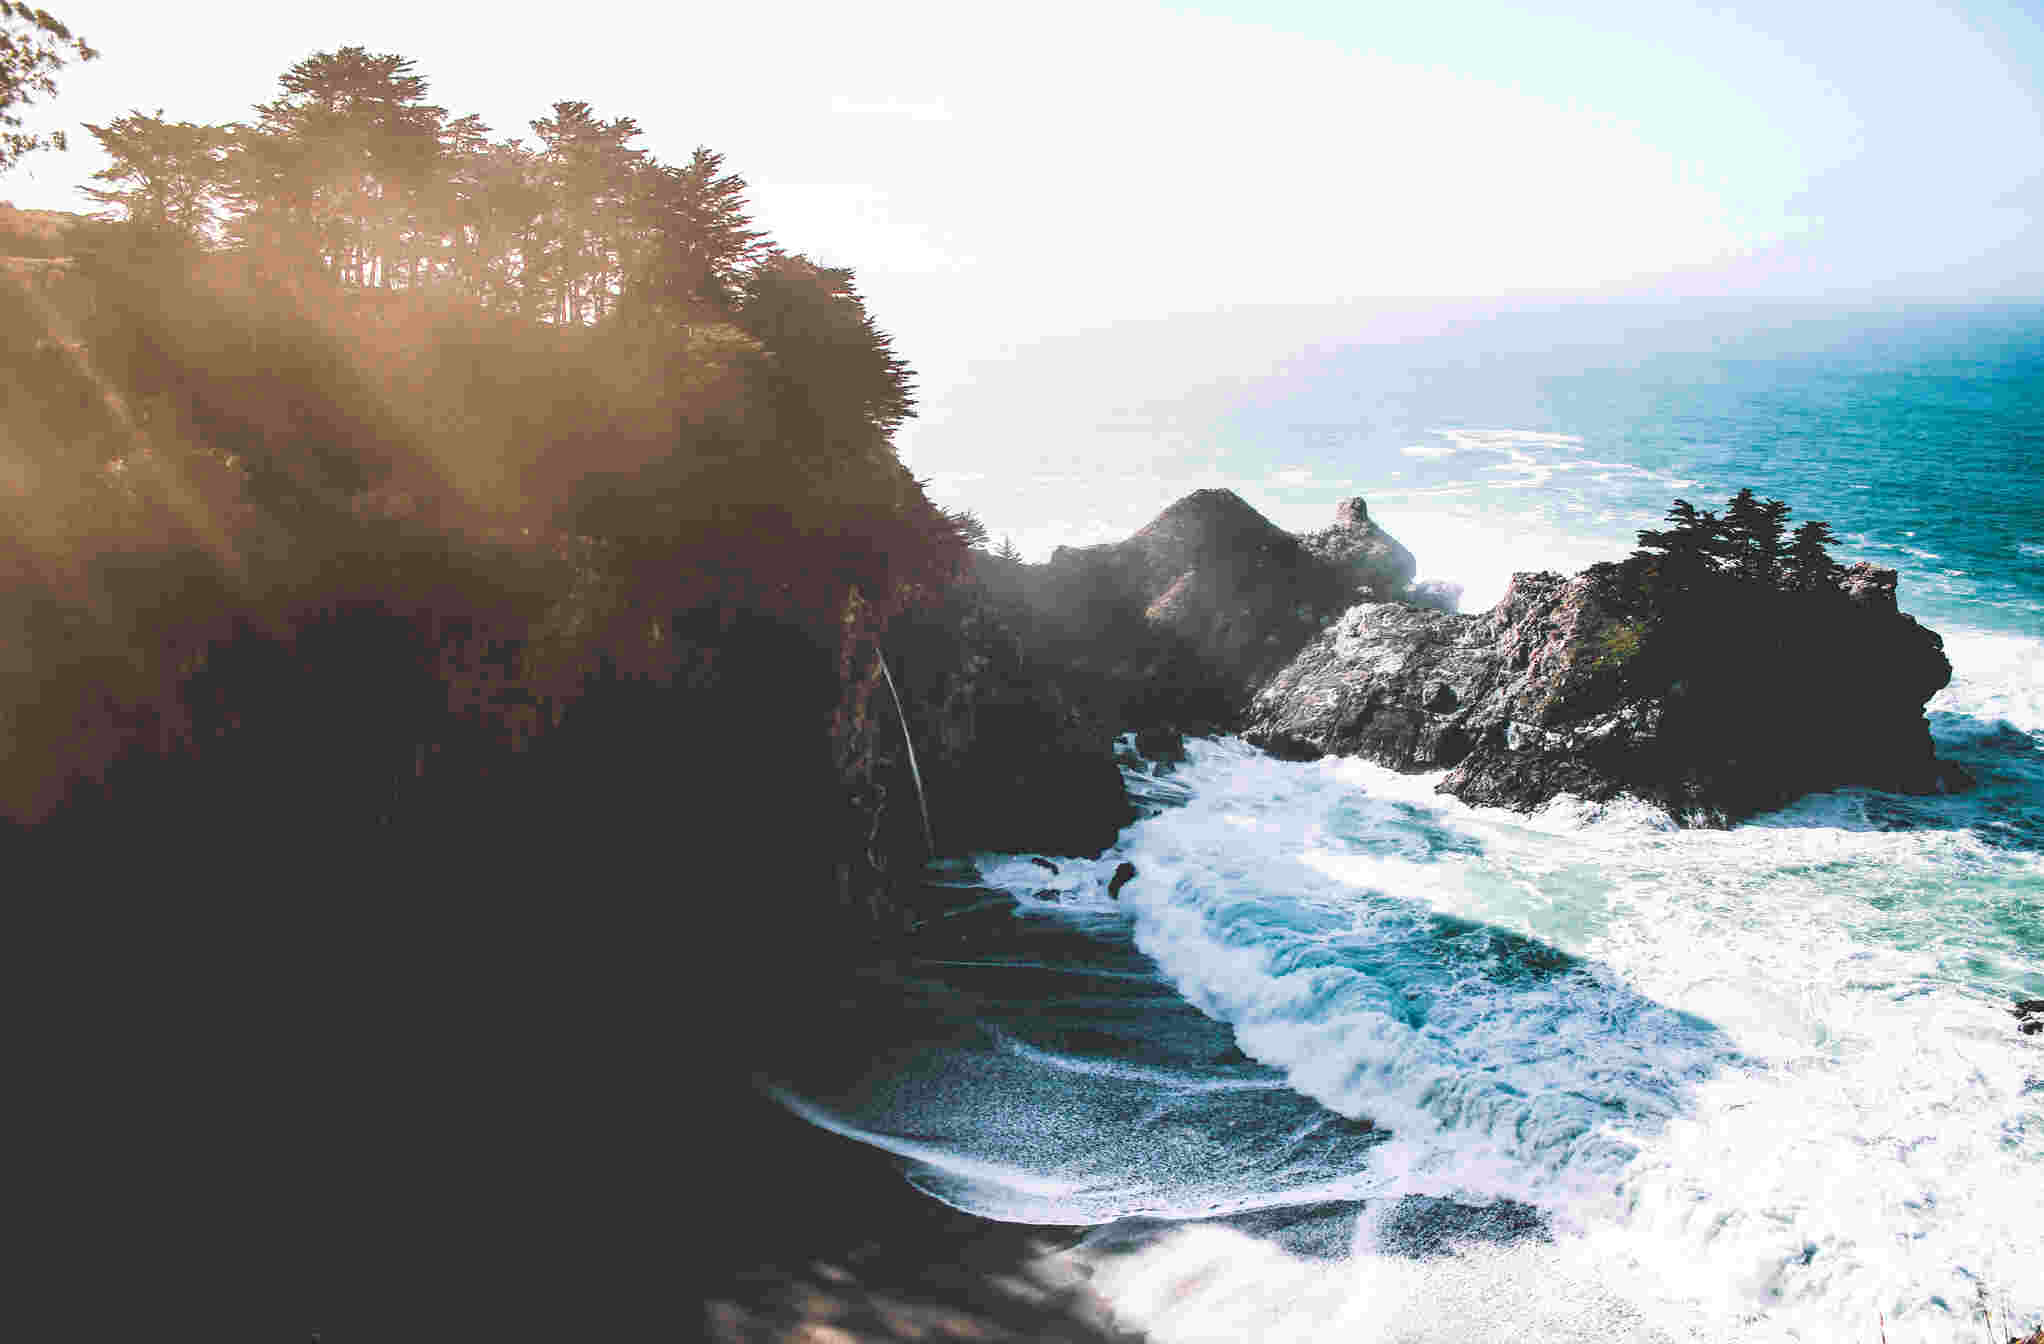
\includegraphics[width=\textwidth]{Images/jpeg/reconstructed/test1_10.png}
    \subcaption{$Q=10$}
    \end{subfigure}
    \begin{subfigure}[b]{0.49 \textwidth}
    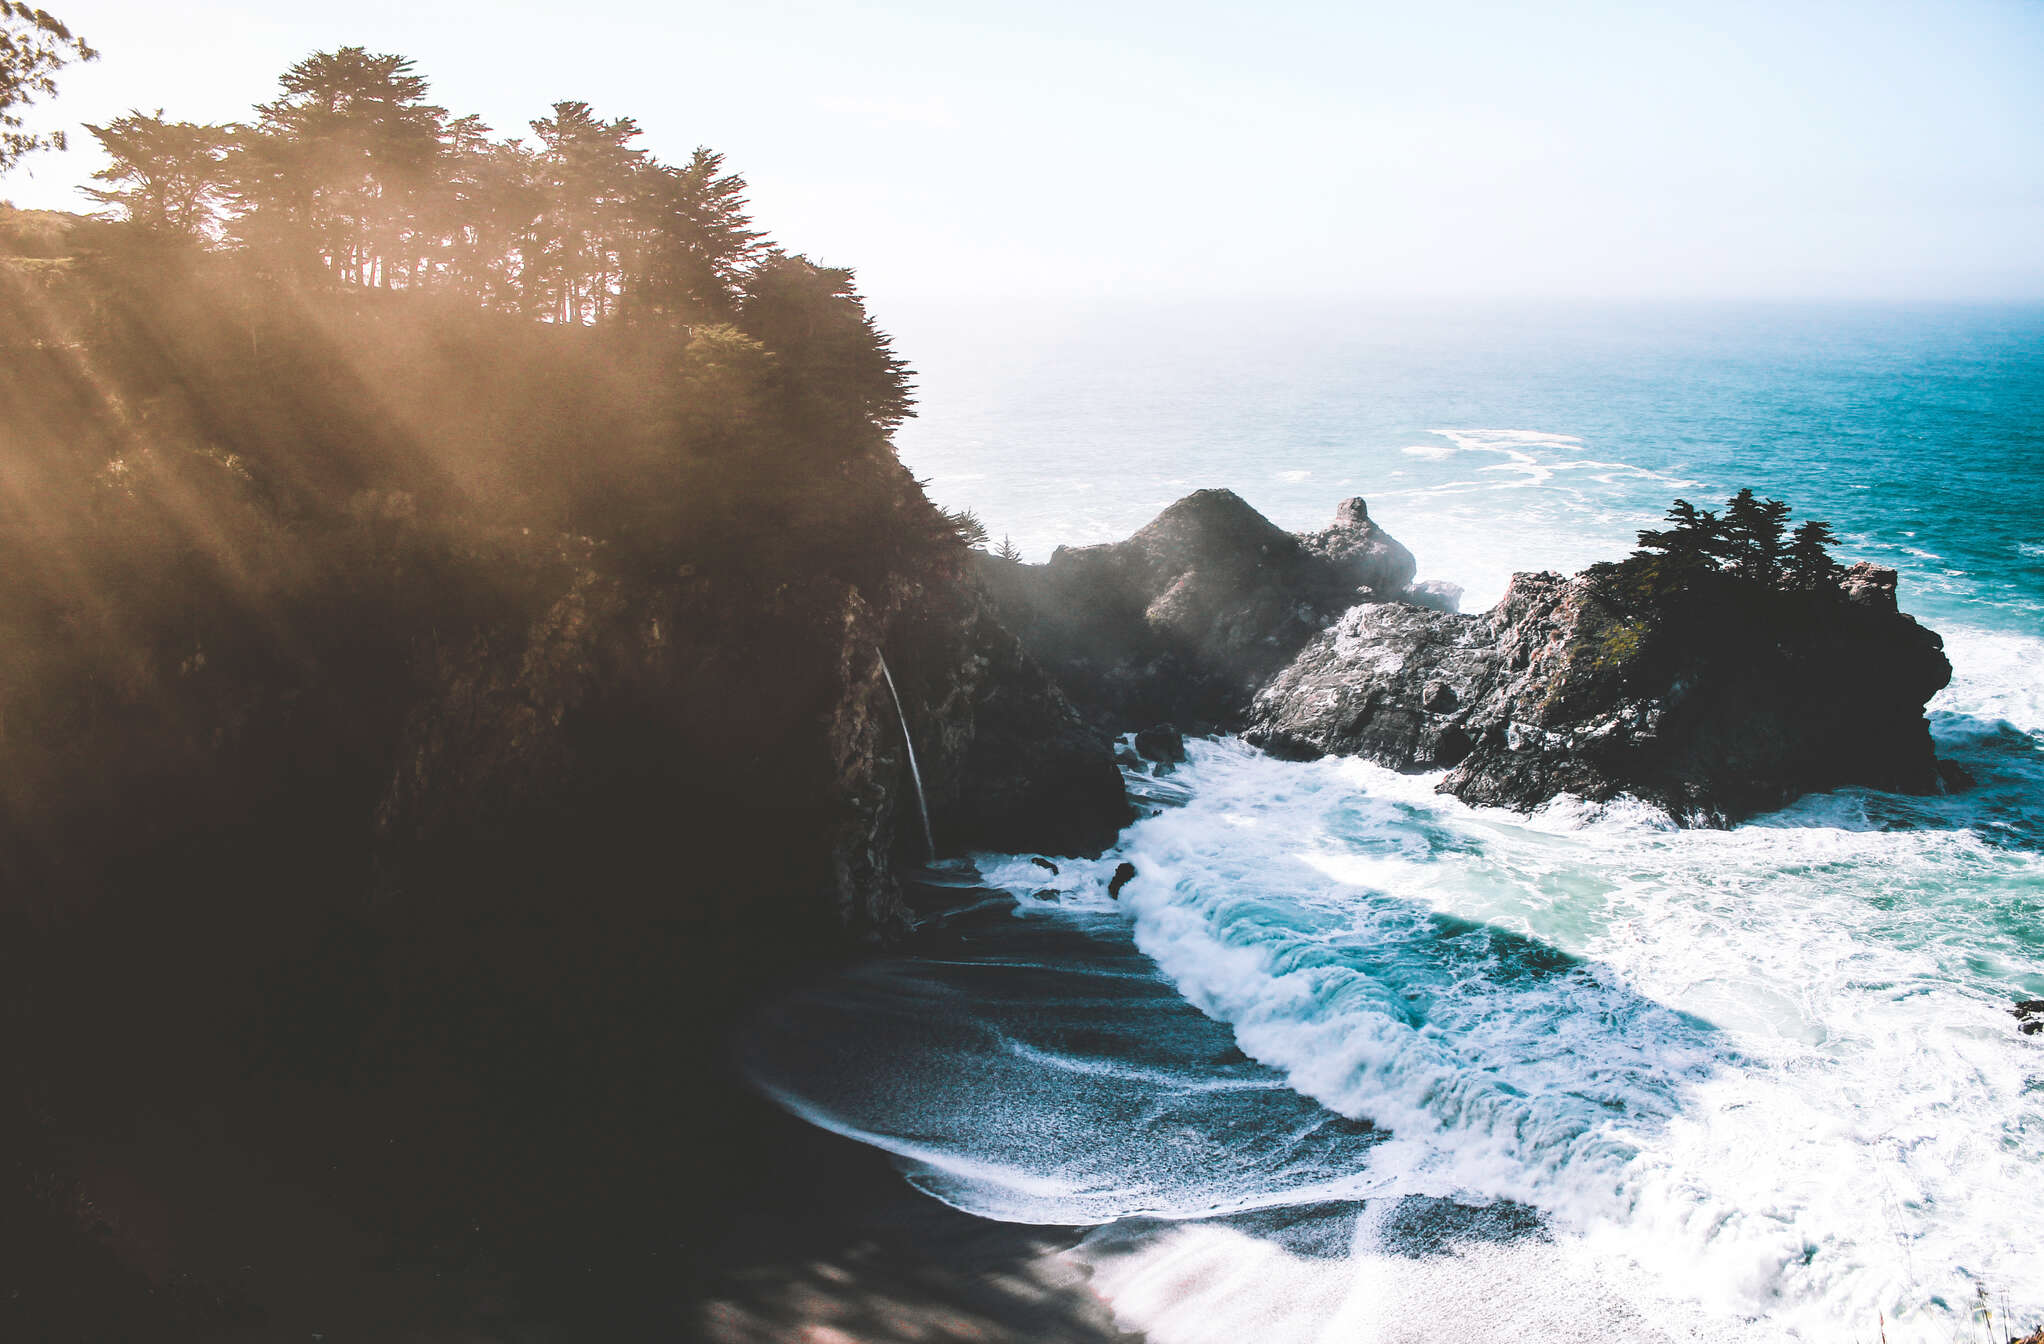
\includegraphics[width=\textwidth]{Images/jpeg/reconstructed/test1_60.png}
    \subcaption{$Q=60$}
    \end{subfigure}
    \begin{subfigure}[b]{0.49 \textwidth}
    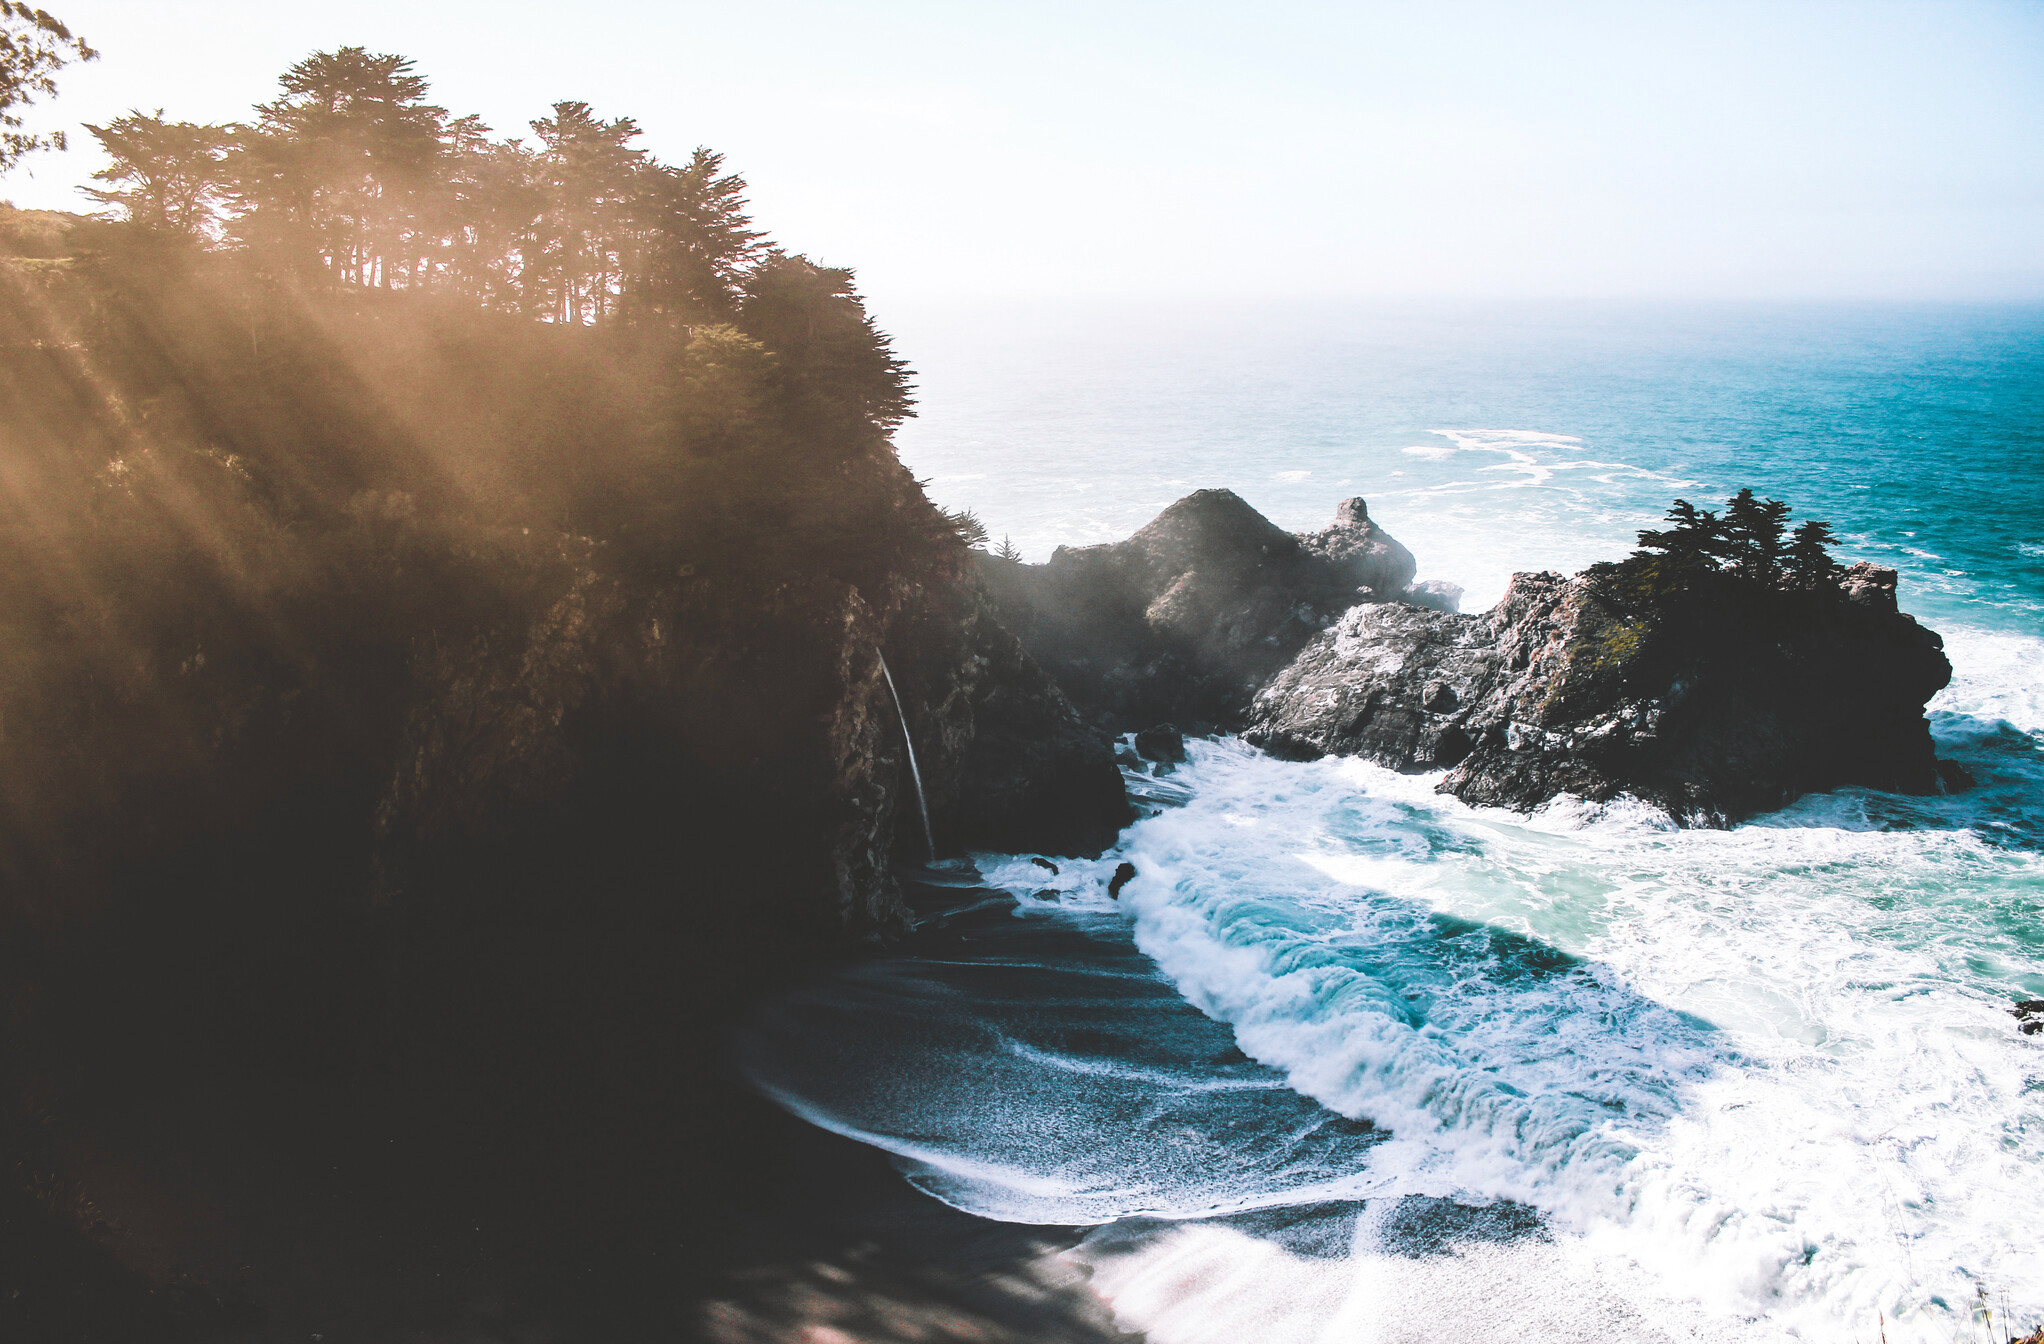
\includegraphics[width=\textwidth]{Images/jpeg/reconstructed/test1_90.png}
    \subcaption{$Q=90$}
    \end{subfigure}
    \begin{subfigure}[b]{0.49 \textwidth}
    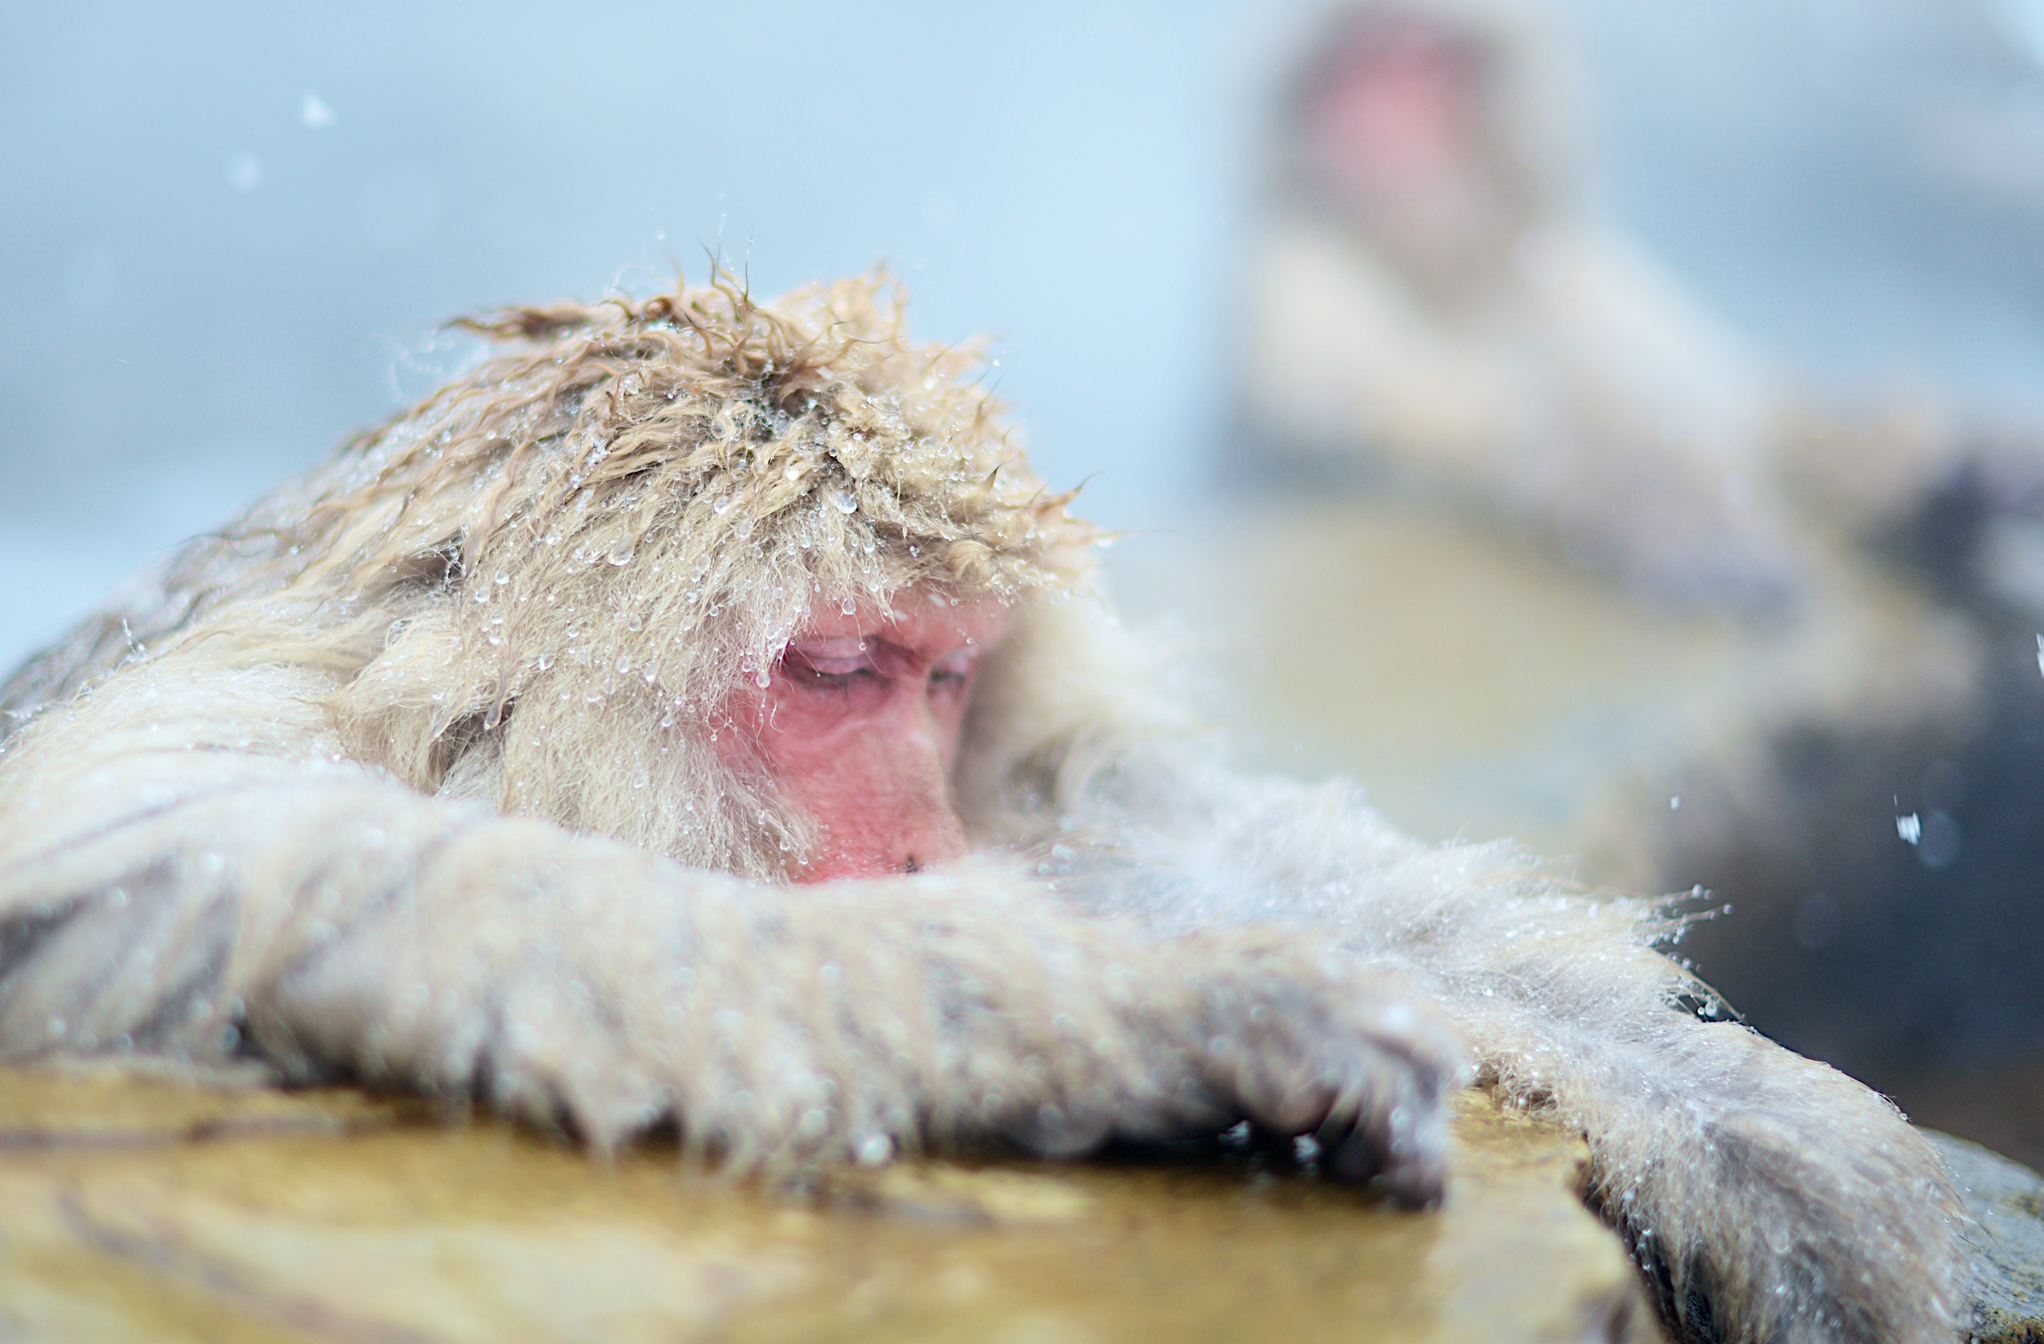
\includegraphics[width=\textwidth]{Images/test2.png}
    \subcaption{Original}
    \end{subfigure}
    \begin{subfigure}[b]{0.49 \textwidth}
    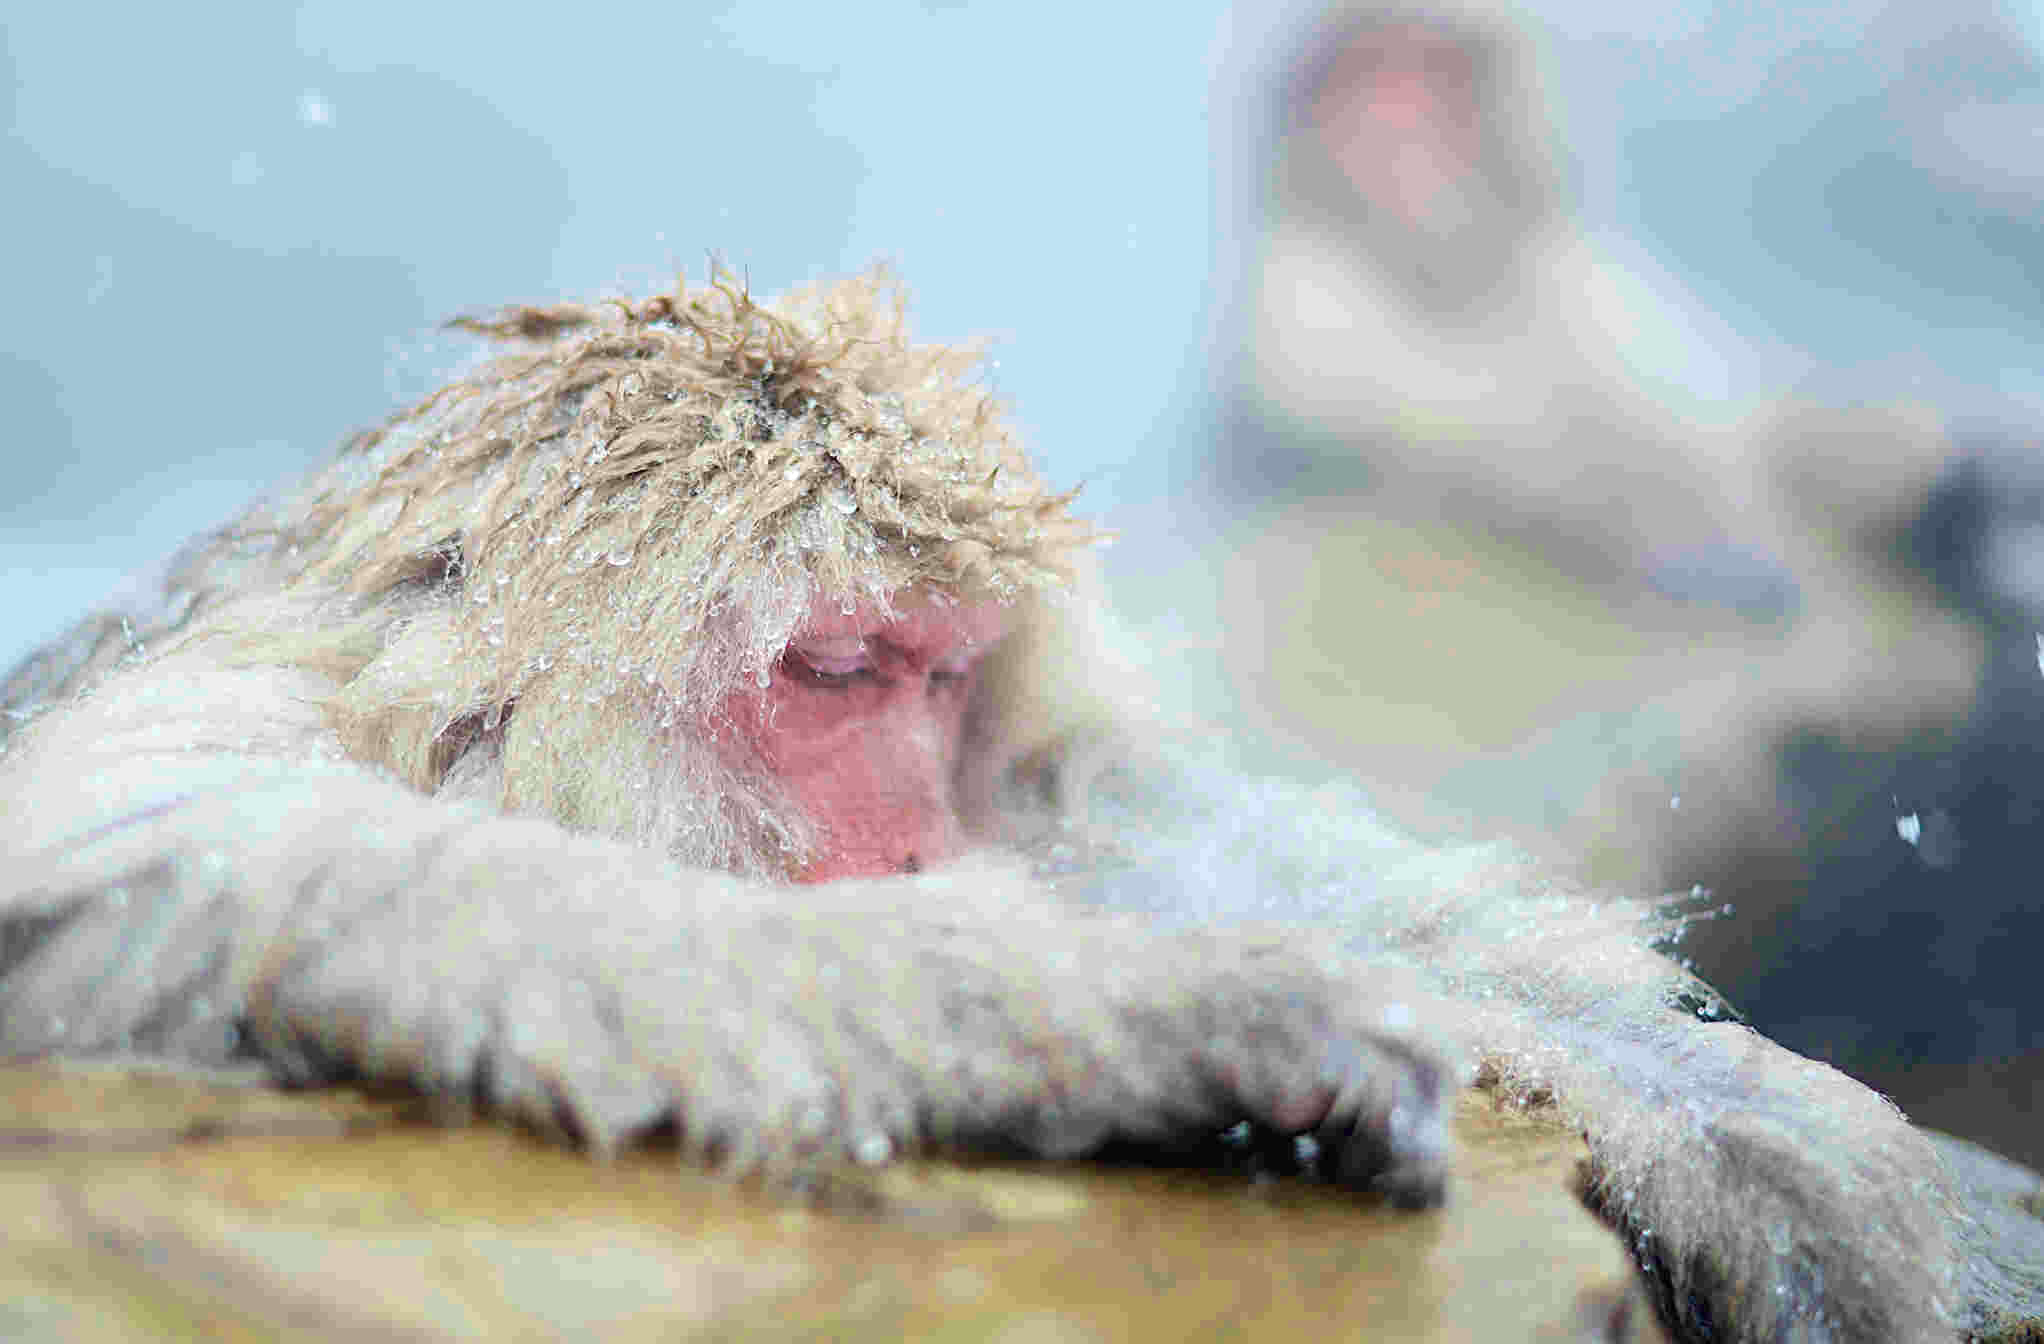
\includegraphics[width=\textwidth]{Images/jpeg/reconstructed/test2_10.png}
    \subcaption{$Q=10$}
    \end{subfigure}
    \begin{subfigure}[b]{0.49 \textwidth}
    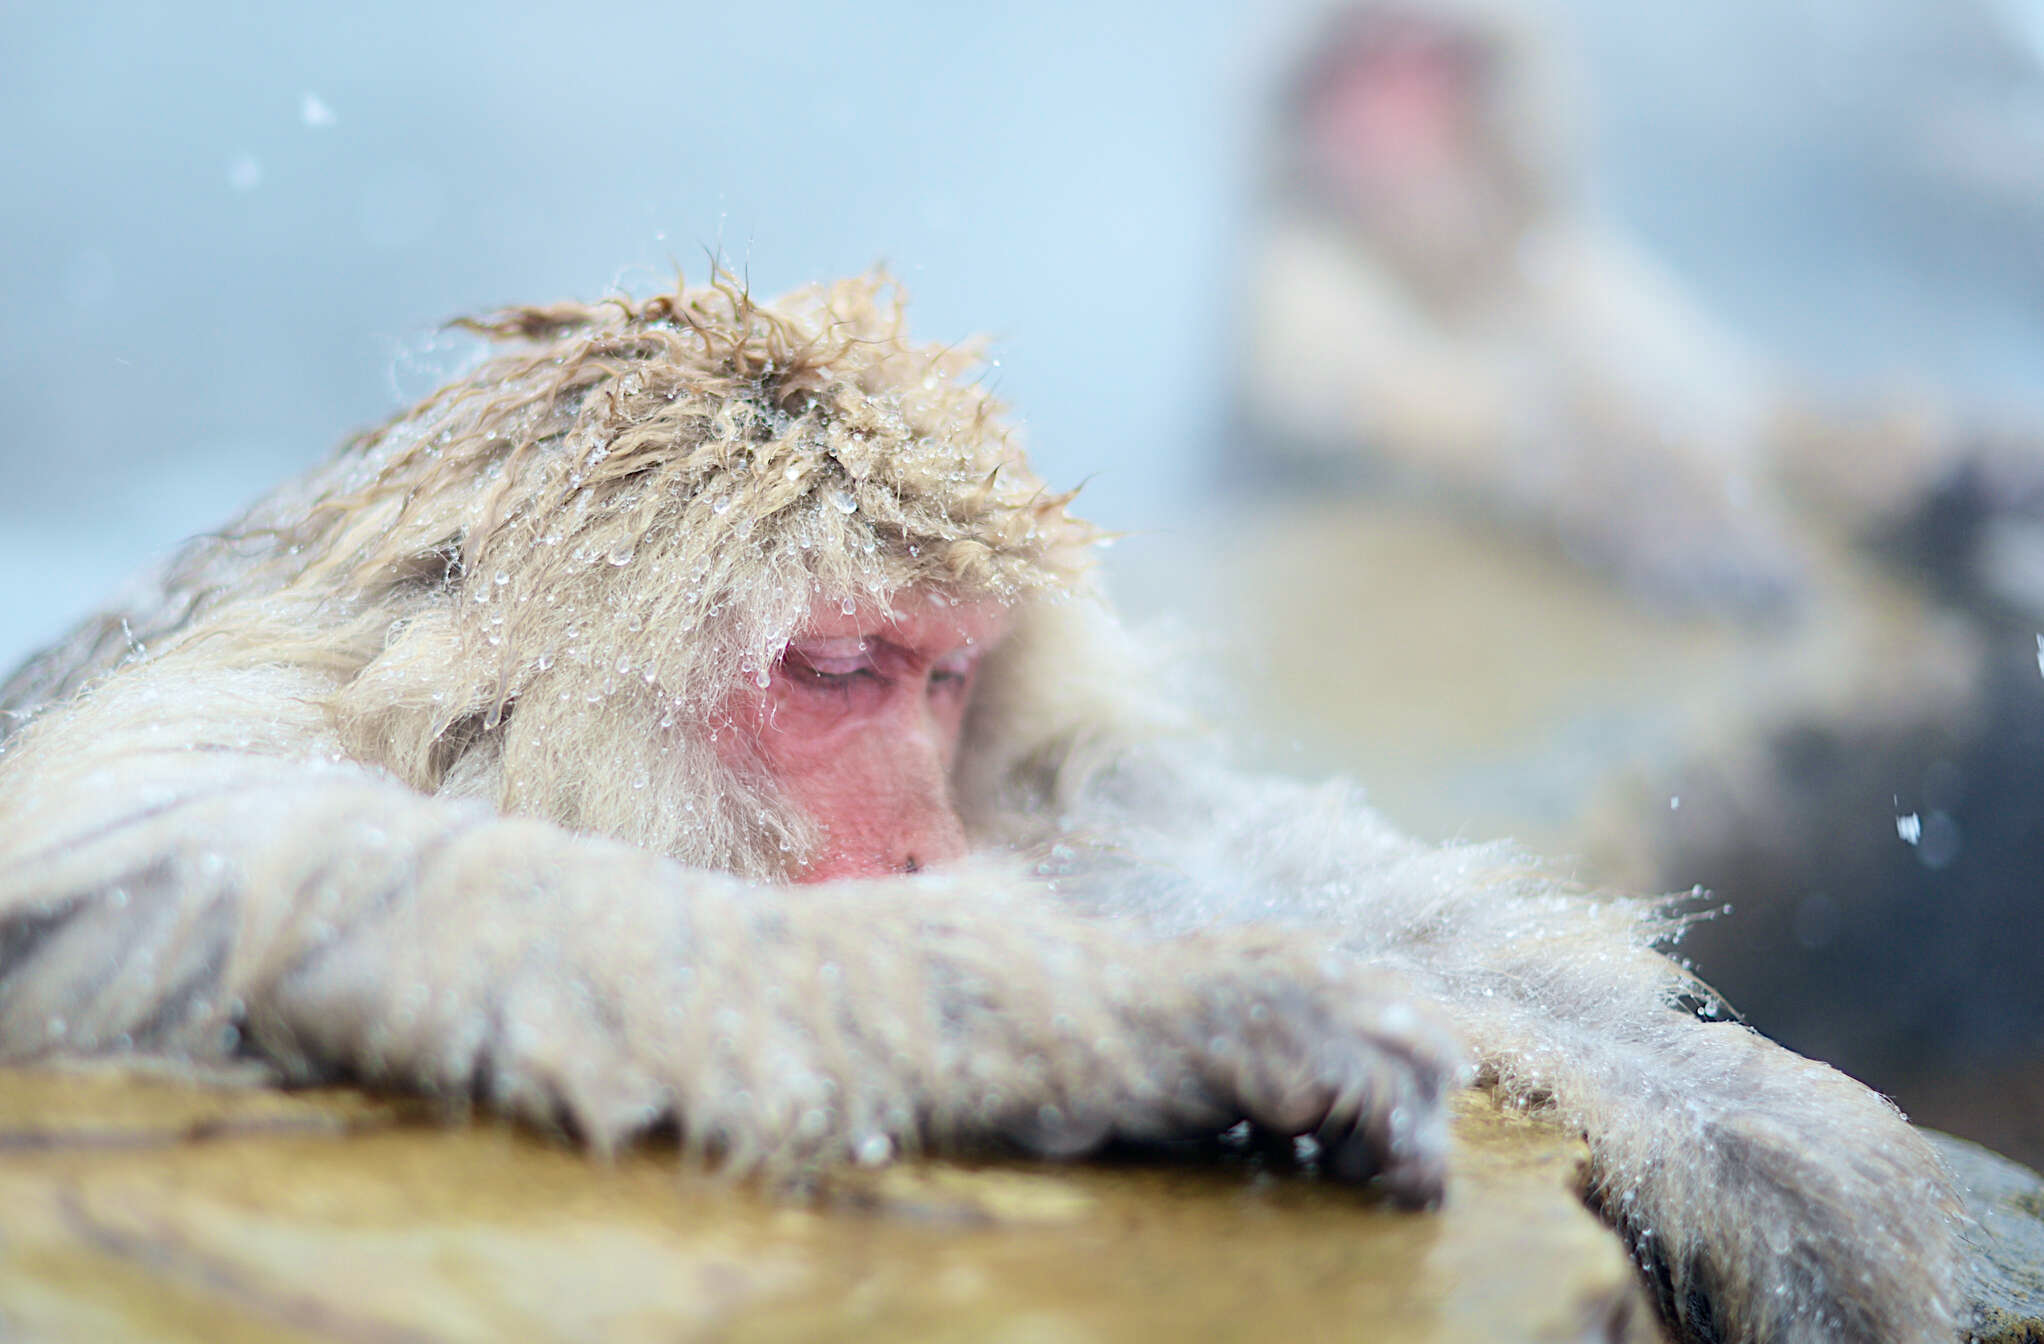
\includegraphics[width=\textwidth]{Images/jpeg/reconstructed/test2_60.png}
    \subcaption{$Q=60$}
    \end{subfigure}
    \begin{subfigure}[b]{0.49 \textwidth}
    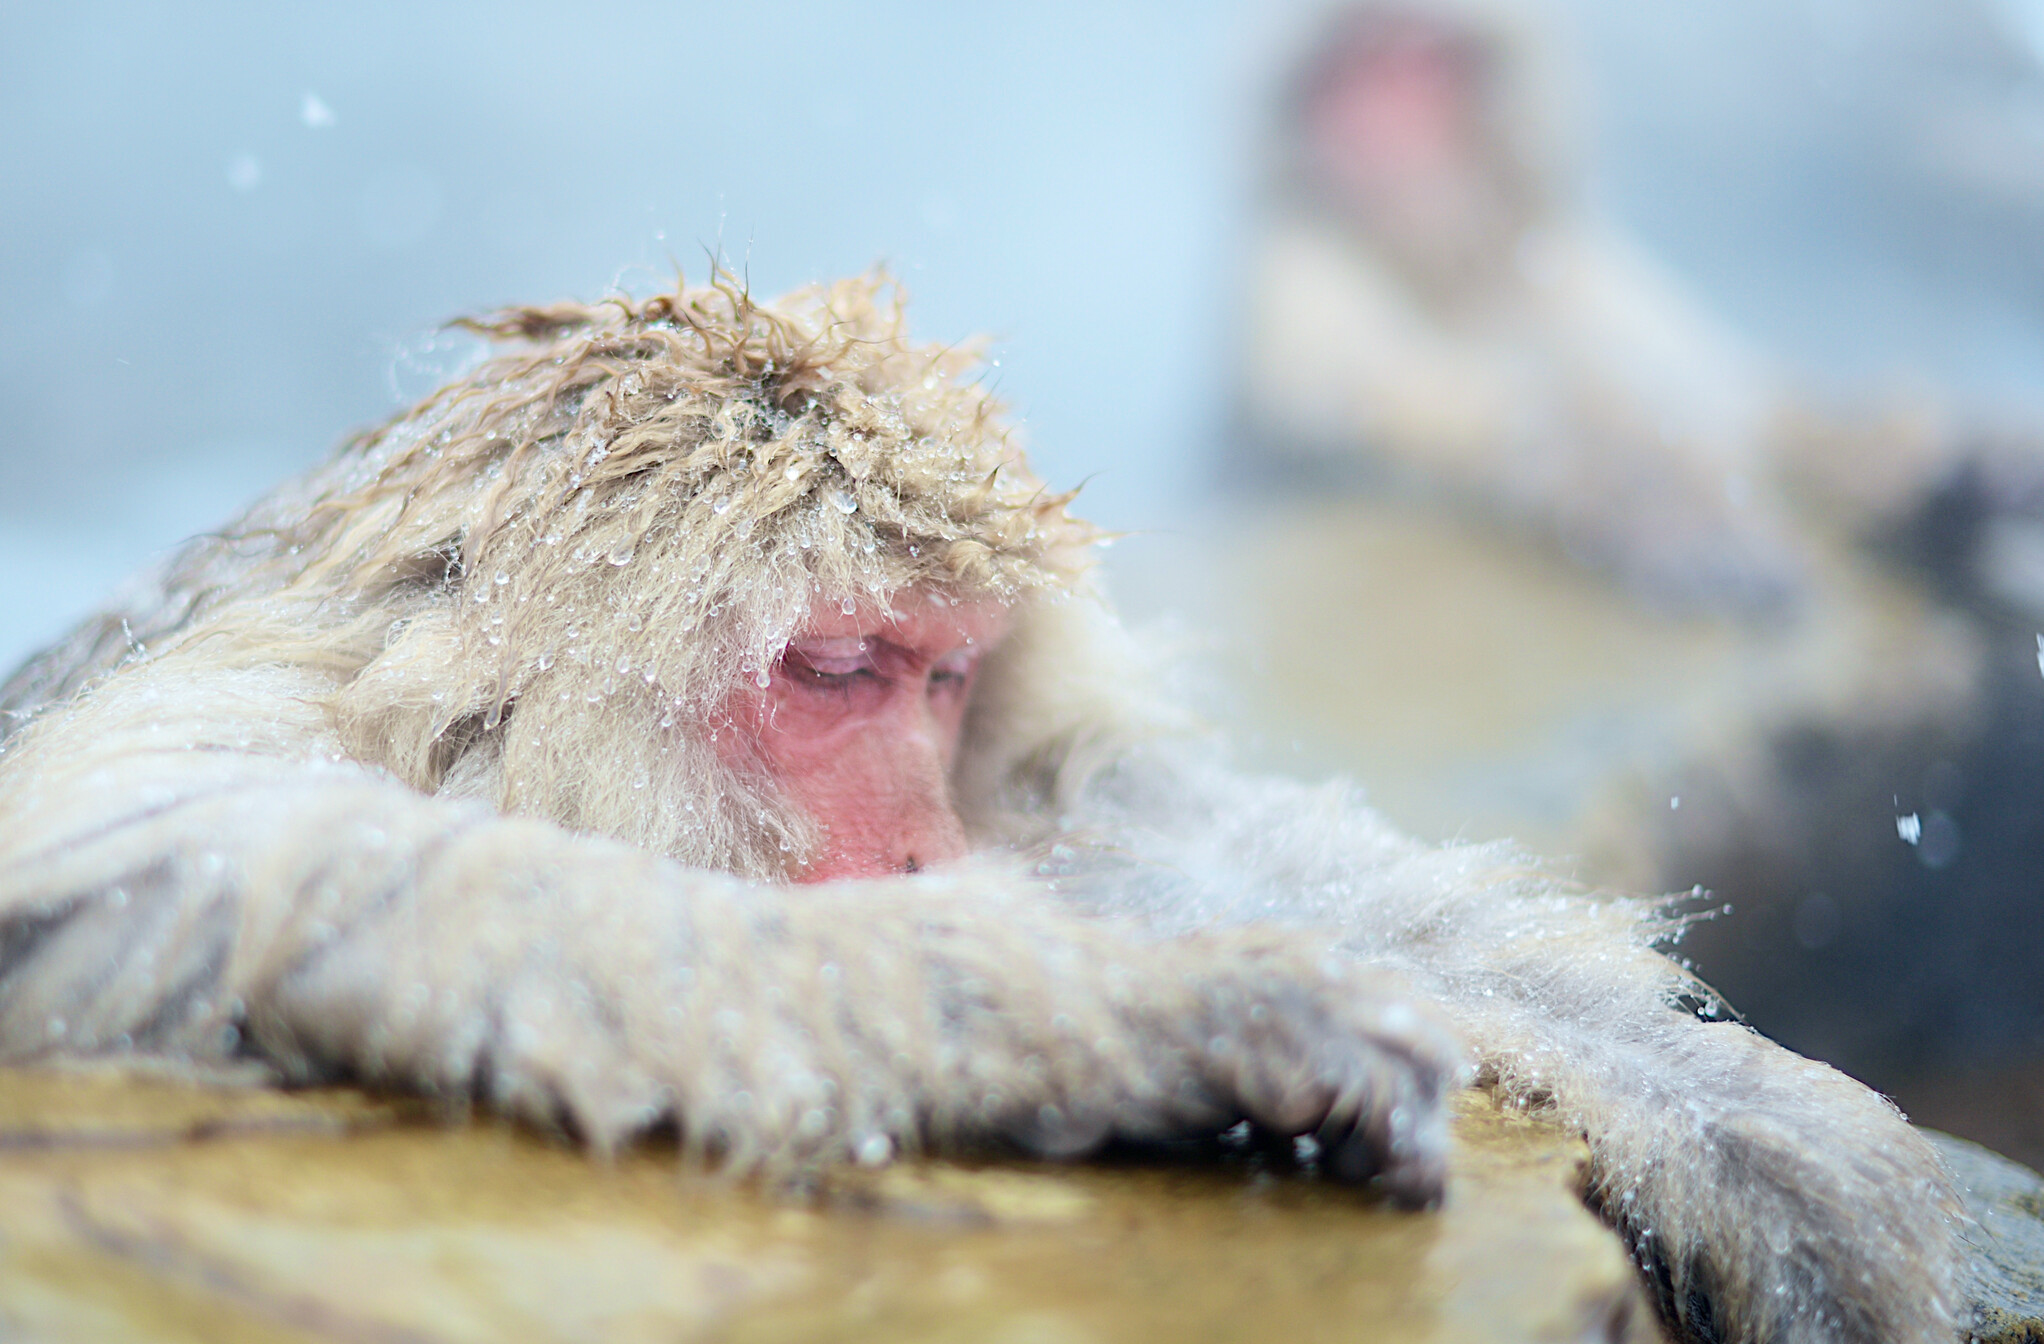
\includegraphics[width=\textwidth]{Images/jpeg/reconstructed/test2_90.png}
    \subcaption{$Q=90$}
    \end{subfigure}
    \end{figure}

\begin{figure}
 \ContinuedFloat
    \begin{subfigure}[b]{0.49 \textwidth}
    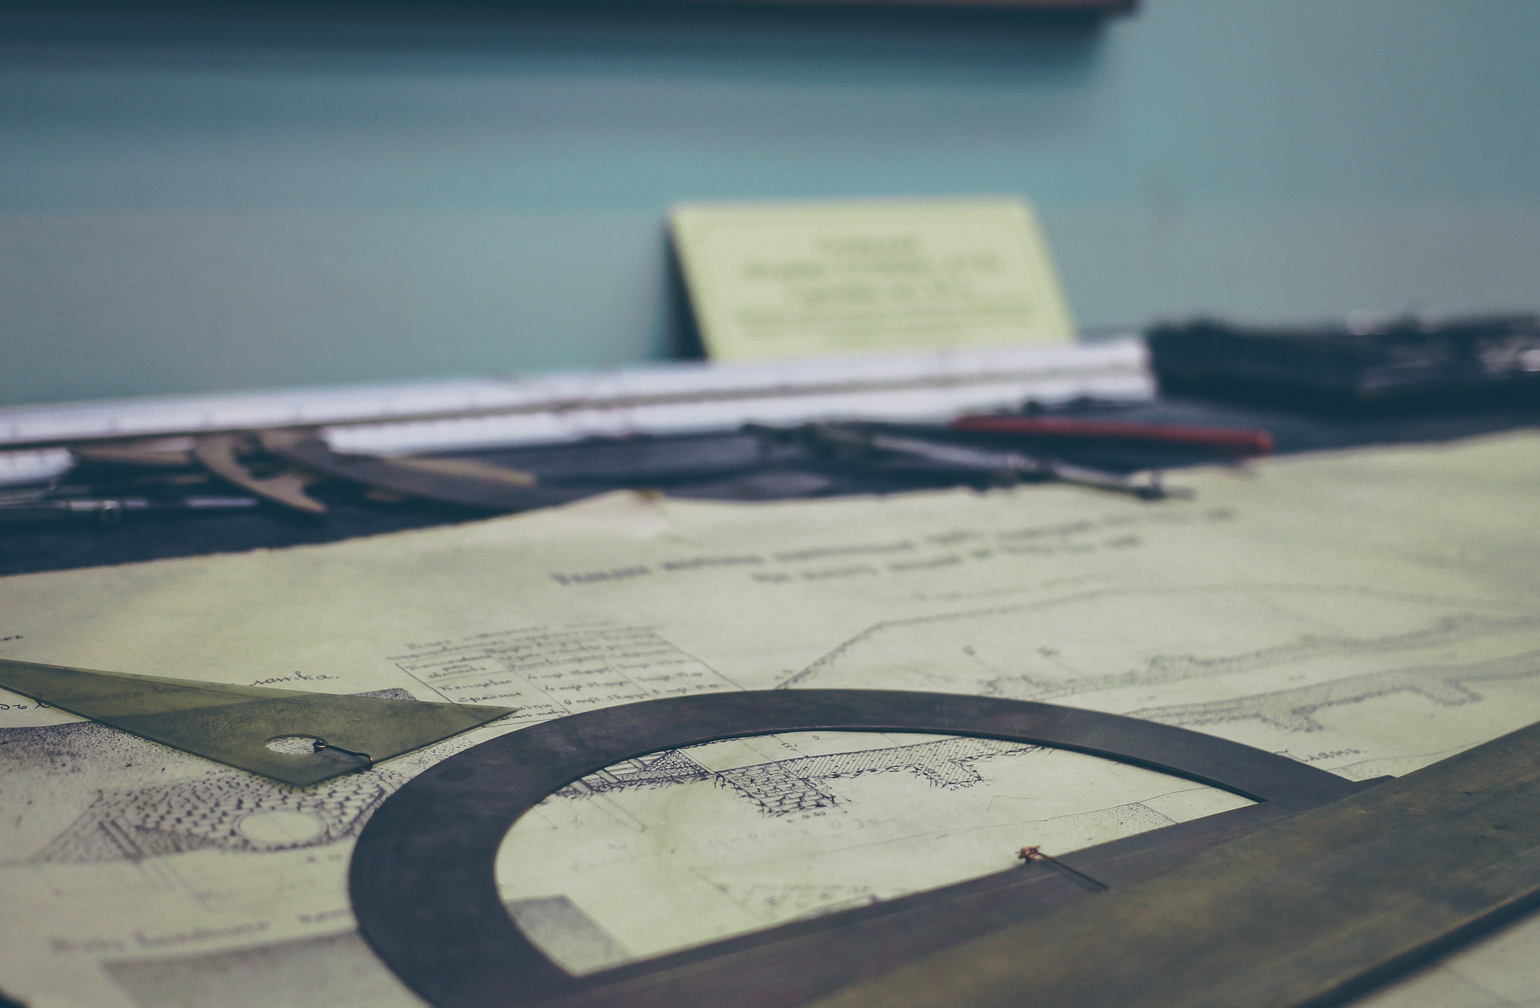
\includegraphics[width=\textwidth]{Images/test3.png}
    \subcaption{Original}
    \end{subfigure}
    \begin{subfigure}[b]{0.49 \textwidth}
    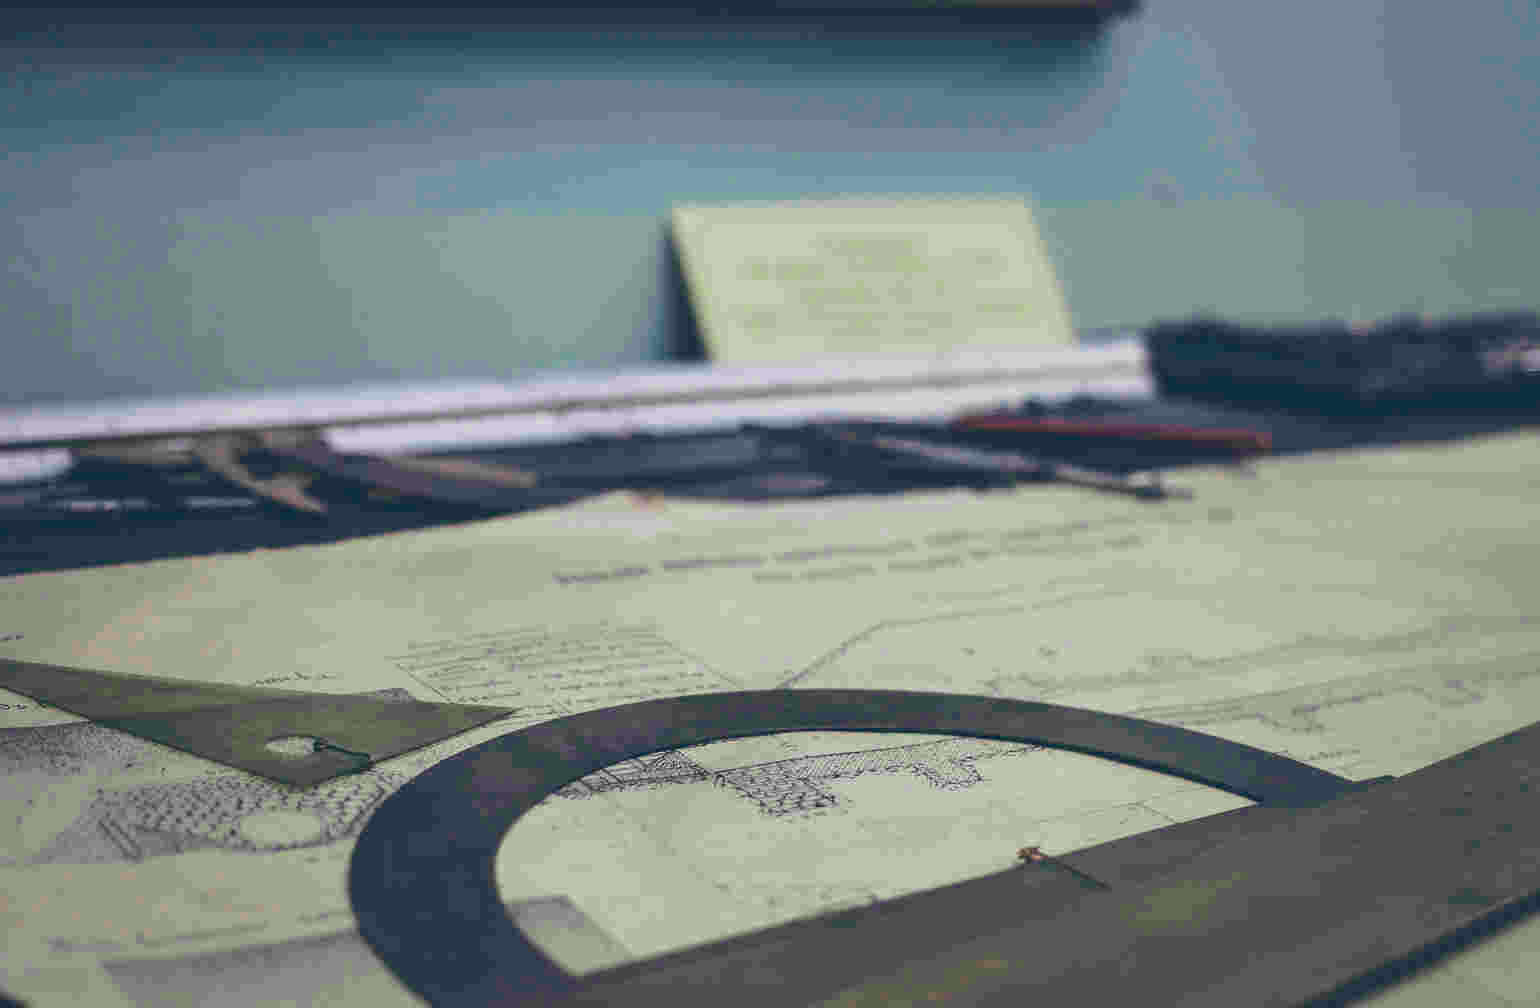
\includegraphics[width=\textwidth]{Images/jpeg/reconstructed/test3_10.png}
    \subcaption{$Q=10$}
    \end{subfigure}
    \begin{subfigure}[b]{0.49 \textwidth}
    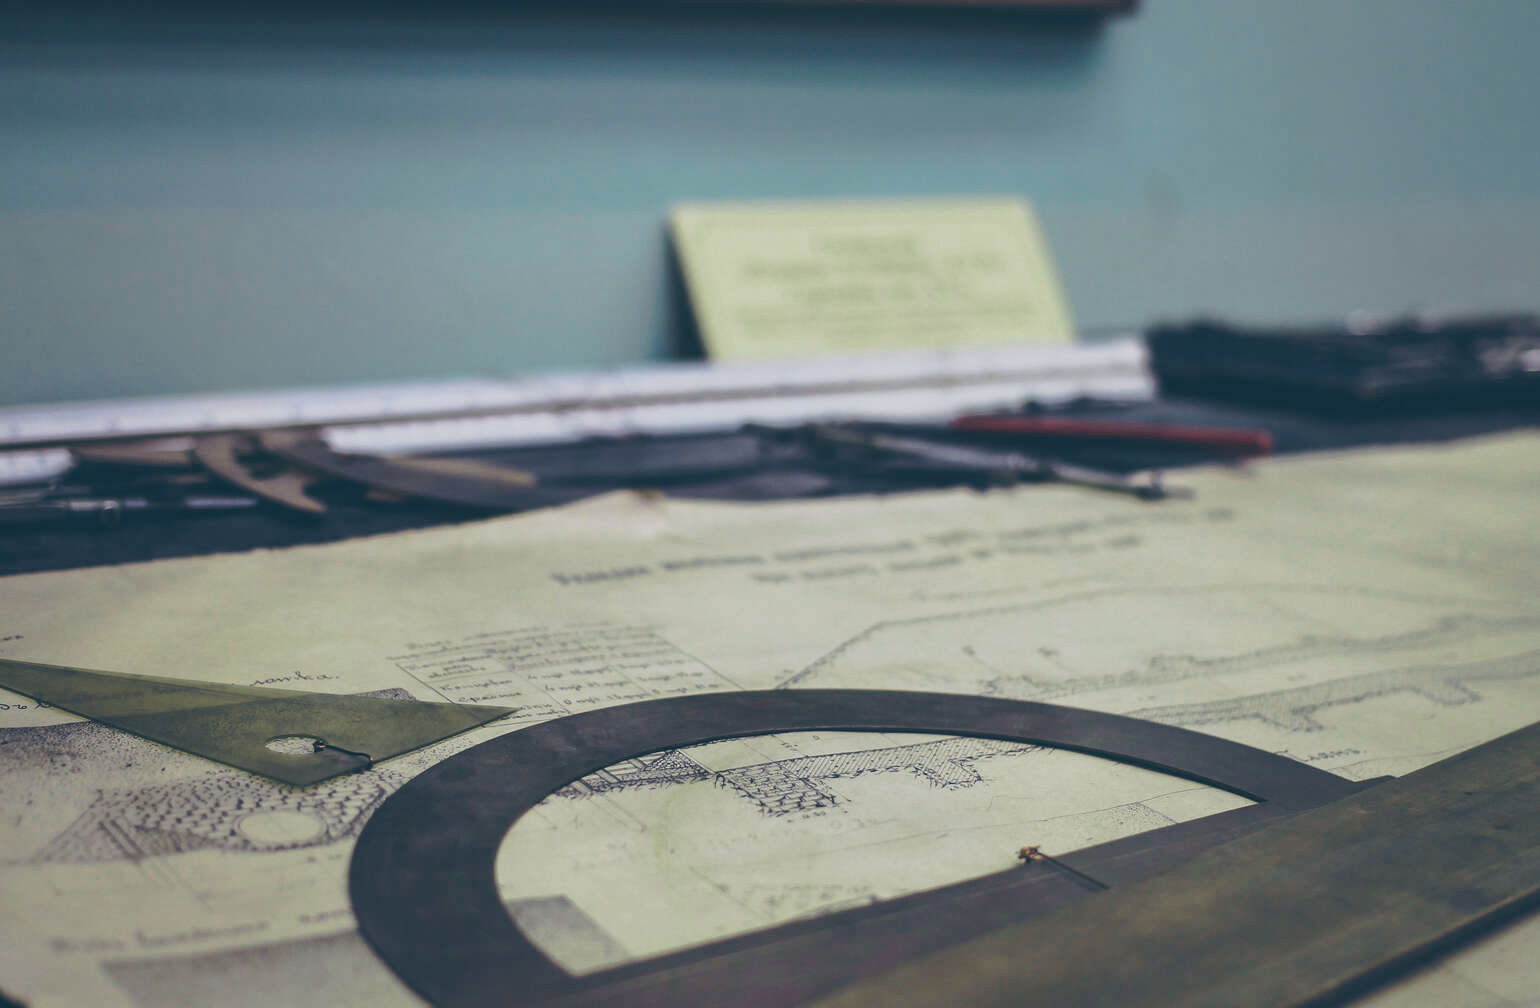
\includegraphics[width=\textwidth]{Images/jpeg/reconstructed/test3_60.png}
    \subcaption{$Q=60$}
    \end{subfigure}
    \begin{subfigure}[b]{0.49 \textwidth}
    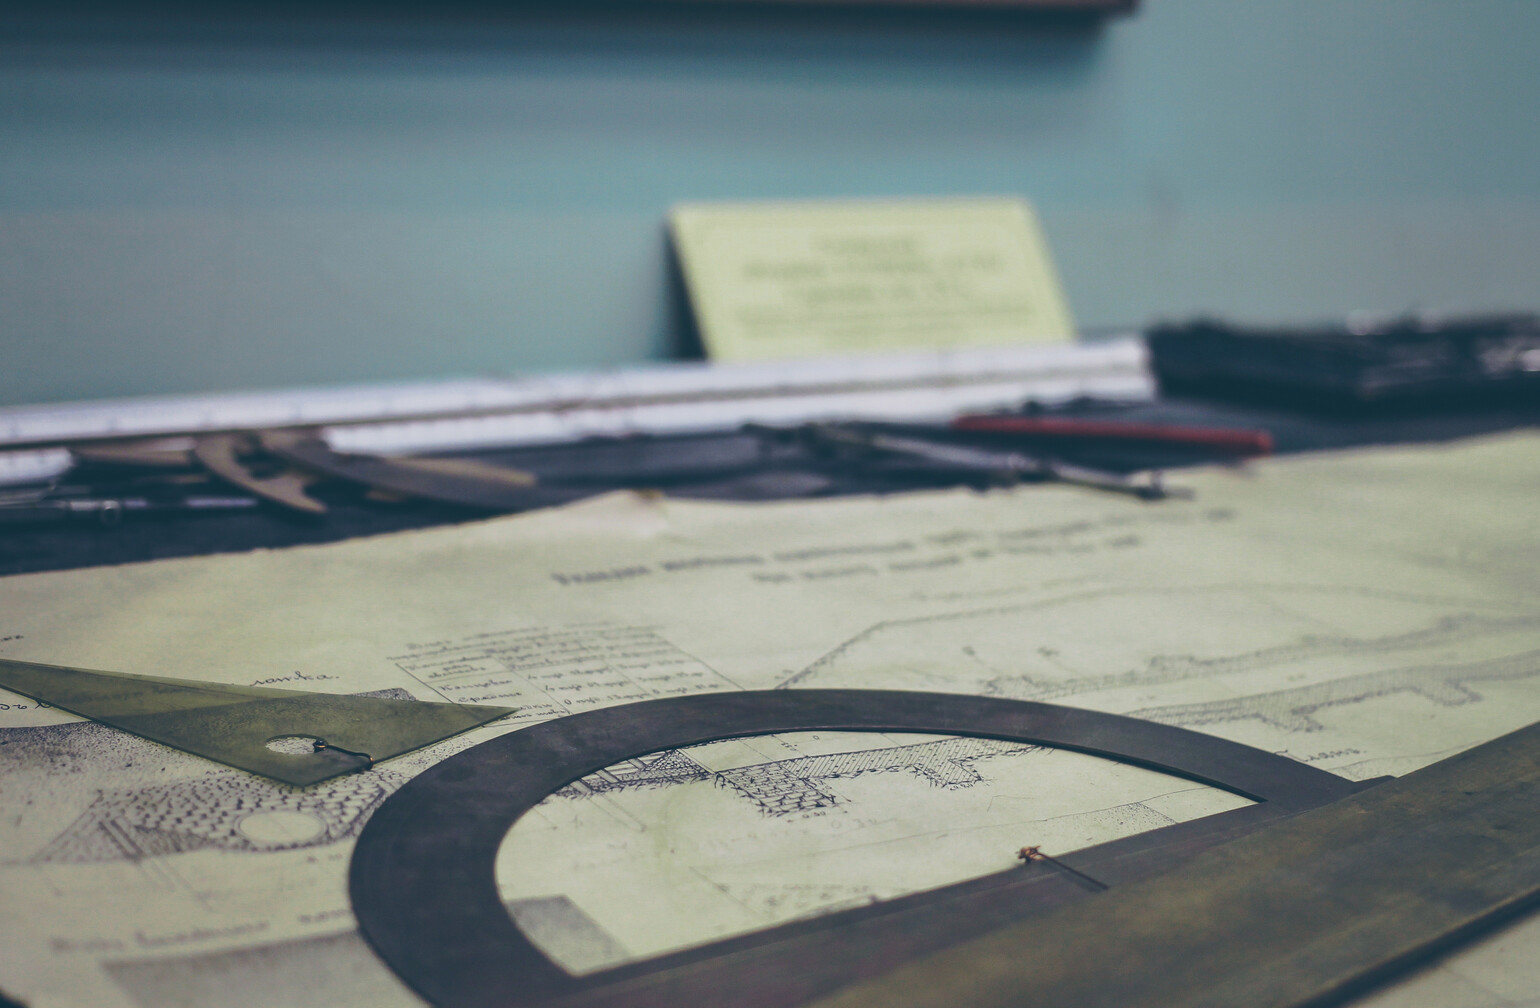
\includegraphics[width=\textwidth]{Images/jpeg/reconstructed/test3_90.png}
    \subcaption{$Q=90$}
    \end{subfigure}
    \caption{JPEG compression for different Q values on different test images.}
    \label{fig:jpeg}
\end{figure}

\begin{table}[]
    \centering
    \caption{bpp values for JPEG compression using different Q-values.}
    \begin{tabular}{c|c c}
        input & Q-value & bpp \\
        \hline 
        \hline
        \textsf{test1}& 10 & 0.32 \\
        & 60 & 0.8\\
        & 90 & 1.95 \\
        \hline
        \textsf{test2}& 10 & 0.27 \\
        & 60 & 0.58\\
        & 90 & 1.61\\
        \hline
        \textsf{test3}& 10 & 0.15 \\
        & 60 & 0.27 \\
        & 90 & 0.79\\
    \end{tabular}
    \label{tab:jpeg_bpp}
\end{table}

%---------------------------
% Task 2
%---------------------------
\section{Auto-encoder for Image Compression}
In this exercise, we were asked to design an auto-encoder architecture and perform hyperparameter fine-tuning such that the auto-encoder generates images which are visually as close as possible to the reference image. In the following, the steps for improving the visual performance of the auto-encoder are listed.\\

First, all initial configurations (number of layers, layer dimensions, number of epochs, activation function, learning rate, etc.) were kept unchanged and only the size of the latent space was varied. The size was chosen to be multiples of 10. The best reconstructed images were achieved for a latent space of size $80$. The respective results can seen in Figure \ref{fig:auto_latent}. Increasing the latent space further lead to the creation of patterns in the reconstructed version (cf. Figure \ref{fig:auto_latent} with latent space size $s=90$). Table \ref{tab:auto_bpp} reports the bpp values for this initial architecture.\\

\begin{table}[]
    \centering
    \caption{bpp values for auto-encoder compression using different latent sizes $s$.}
    \begin{tabular}{c|c c}
        input & size of latent space  & bpp \\
        \hline 
        \hline
        \textsf{test1, test2, test3} & 10 & 1.22 \\
         & 80 & 9.8\\
        & 90 & 11.02\\
    \end{tabular}
    \label{tab:auto_bpp}
\end{table}

\begin{figure}
    \centering
    \begin{subfigure}[b]{0.49 \textwidth}
    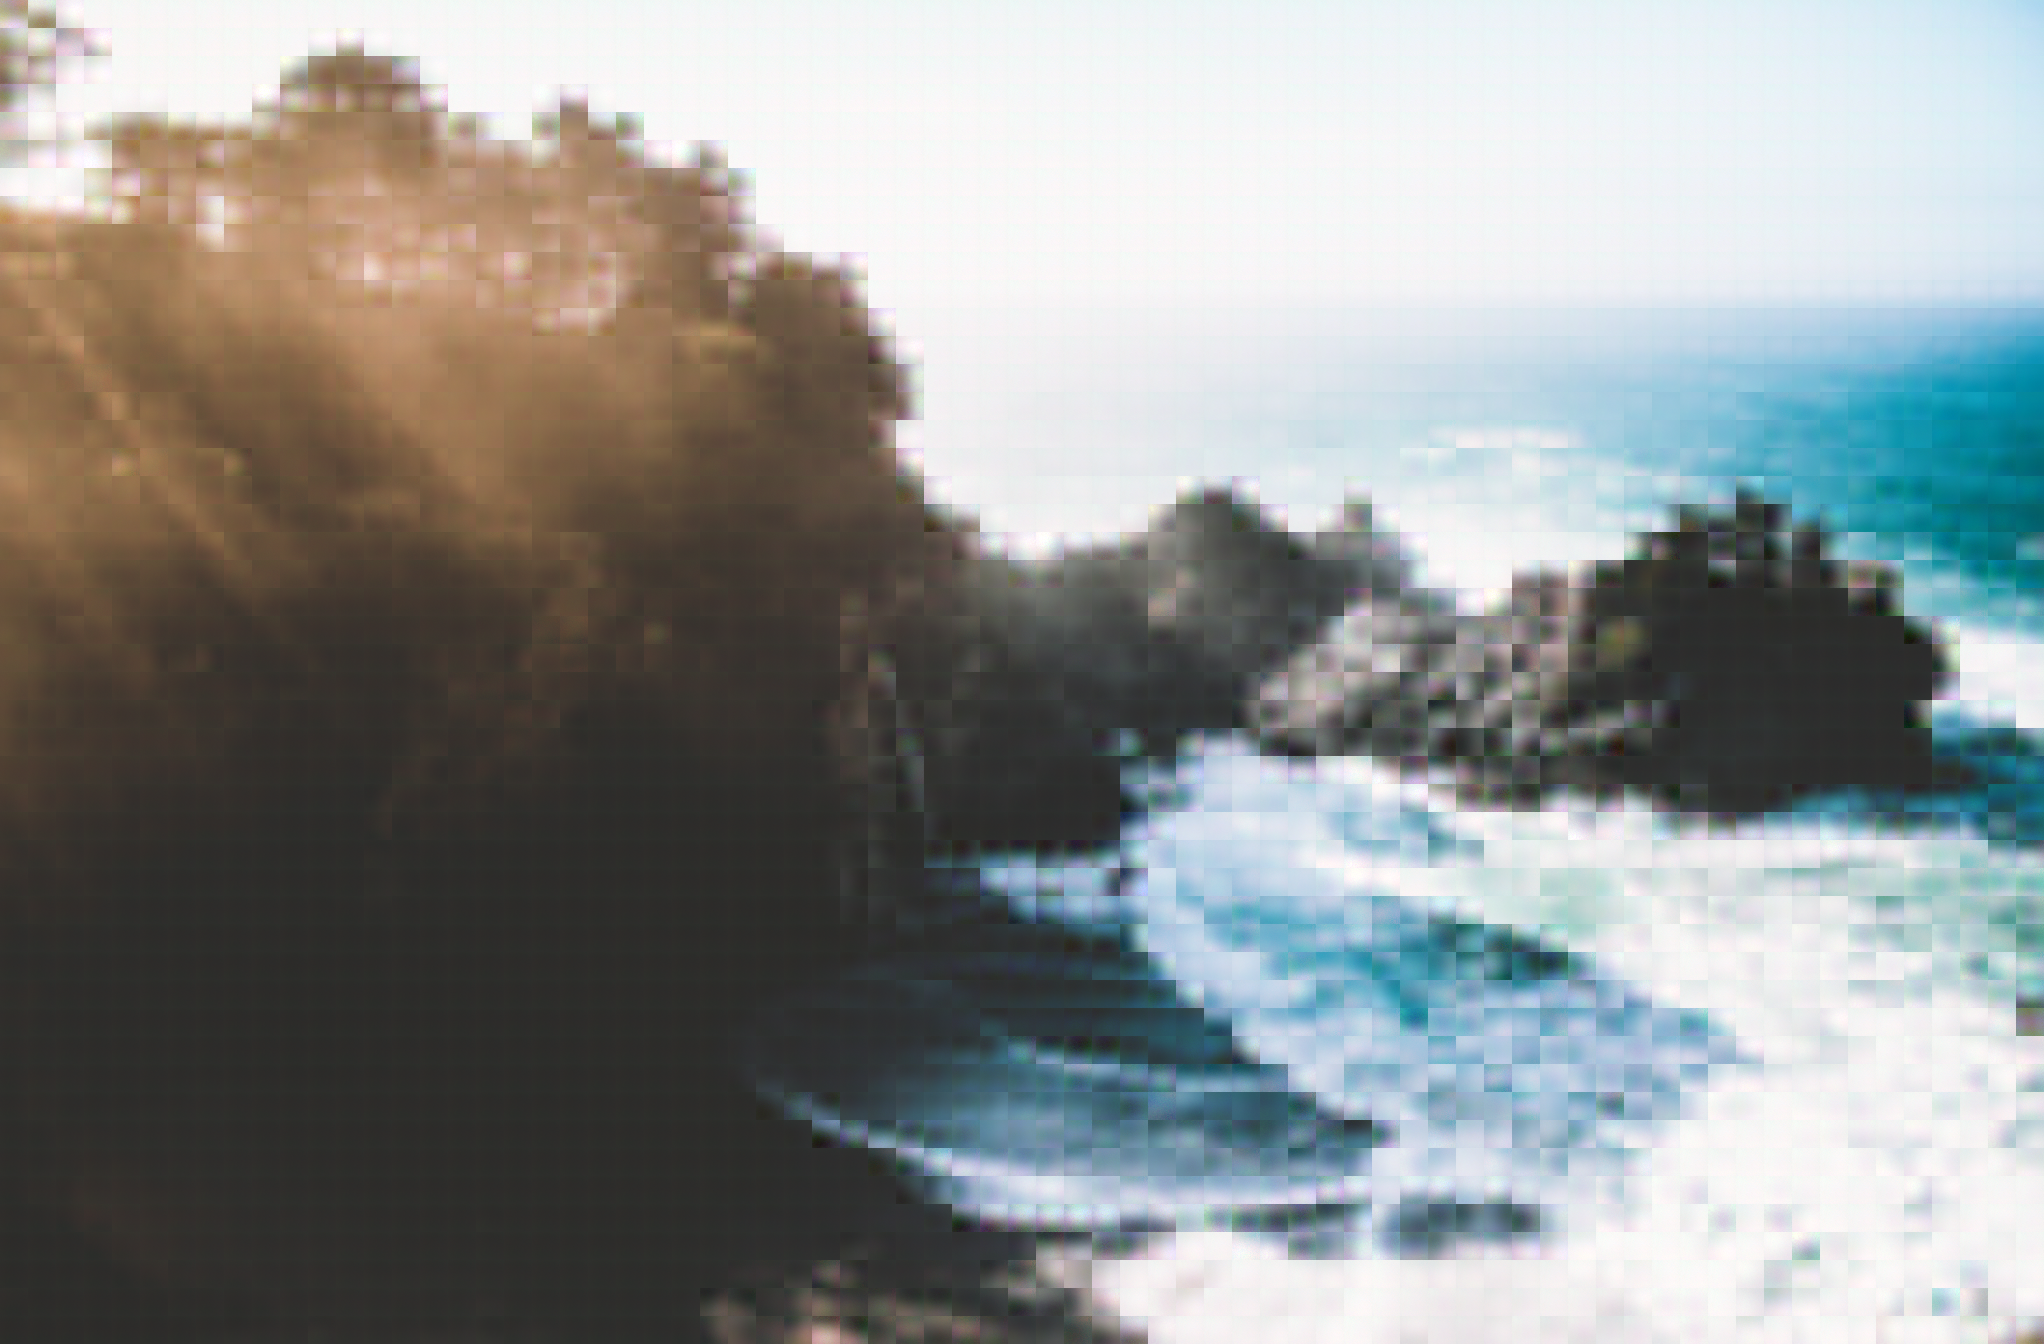
\includegraphics[width=\textwidth]{Images/autoencoder/reconstructed/500/test1_10.png}
    \subcaption{$s=10$}
    \end{subfigure}
    \centering
    \begin{subfigure}[b]{0.49 \textwidth}
    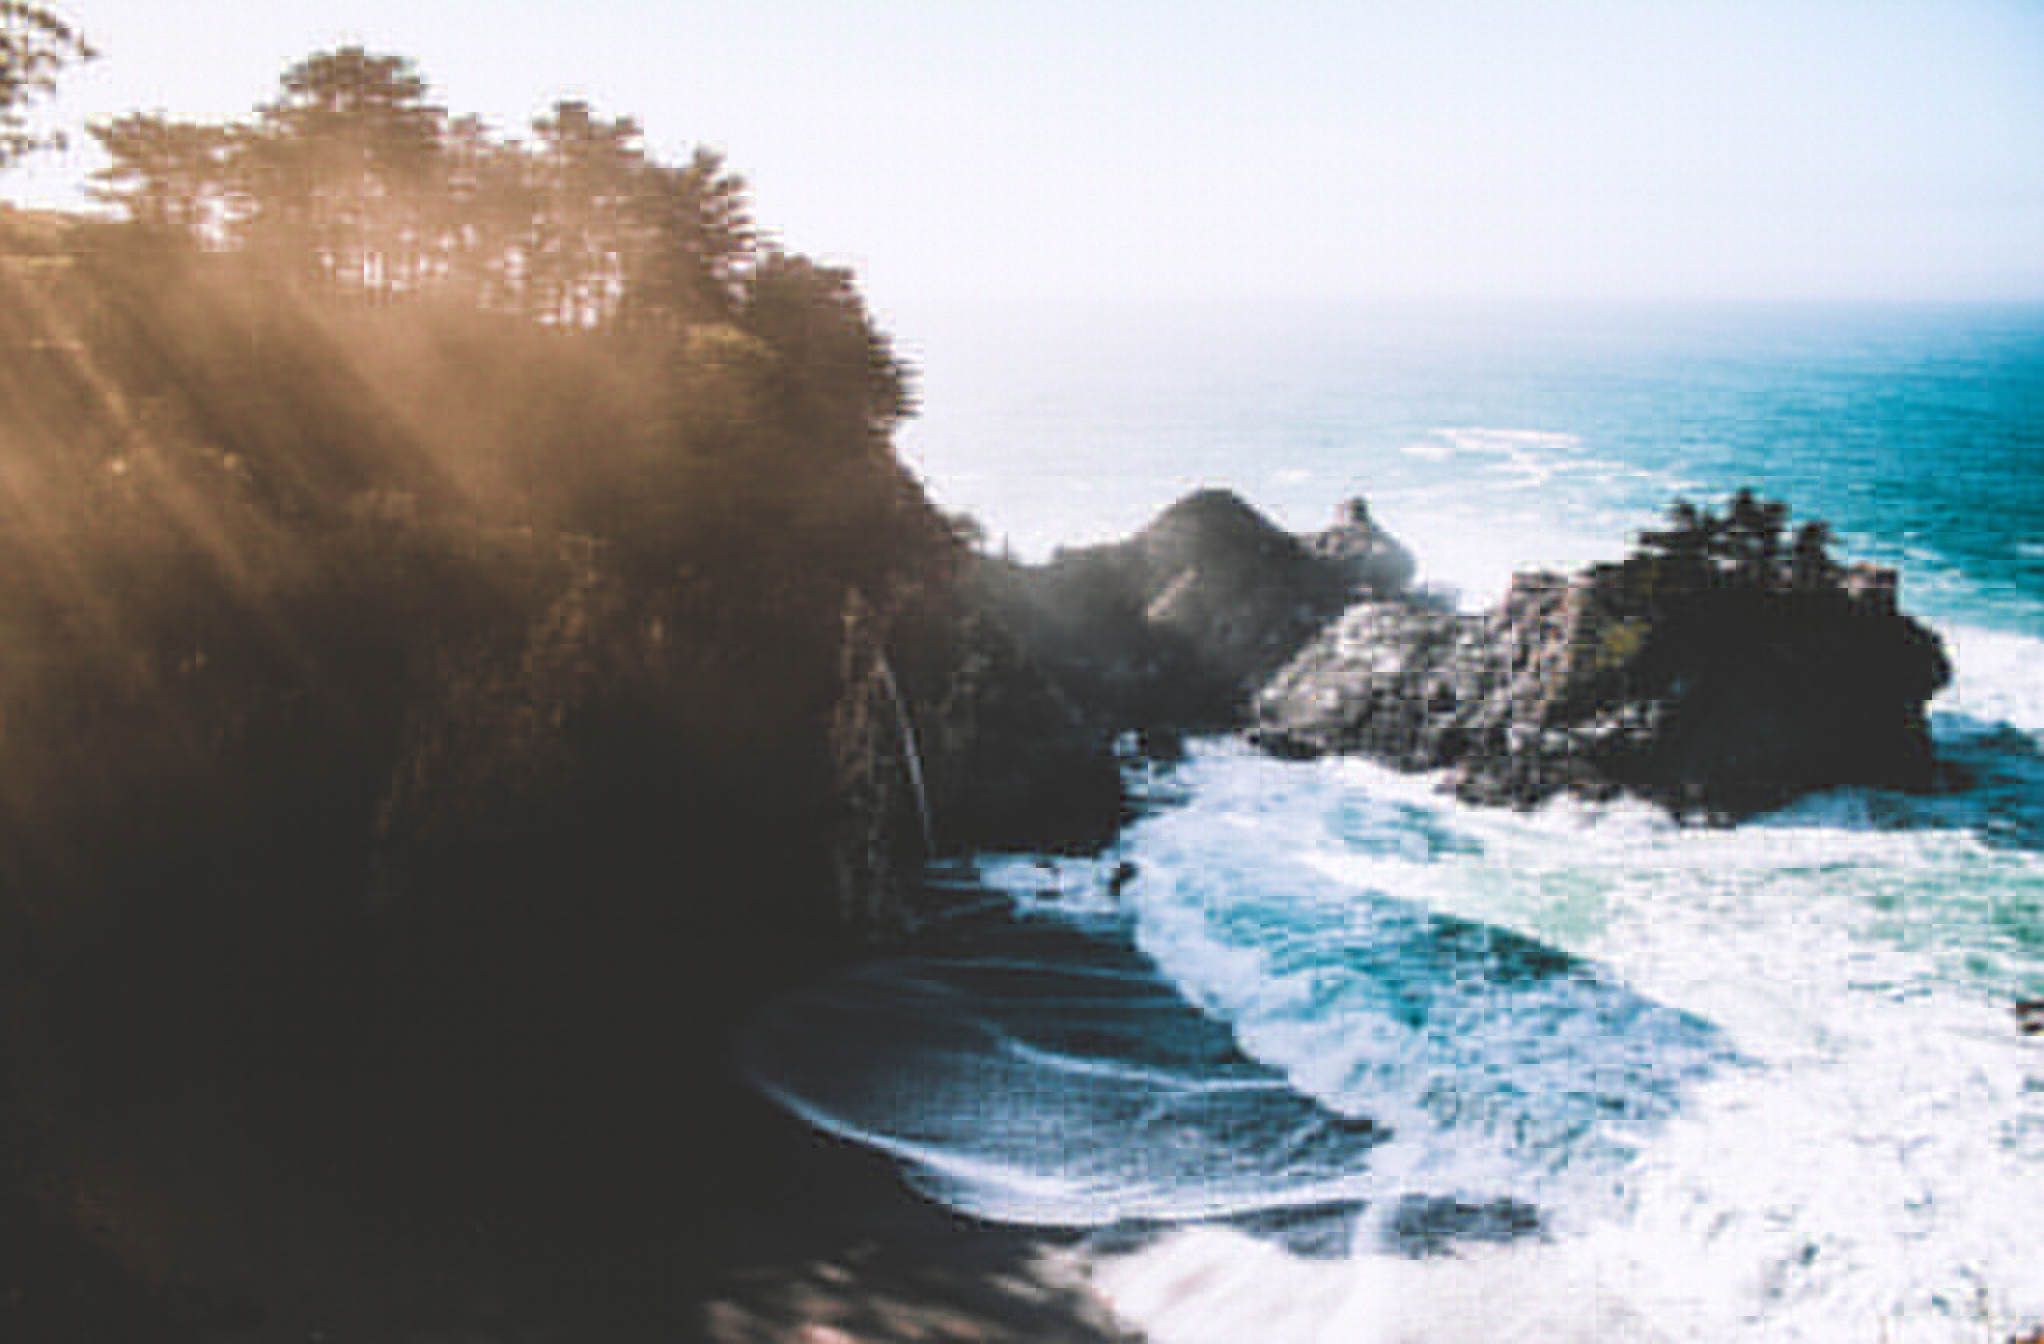
\includegraphics[width=\textwidth]{Images/autoencoder/reconstructed/500/test1_80.png}
    \subcaption{$s=80$}
    \end{subfigure}
    \begin{subfigure}[b]{0.49 \textwidth}
    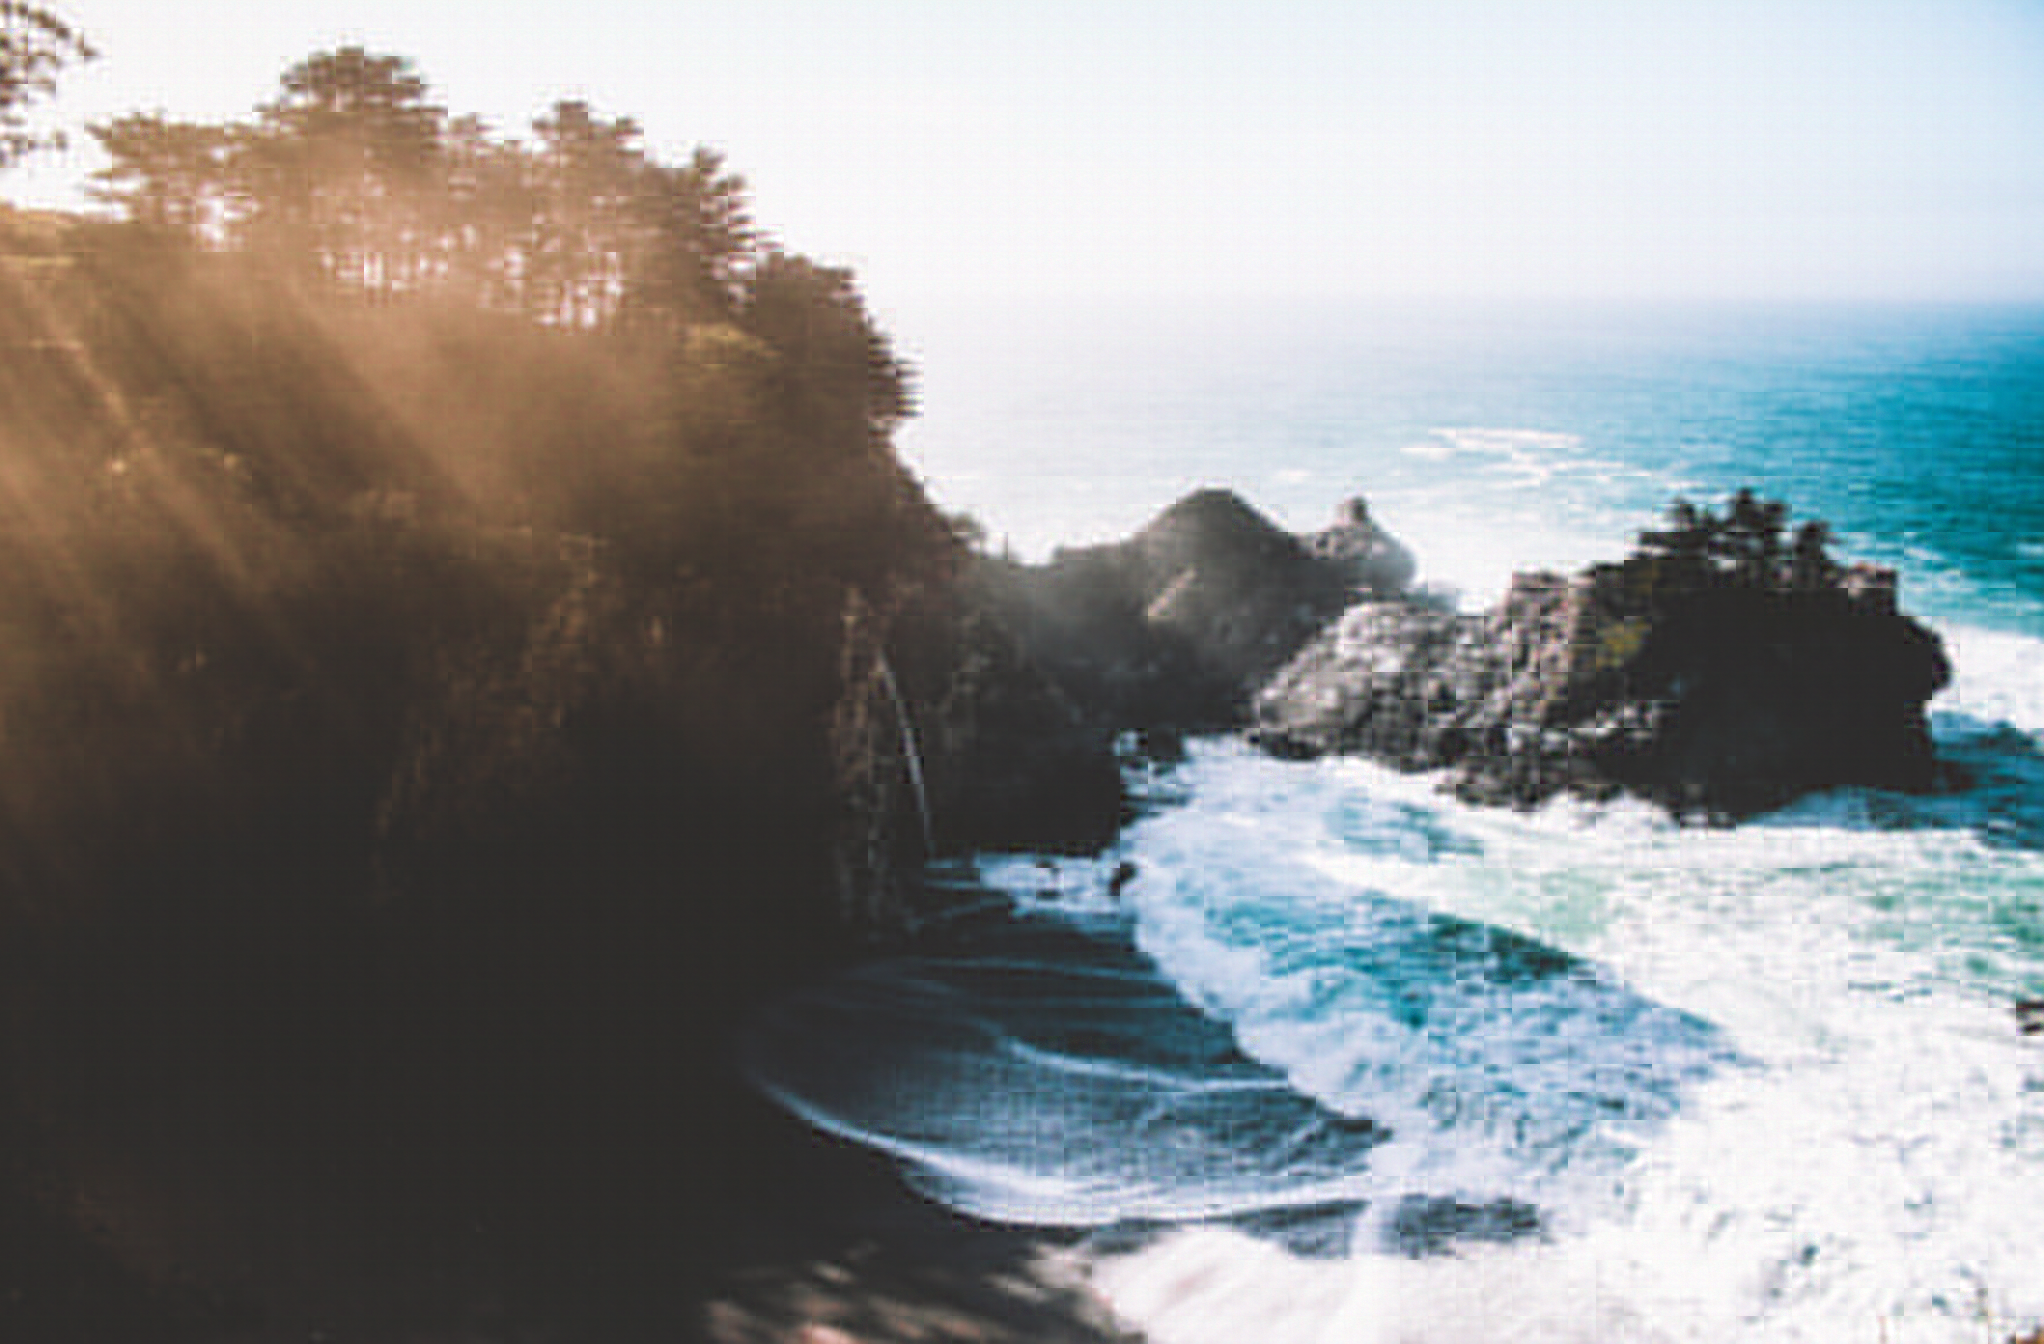
\includegraphics[width=\textwidth]{Images/autoencoder/reconstructed/500/test1_90.png}
    \subcaption{$s=90$}
    \end{subfigure}
    \begin{subfigure}[b]{0.49 \textwidth}
    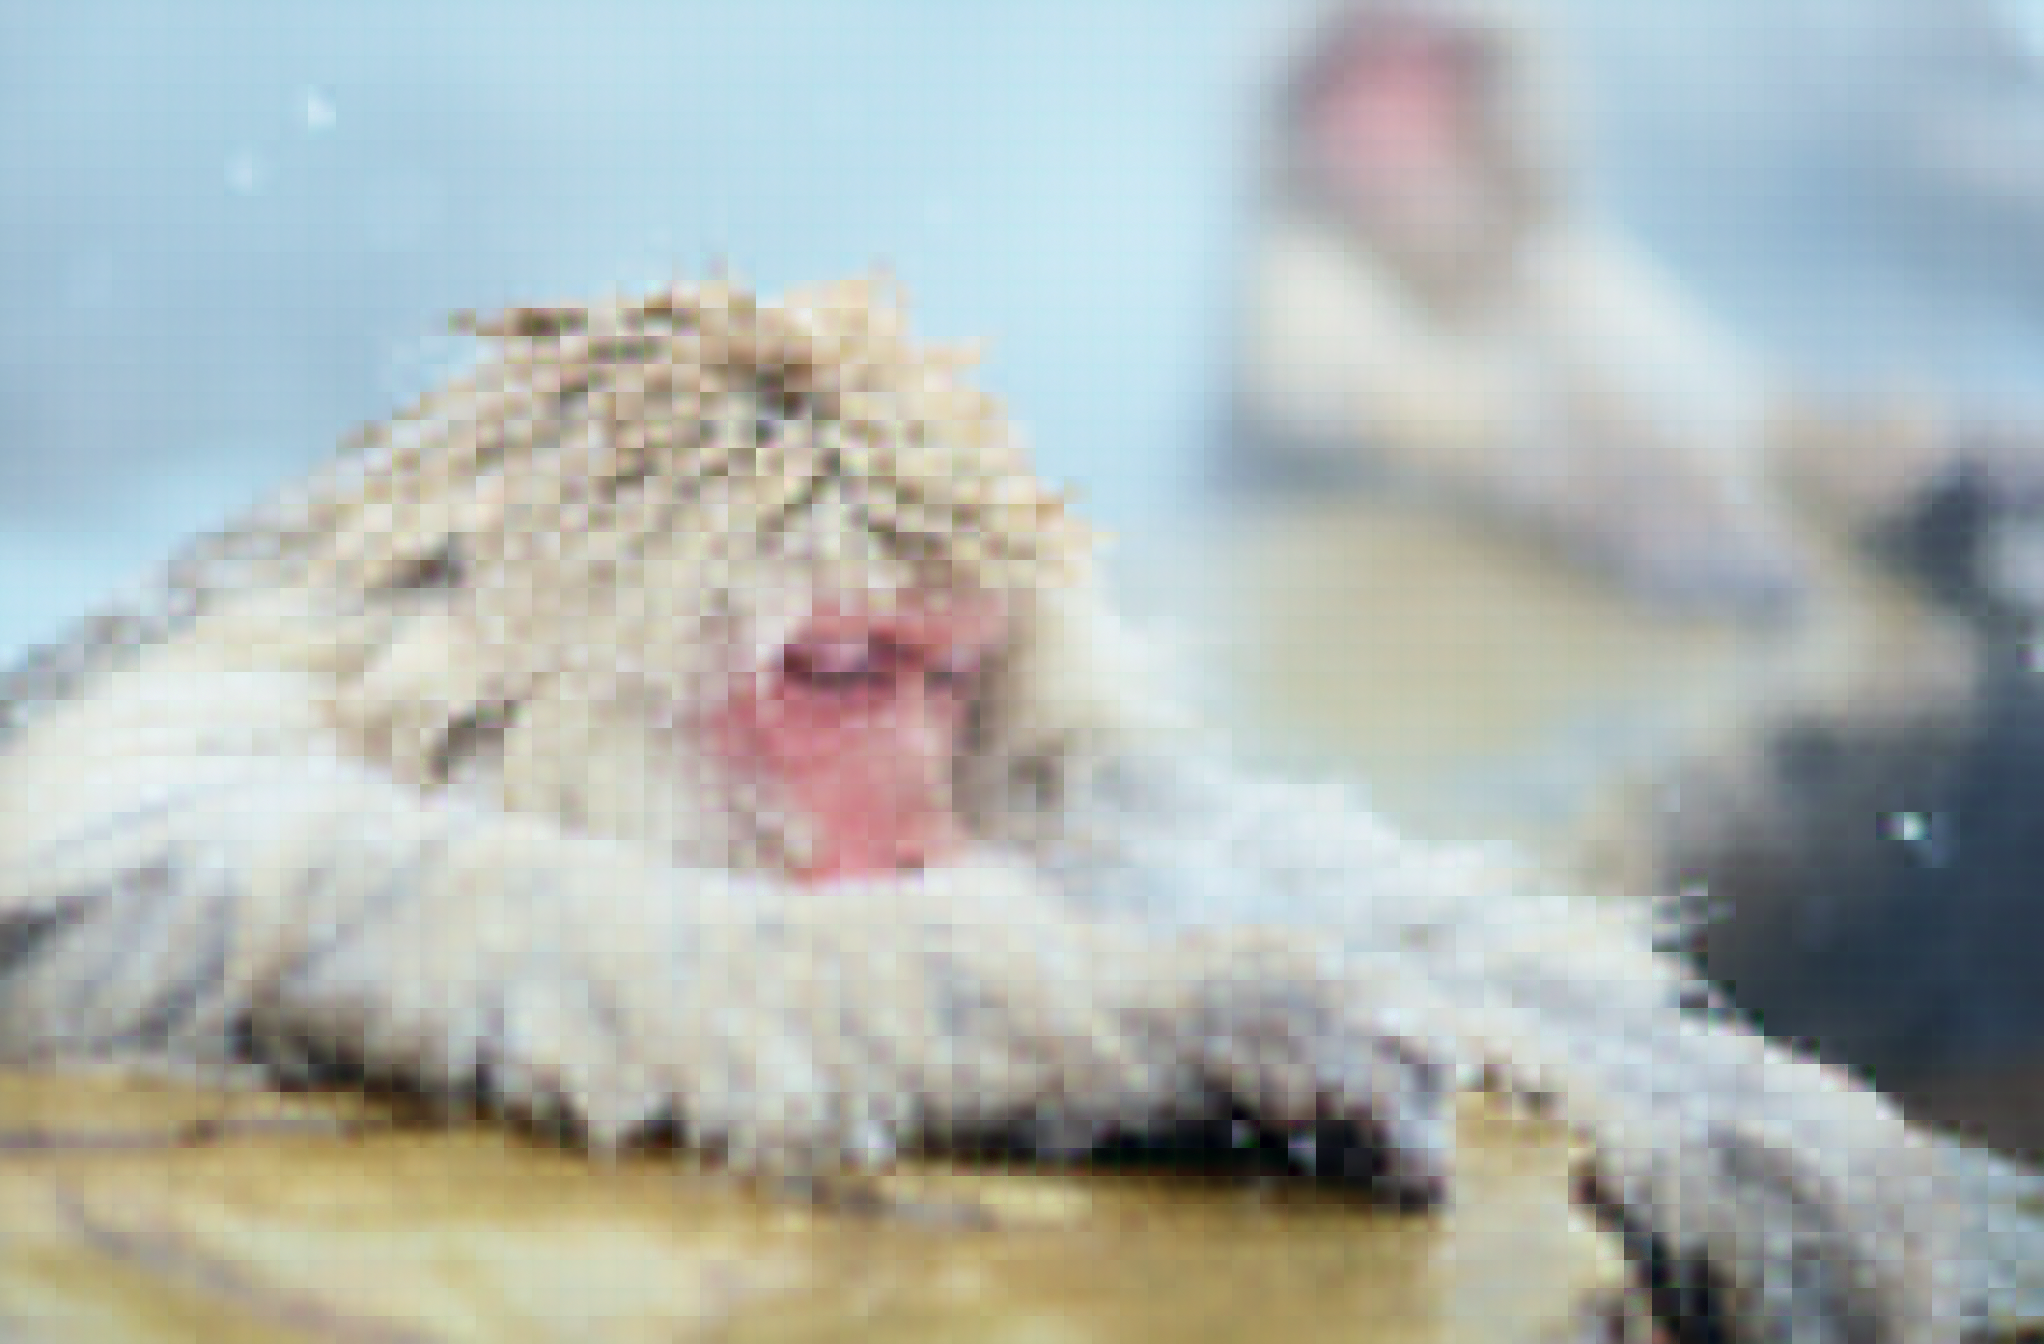
\includegraphics[width=\textwidth]{Images/autoencoder/reconstructed/500/test2_10.png}
    \subcaption{$s=10$}
    \end{subfigure}
    \begin{subfigure}[b]{0.49 \textwidth}
    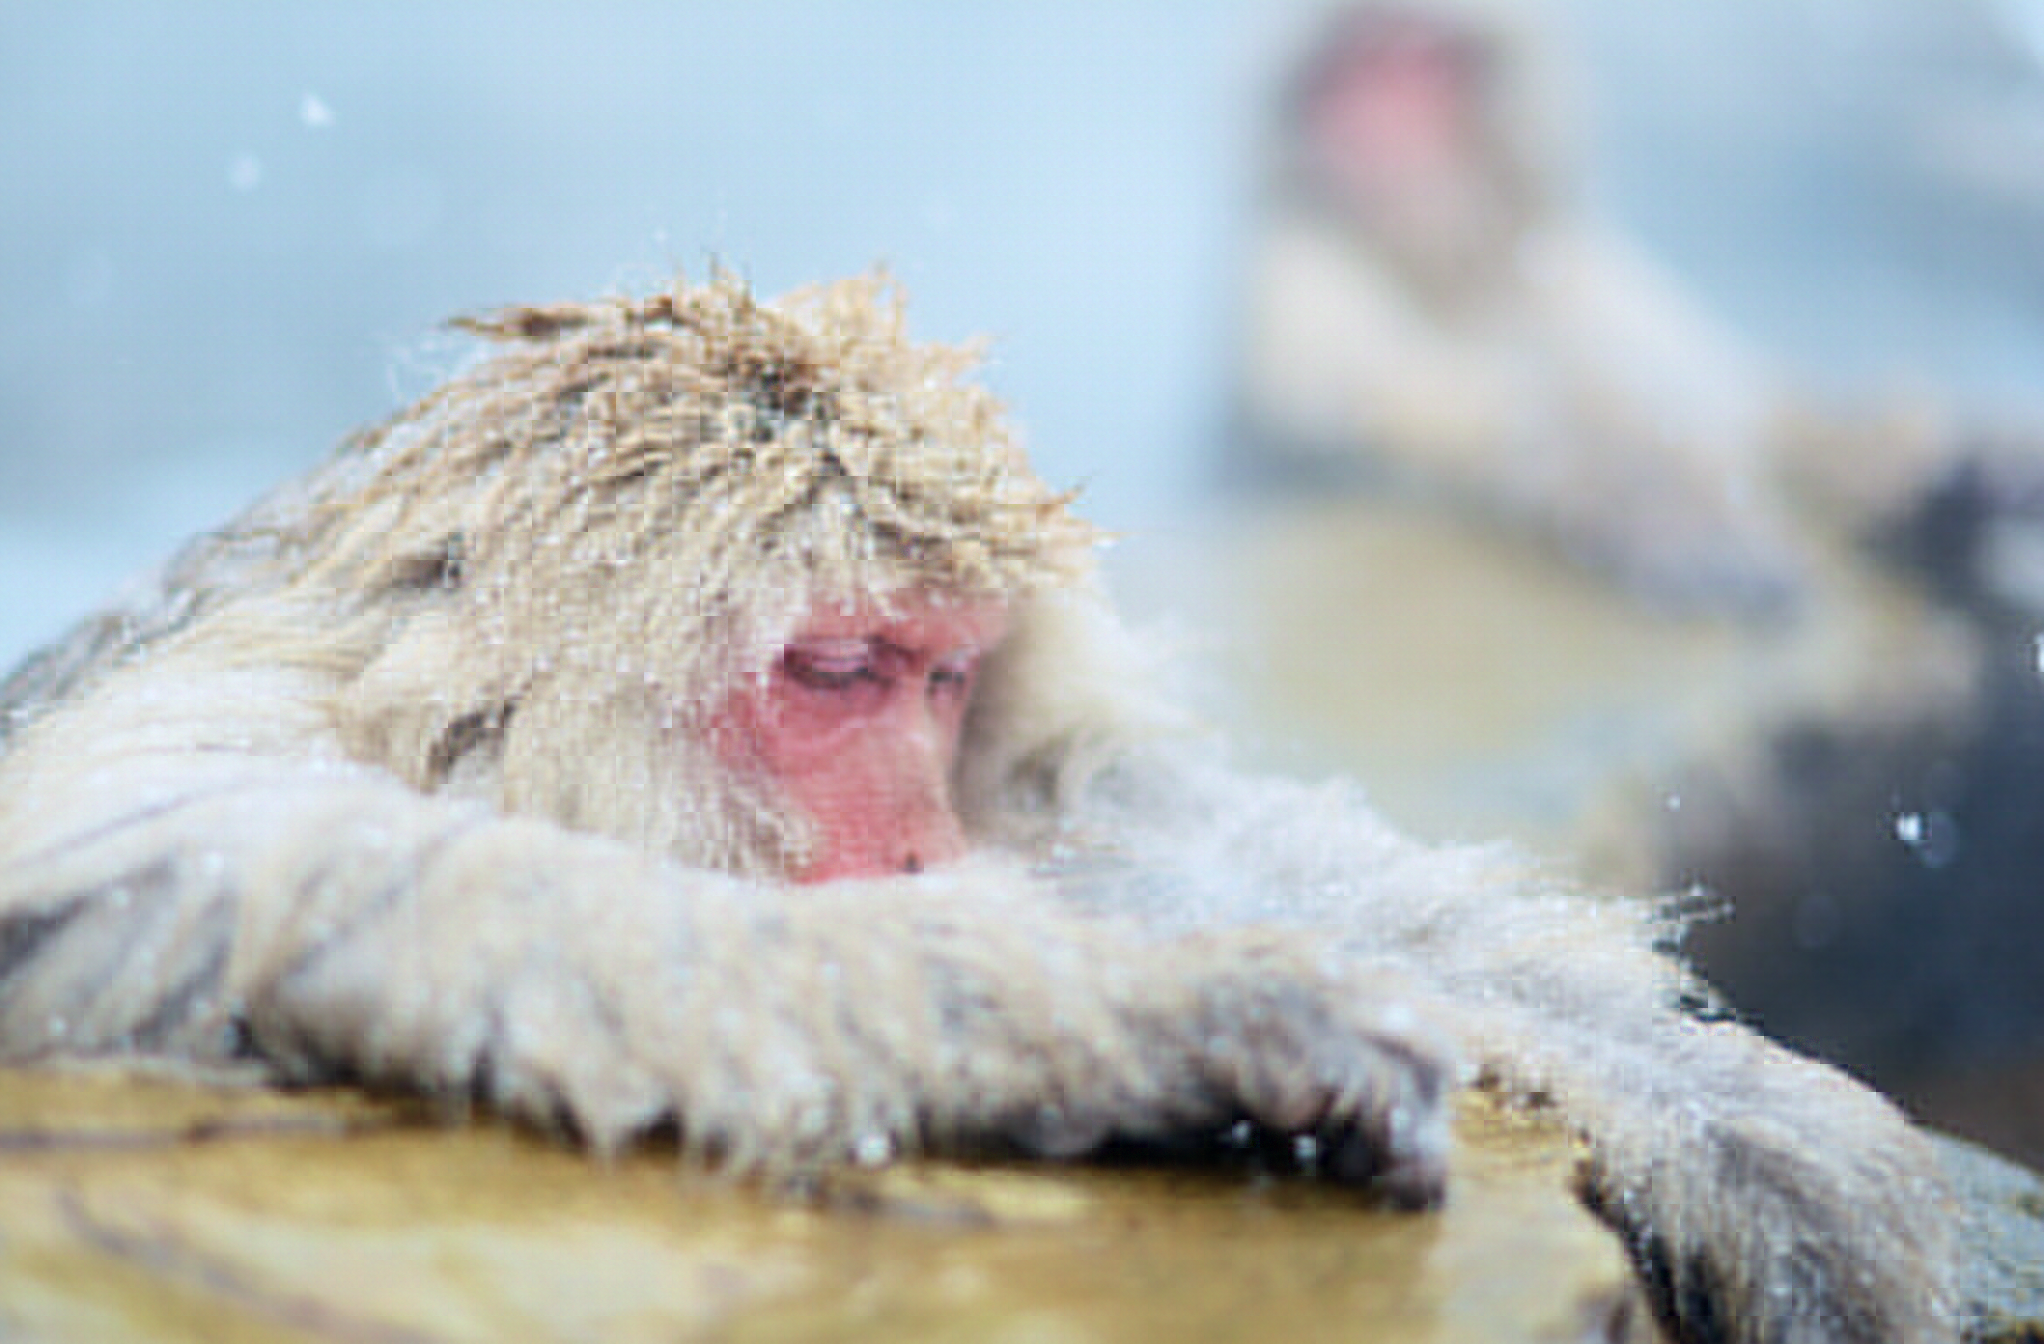
\includegraphics[width=\textwidth]{Images/autoencoder/reconstructed/500/test2_80.png}
    \subcaption{$s=80$}
    \end{subfigure}
    \begin{subfigure}[b]{0.49 \textwidth}
    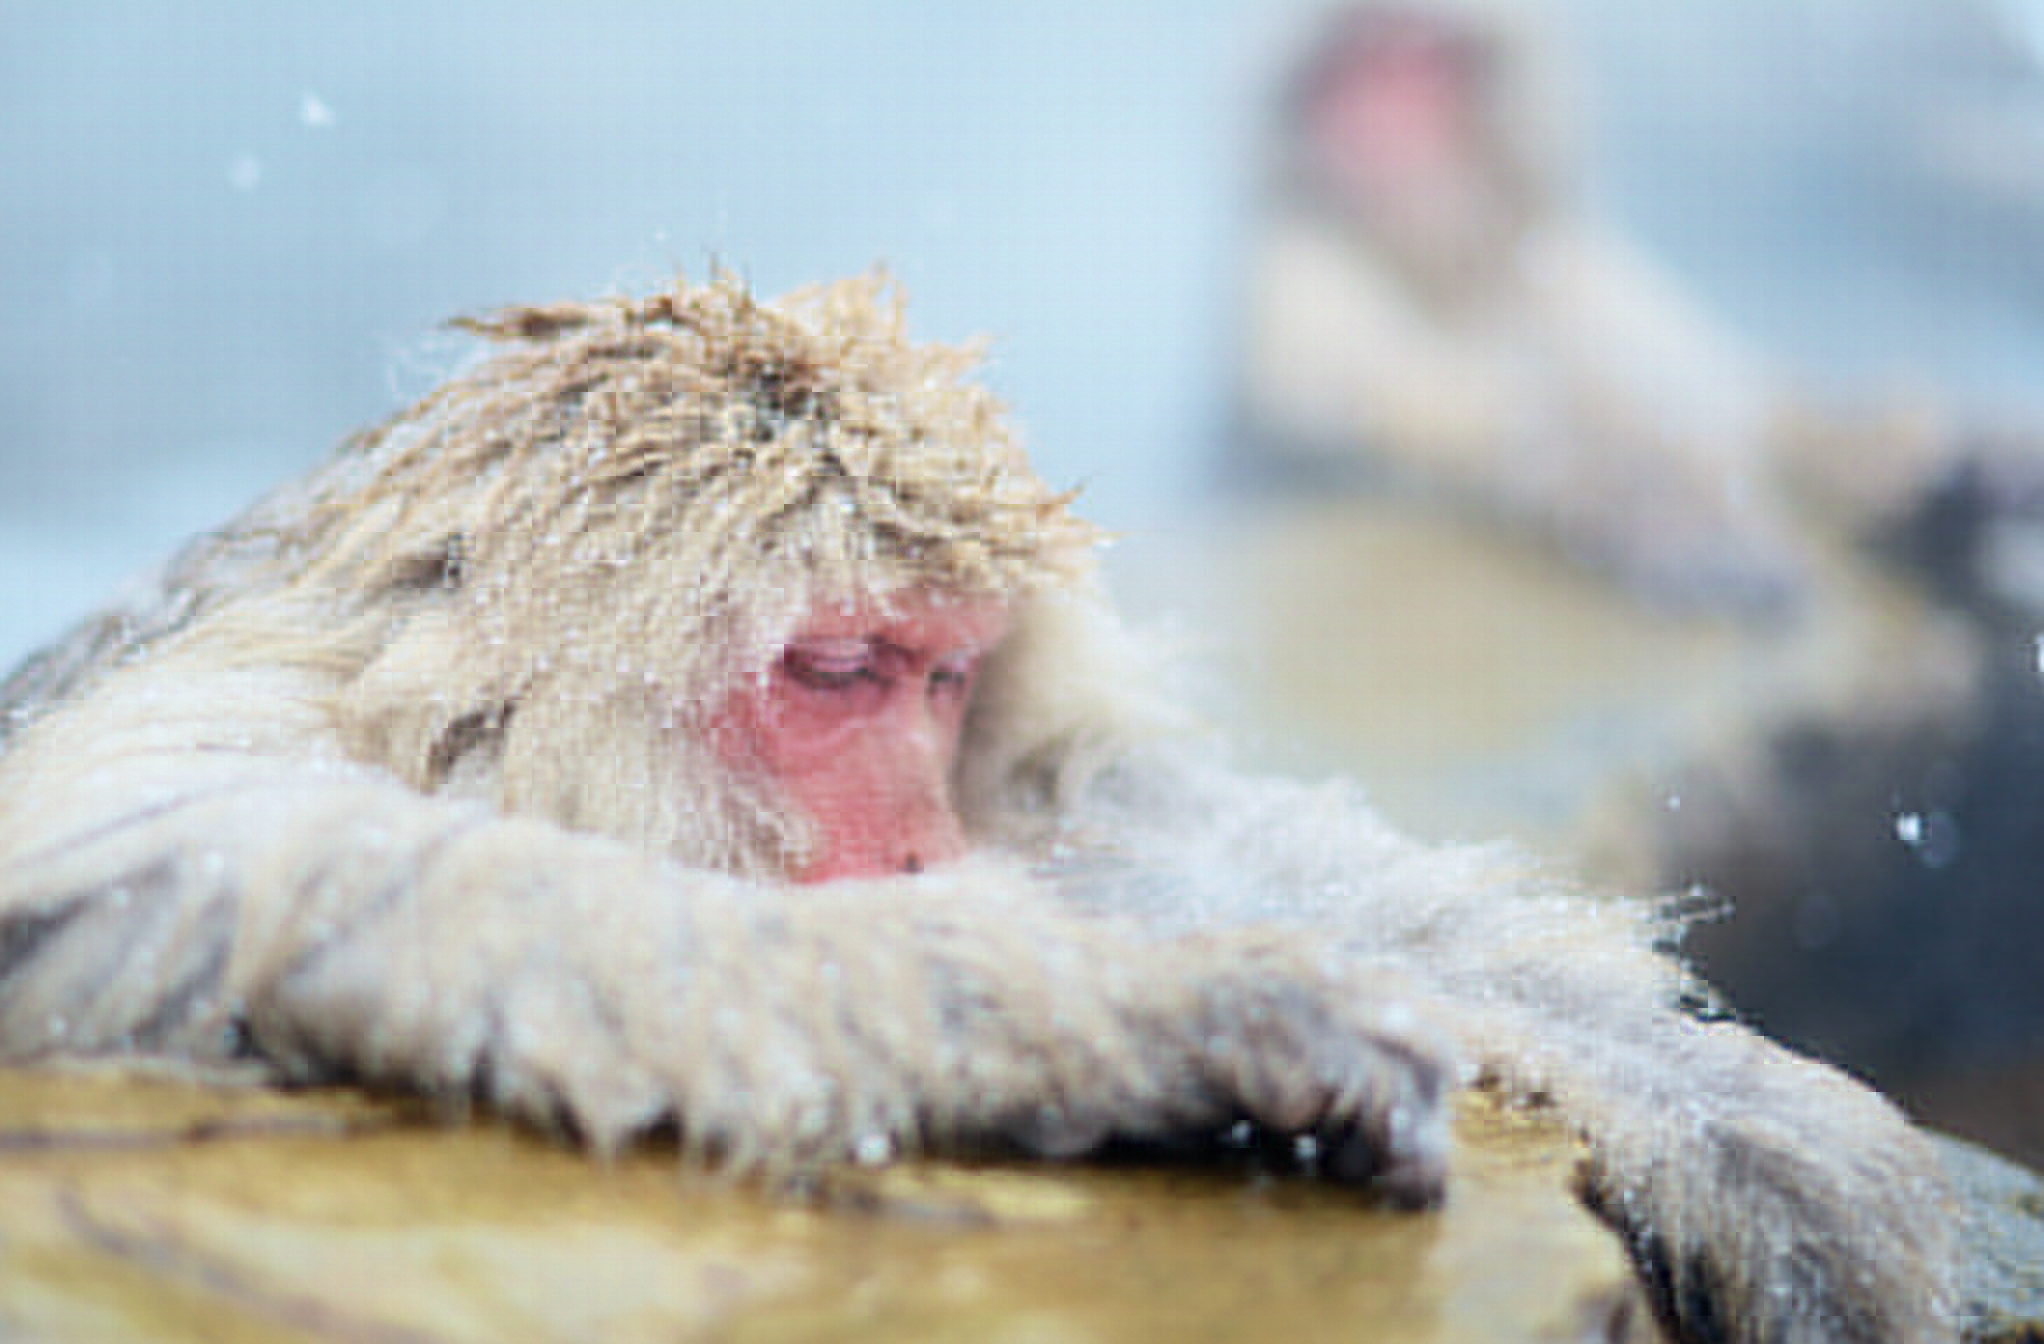
\includegraphics[width=\textwidth]{Images/autoencoder/reconstructed/500/test2_90.png}
    \subcaption{$s=90$}
    \end{subfigure}
\end{figure}

\begin{figure}
\ContinuedFloat
    \begin{subfigure}[b]{0.49 \textwidth}
    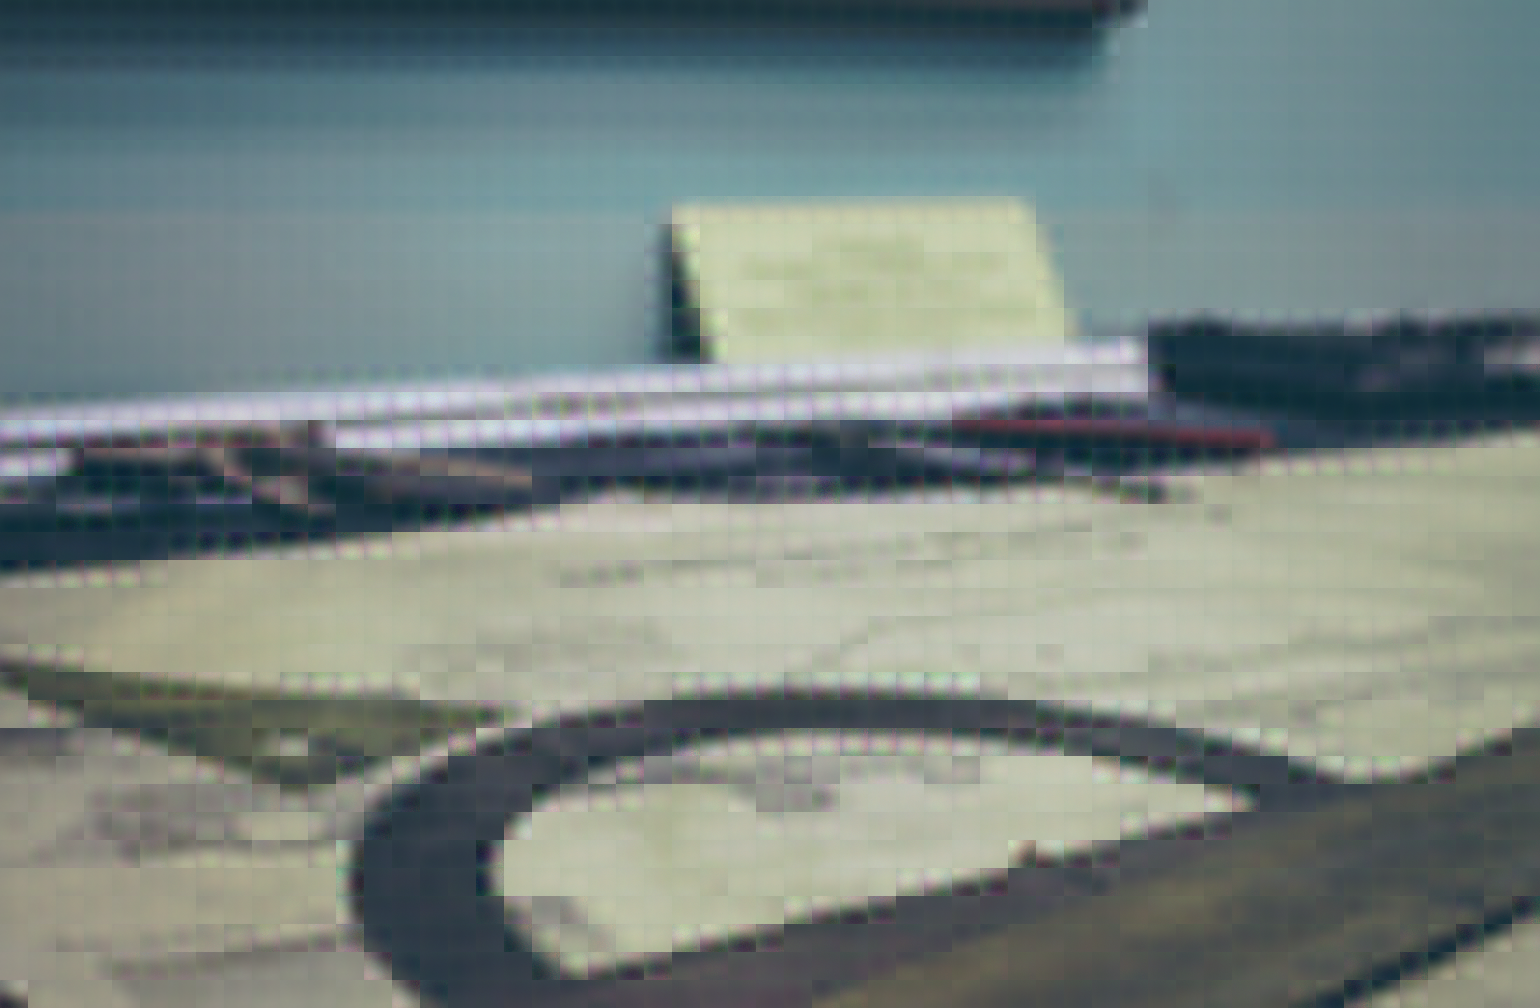
\includegraphics[width=\textwidth]{Images/autoencoder/reconstructed/500/test3_10.png}
    \subcaption{$s=10$}
    \end{subfigure}
    \begin{subfigure}[b]{0.49 \textwidth}
    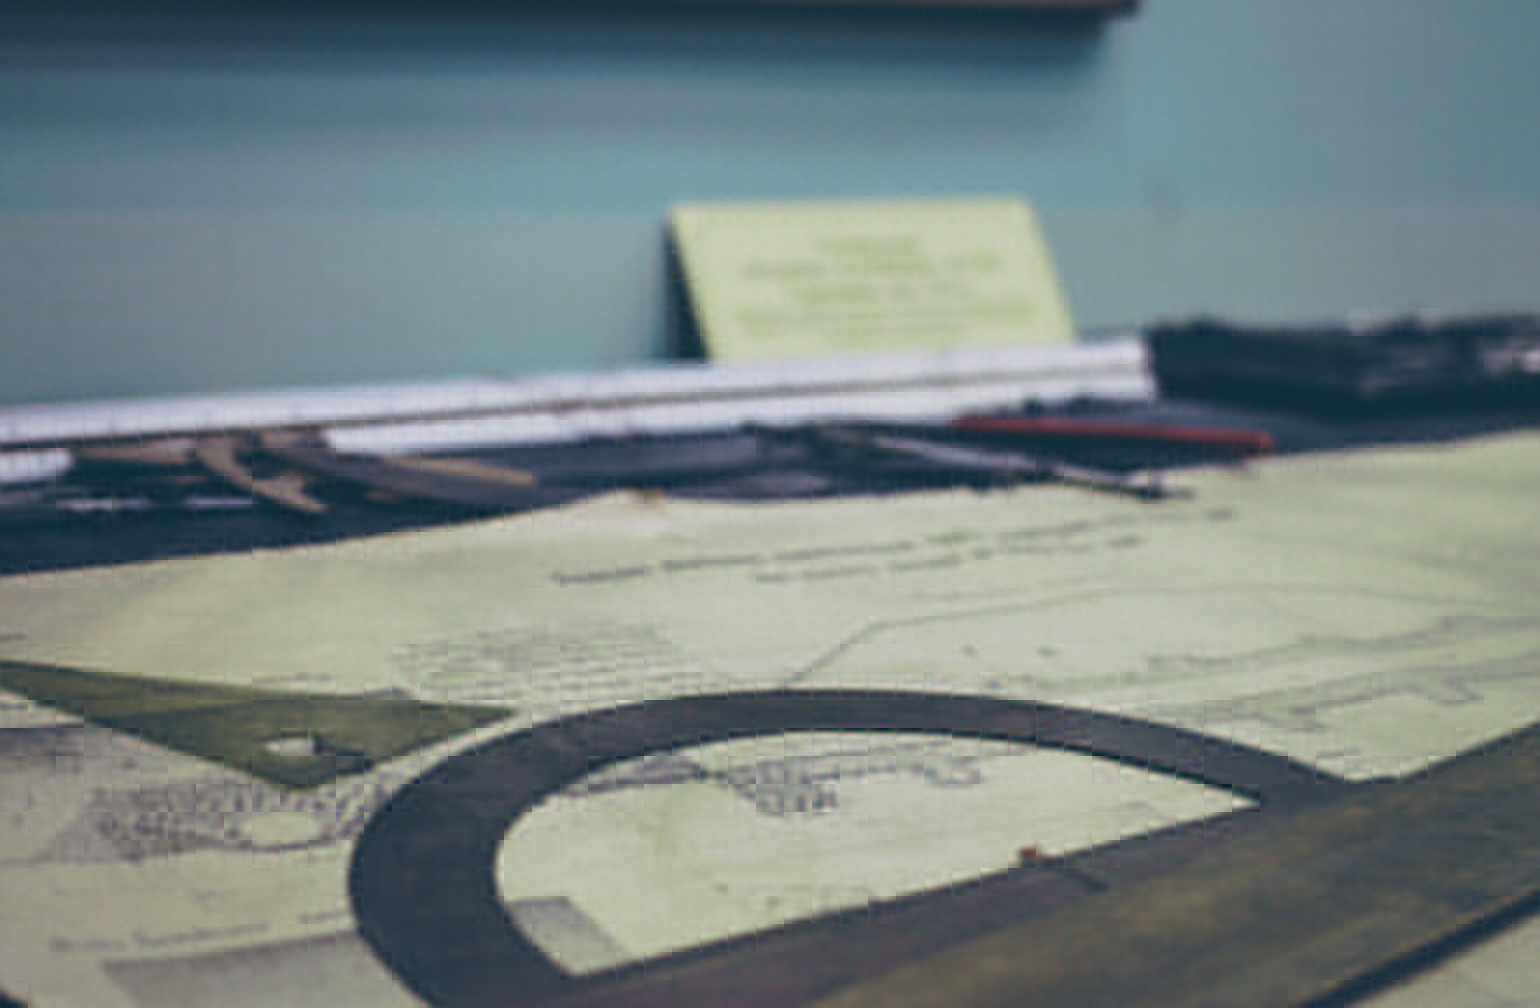
\includegraphics[width=\textwidth]{Images/autoencoder/reconstructed/500/test3_80.png}
    \subcaption{$s=80$}
    \end{subfigure}
    \begin{subfigure}[b]{0.49 \textwidth}
    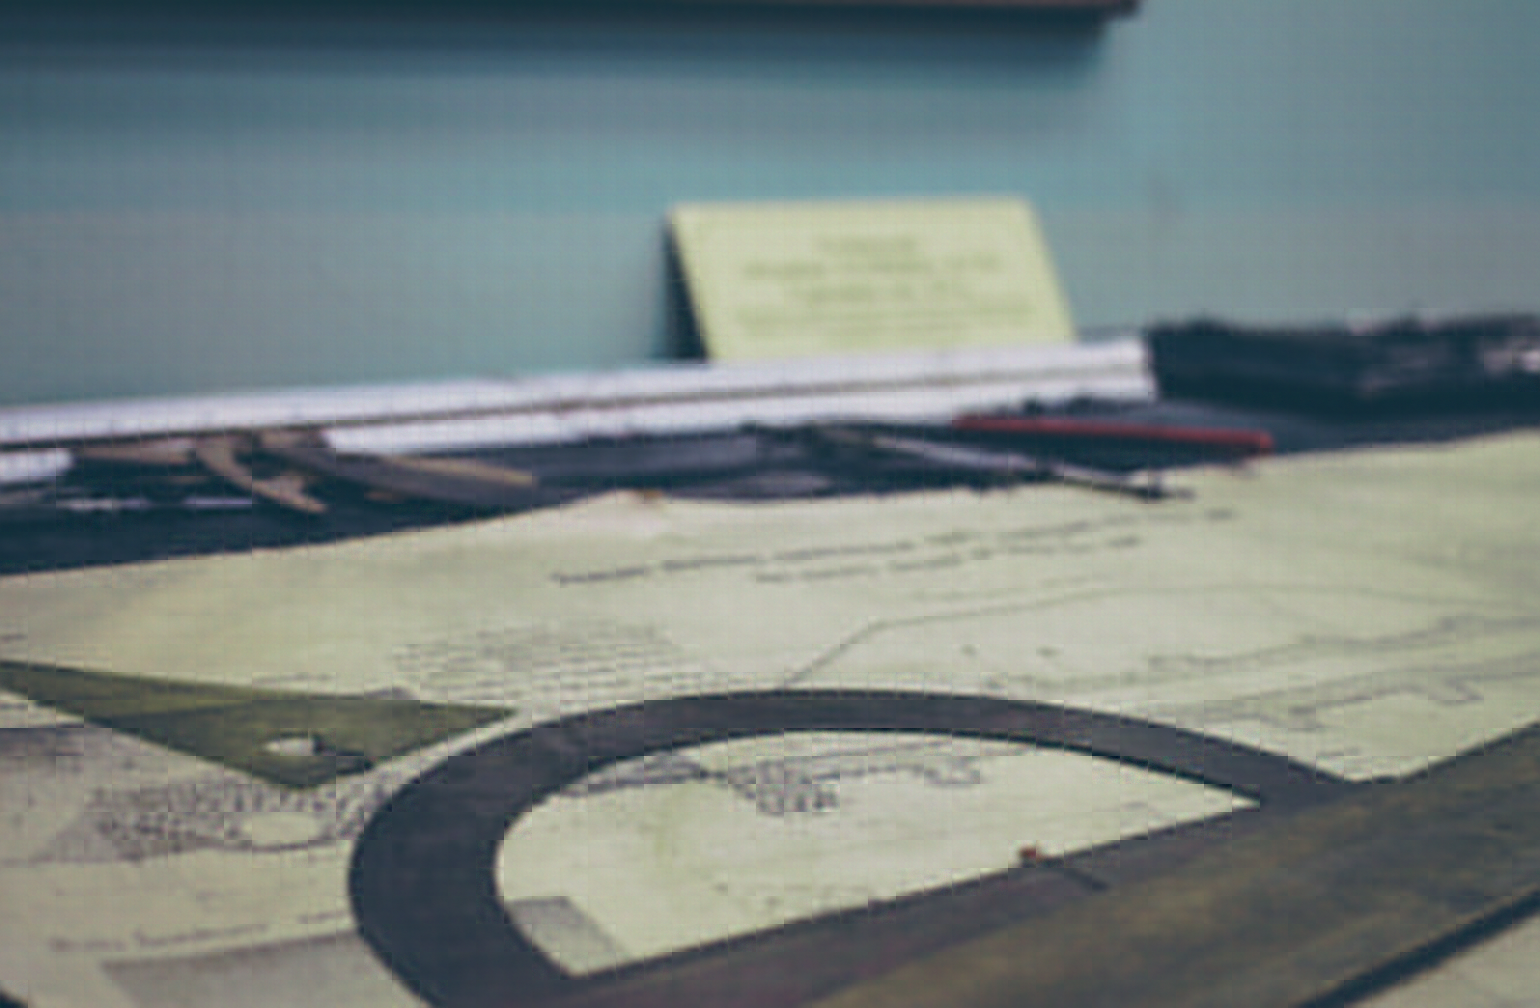
\includegraphics[width=\textwidth]{Images/autoencoder/reconstructed/500/test3_90.png}
    \subcaption{$s=90$}
    \end{subfigure}
    \caption{Output of auto-encoder when using reference architecture and varying the size of the latent space.}
    \label{fig:auto_latent}
\end{figure}

This was followed by modifying the depth of the network, i.e. changing the size of the first hidden layer to $512$ and adding a second hidden layer of size $256$ and a third layer of $128$. The sizes was adapted to be a power of $2$ since this is mostly used in literature (although there is no proof for faster convergence or similar). No more hidden layers were added because going even smaller would create a layer having a size smaller than the latent space. The respective results for a two-layer and a three-layer network can be seen in Figure \ref{fig:auto_layers}. We can observe that while keeping all configurations the same (apart from the number of epochs which were increased to achieve convergence) and increasing the depth of the network, the output of the decoder becomes more and more aliased.\\

\begin{figure}
    \centering
    \begin{subfigure}[b]{0.49 \textwidth}
    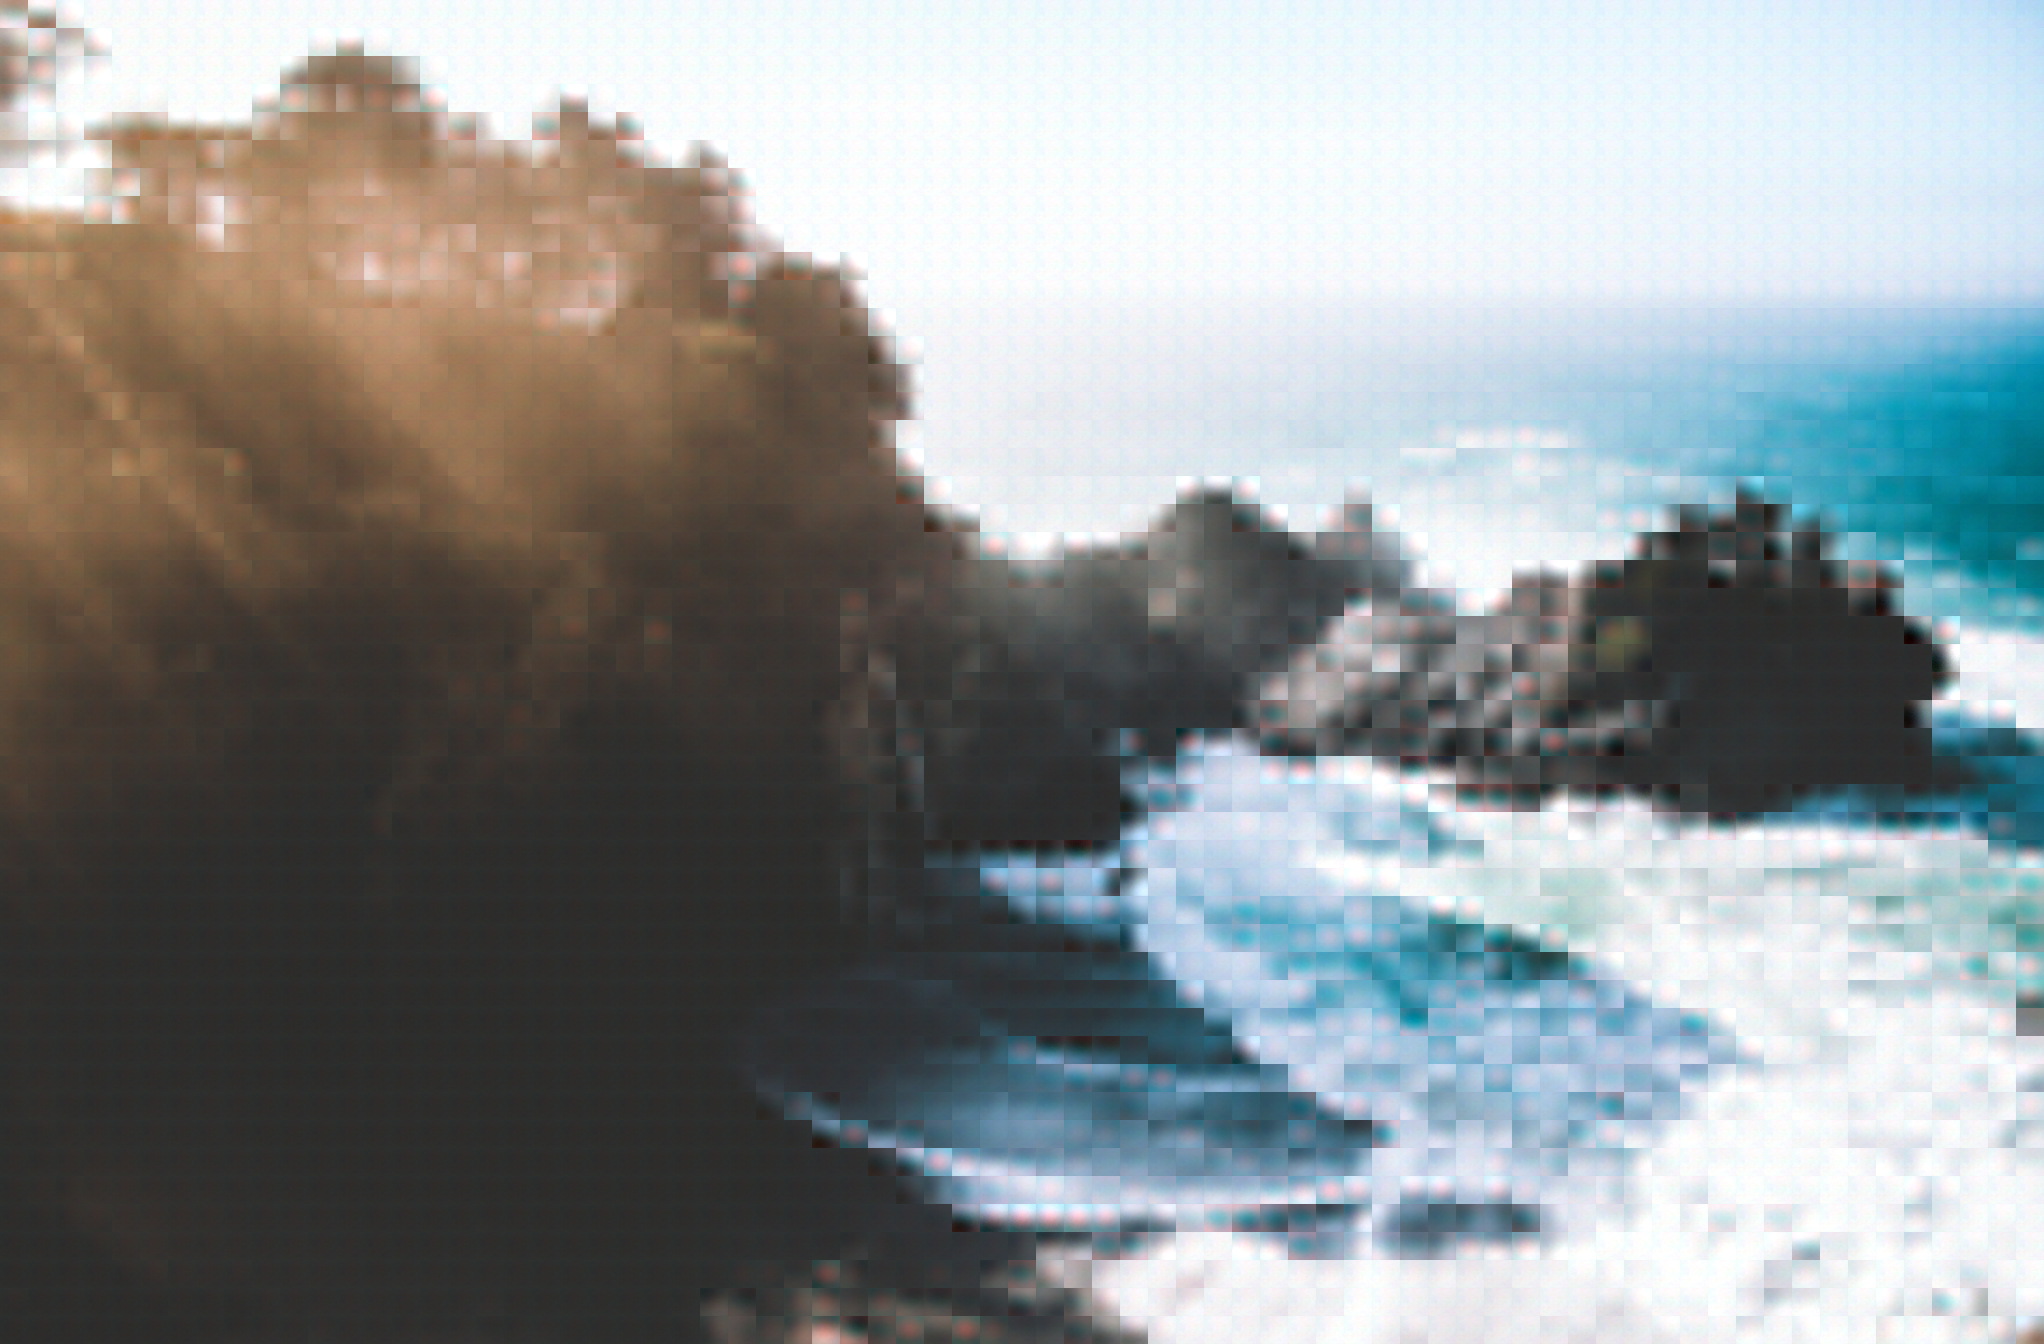
\includegraphics[width=\textwidth]{Images/autoencoder/reconstructed/512_256/test1_80.png}
    \subcaption{(512, 256)}
    \end{subfigure}
    \begin{subfigure}[b]{0.49 \textwidth}
    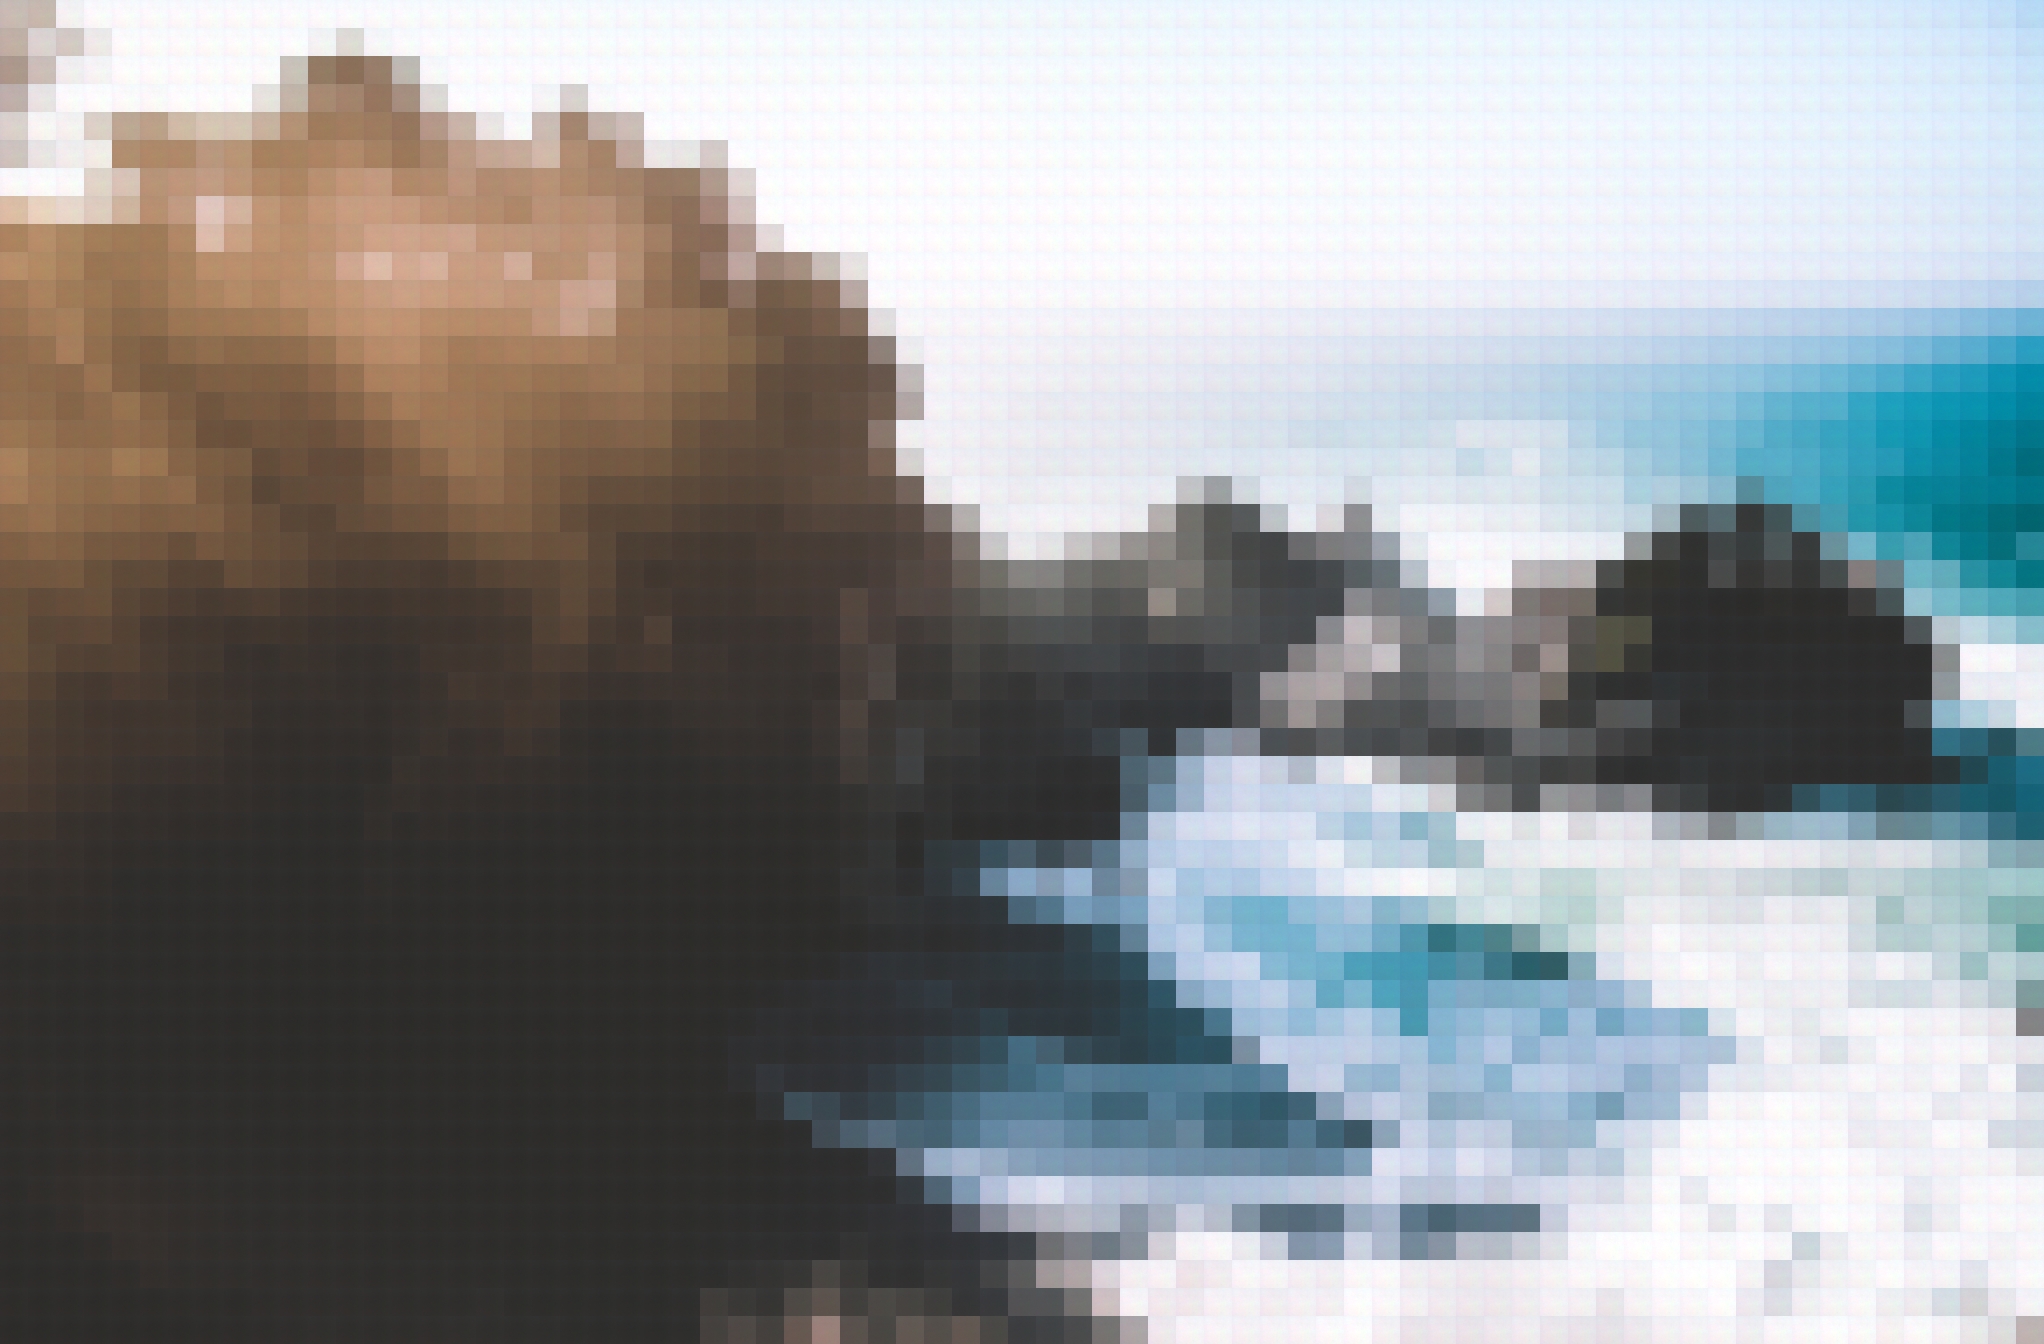
\includegraphics[width=\textwidth]{Images/autoencoder/reconstructed/512_256_128/test1_80.png}
    \subcaption{(512, 256, 128)}
    \end{subfigure}
    \begin{subfigure}[b]{0.49 \textwidth}
    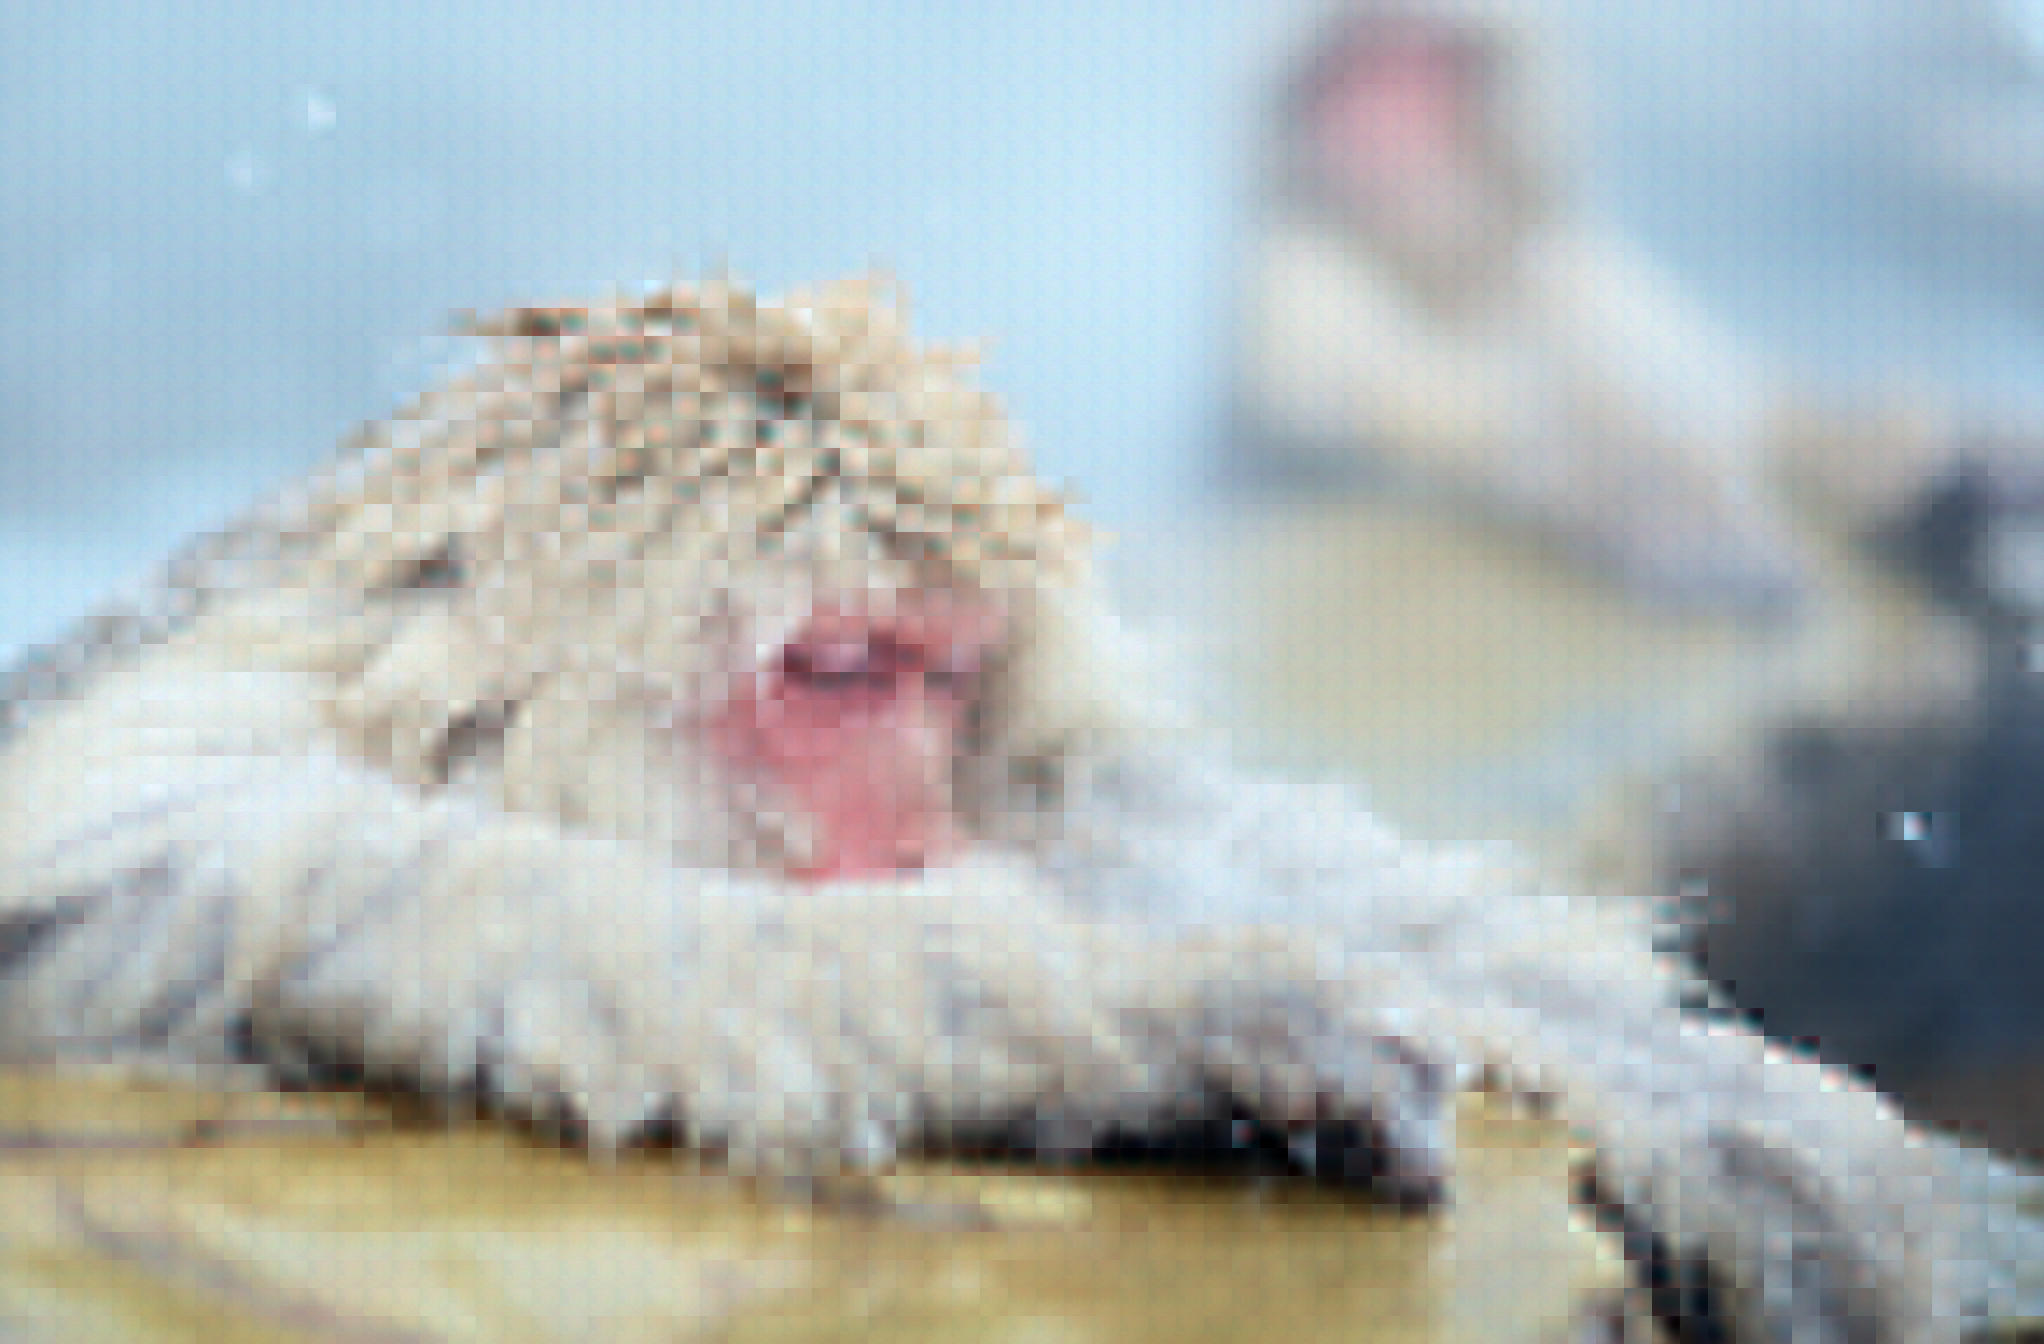
\includegraphics[width=\textwidth]{Images/autoencoder/reconstructed/512_256/test2_80.png}
    \subcaption{(512, 256)}
    \end{subfigure}
    \begin{subfigure}[b]{0.49 \textwidth}
    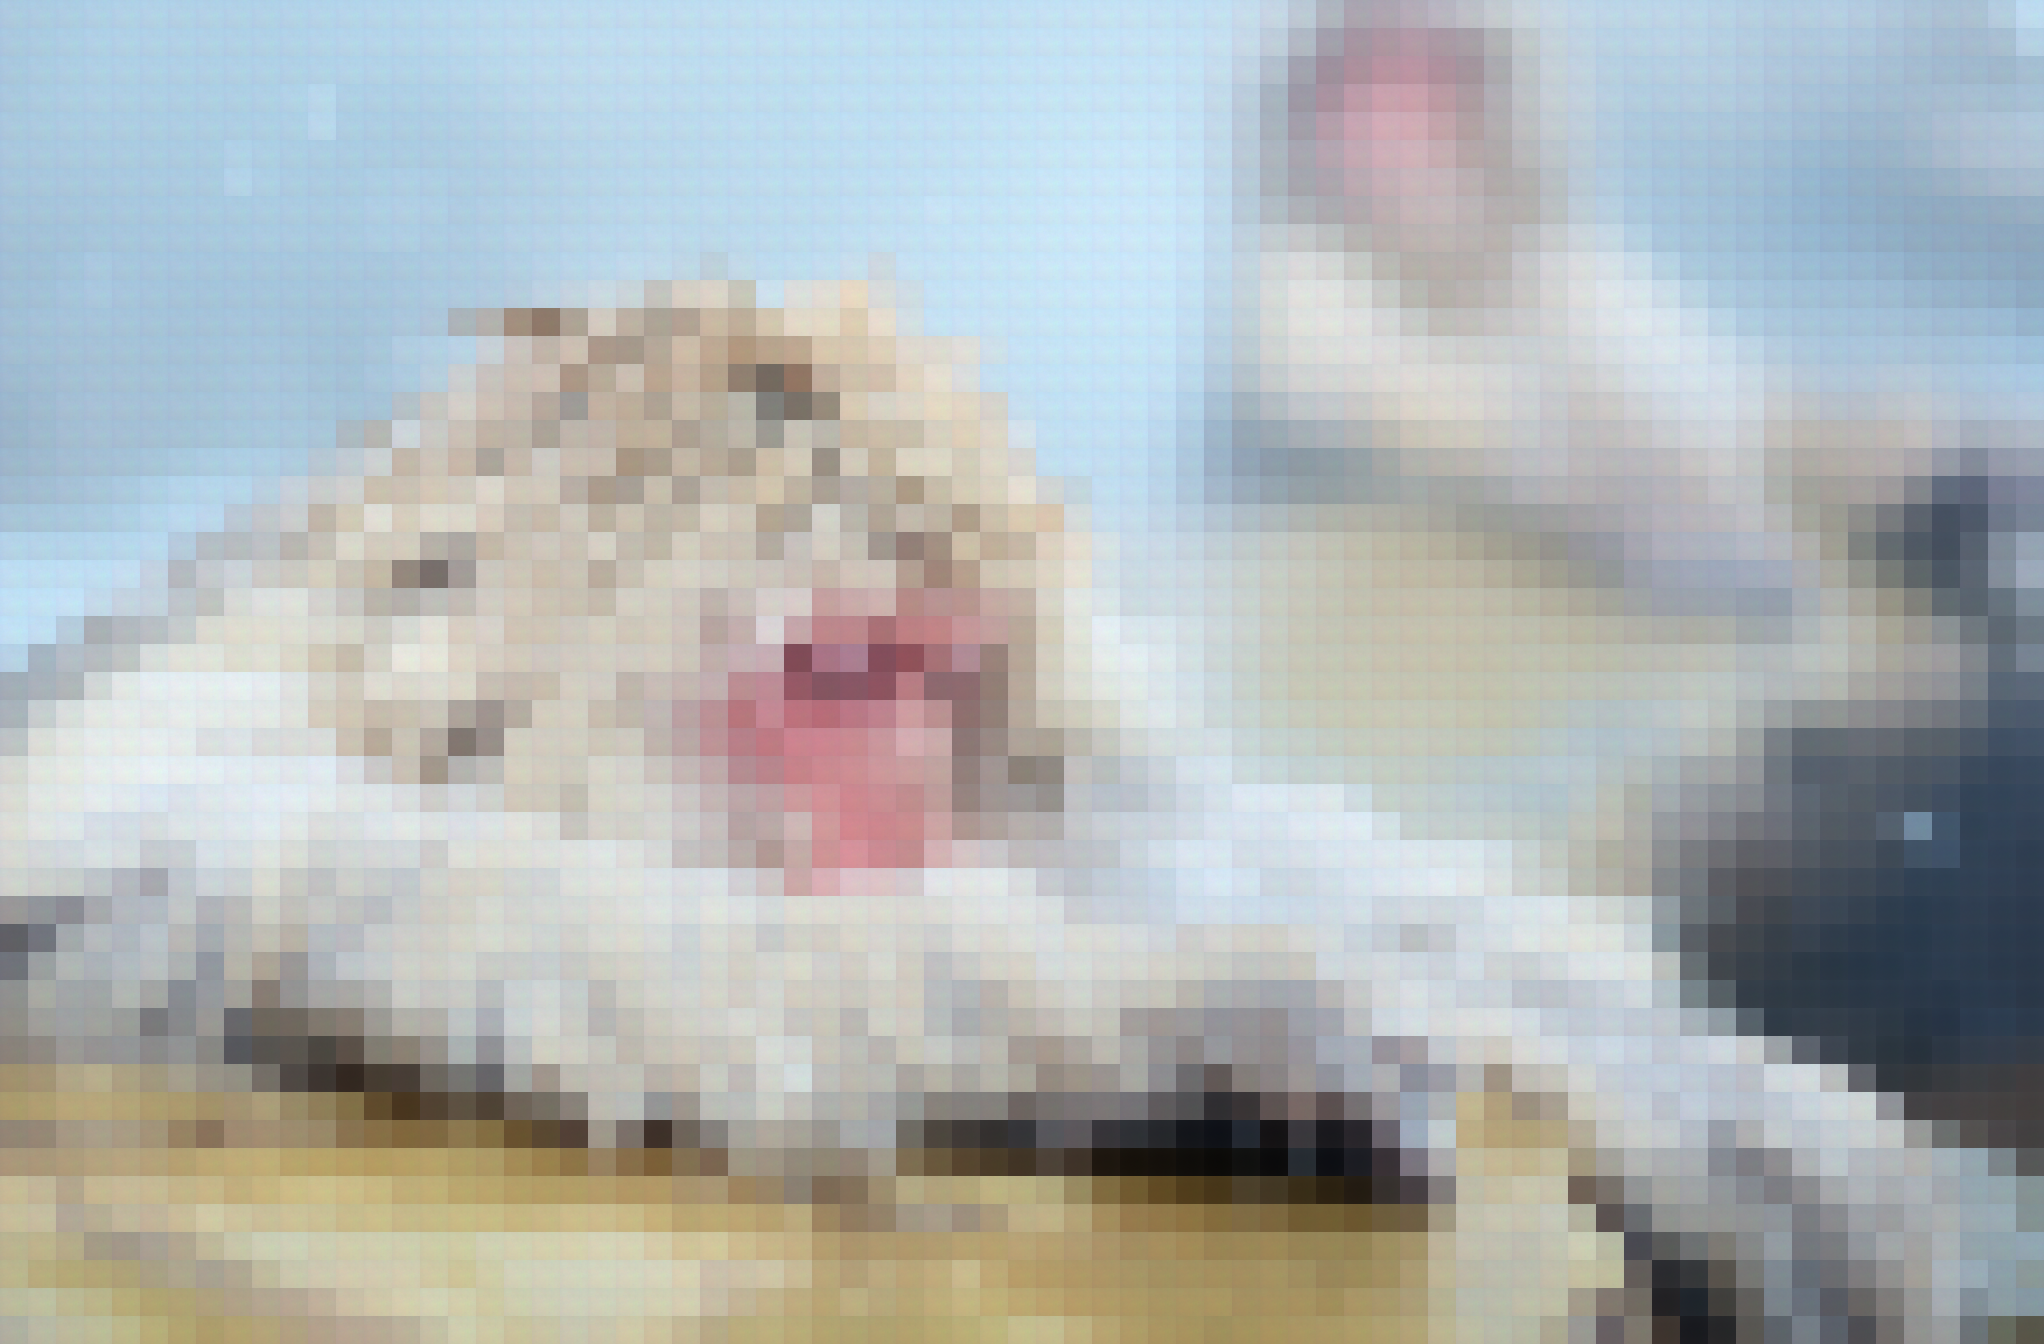
\includegraphics[width=\textwidth]{Images/autoencoder/reconstructed/512_256_128/test2_80.png}
    \subcaption{(512, 256, 128)}
    \end{subfigure}
    \begin{subfigure}[b]{0.49 \textwidth}
    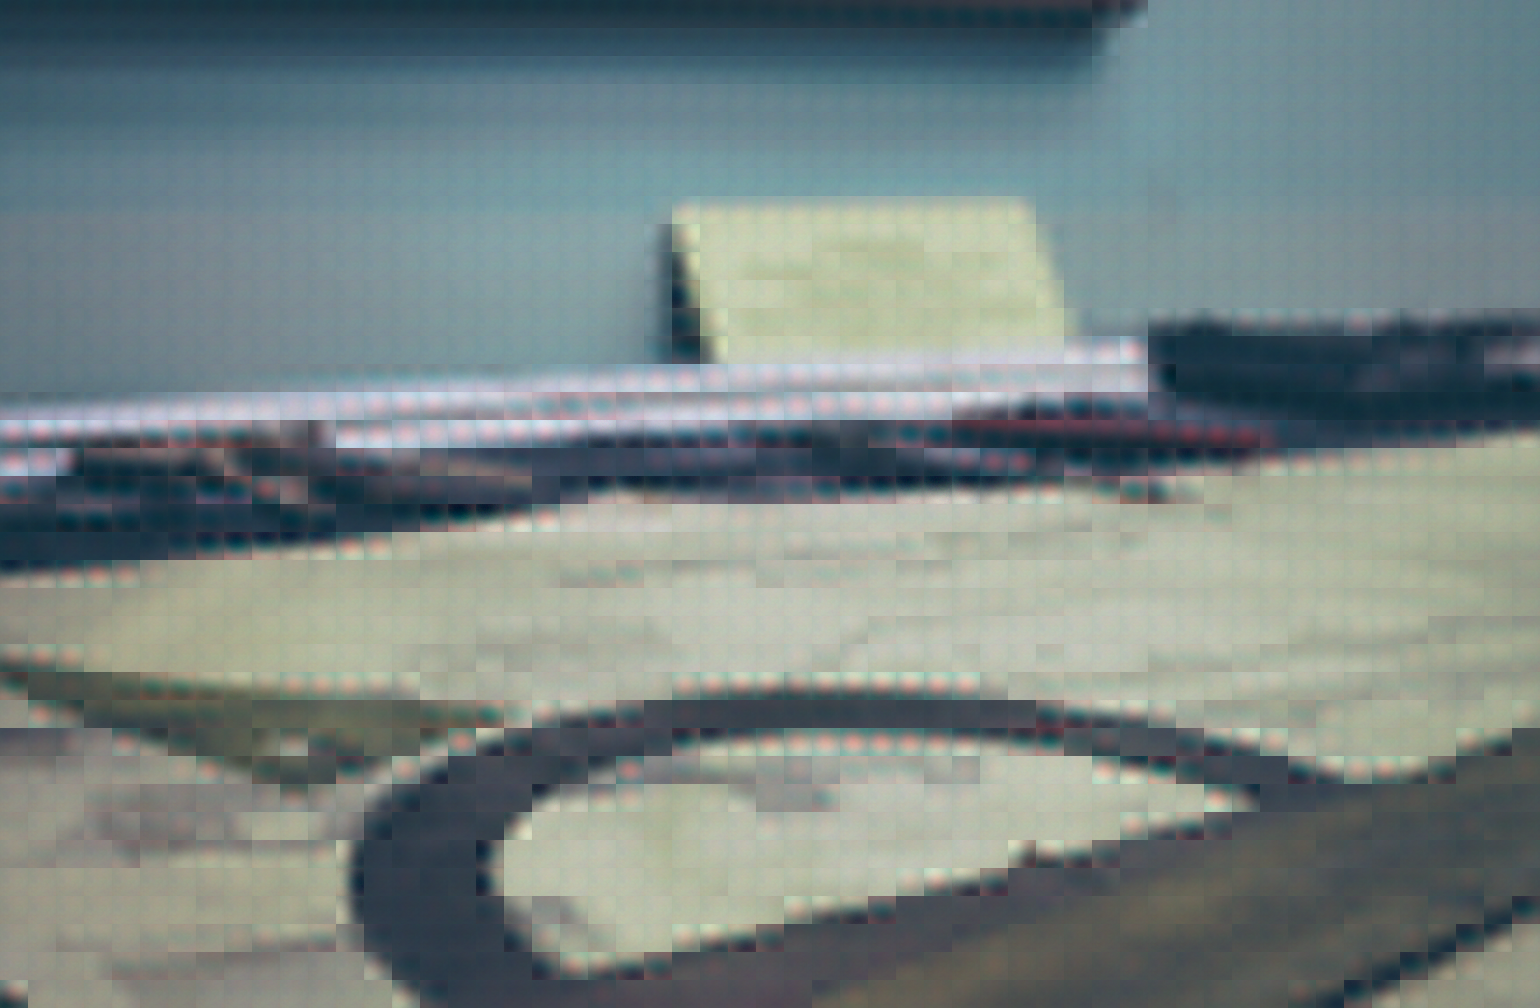
\includegraphics[width=\textwidth]{Images/autoencoder/reconstructed/512_256/test3_80.png}
    \subcaption{(512, 256)}
    \end{subfigure}
    \begin{subfigure}[b]{0.49 \textwidth}
    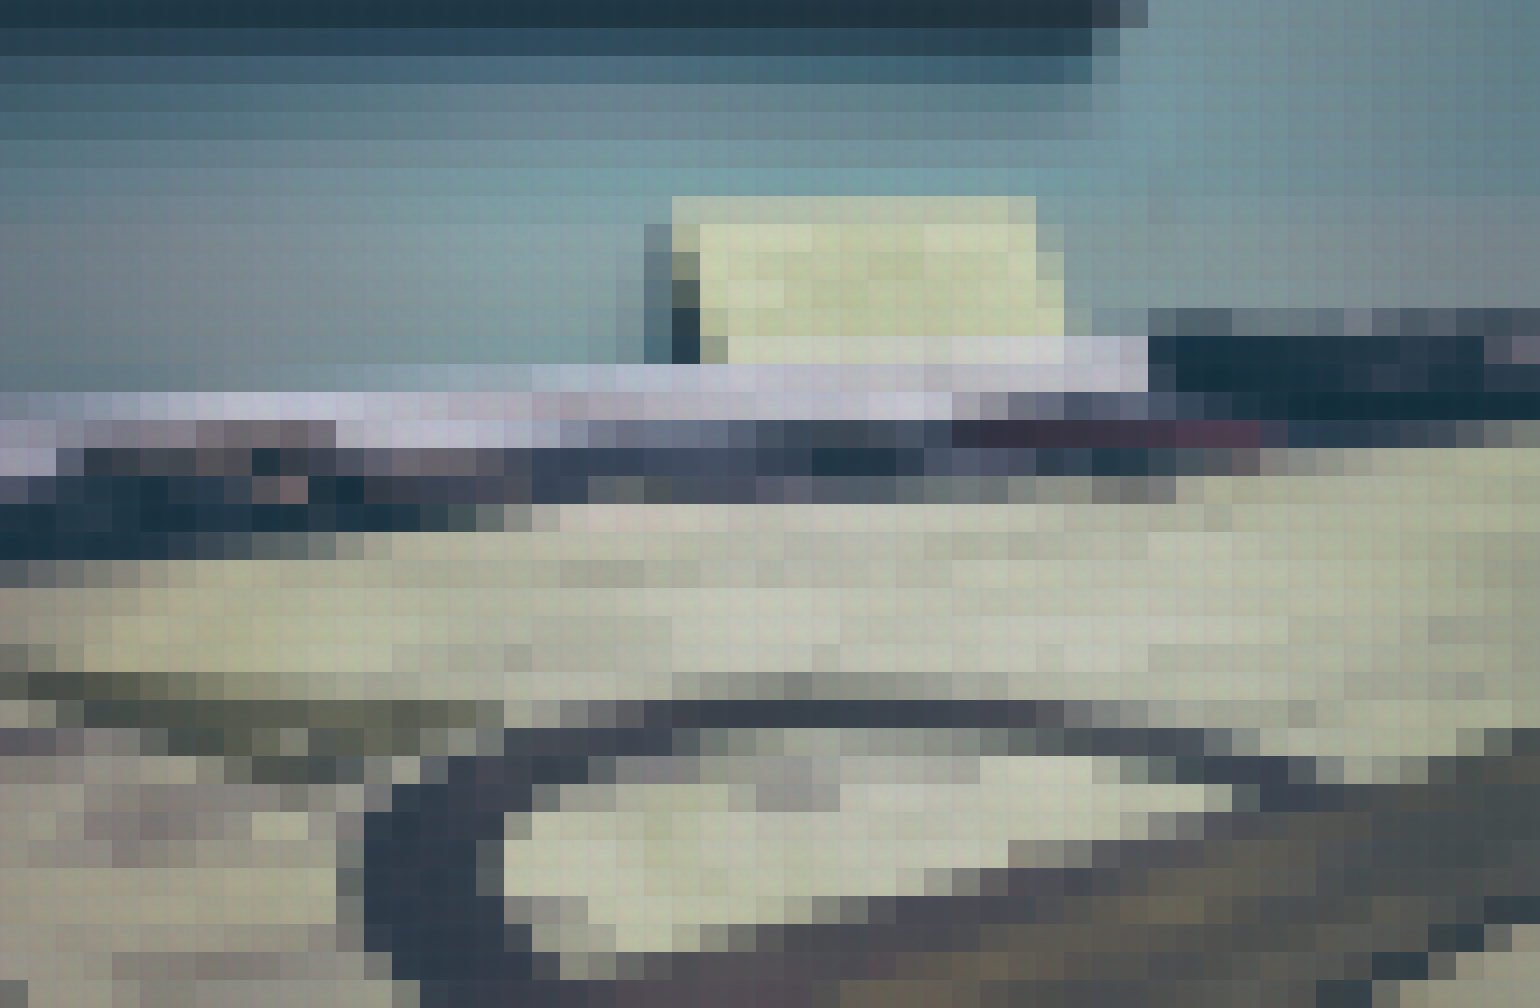
\includegraphics[width=\textwidth]{Images/autoencoder/reconstructed/512_256_128/test3_80.png}
    \subcaption{(512, 256, 128)}
    \end{subfigure}
    \caption{Output of auto-encoder width different number of hidden layers, $s=80$, epochs=$30$.}
    \label{fig:auto_layers}
\end{figure}

Since the sigmoid function (as well as the tanh function) cause vanishing gradients during backpropagation for networks with multiple layers, it was replaced by the ReLU function for all layers. Since ReLU is piecewise linear, we avoid the vanishing gradient problem and the network learns faster and performs better. Using the three-layer architecture and ReLU as an activation function, we obtain results which are shown in Figure \ref{fig:auto_relu}. With this setup, a lot more details are preserved and we don't obtain the strong aliasing effects as before. However, a repetitive pattern is observable in the reconstruction of all three test images. \\

\begin{figure}
    \centering
    \begin{subfigure}[b]{0.7 \textwidth}
    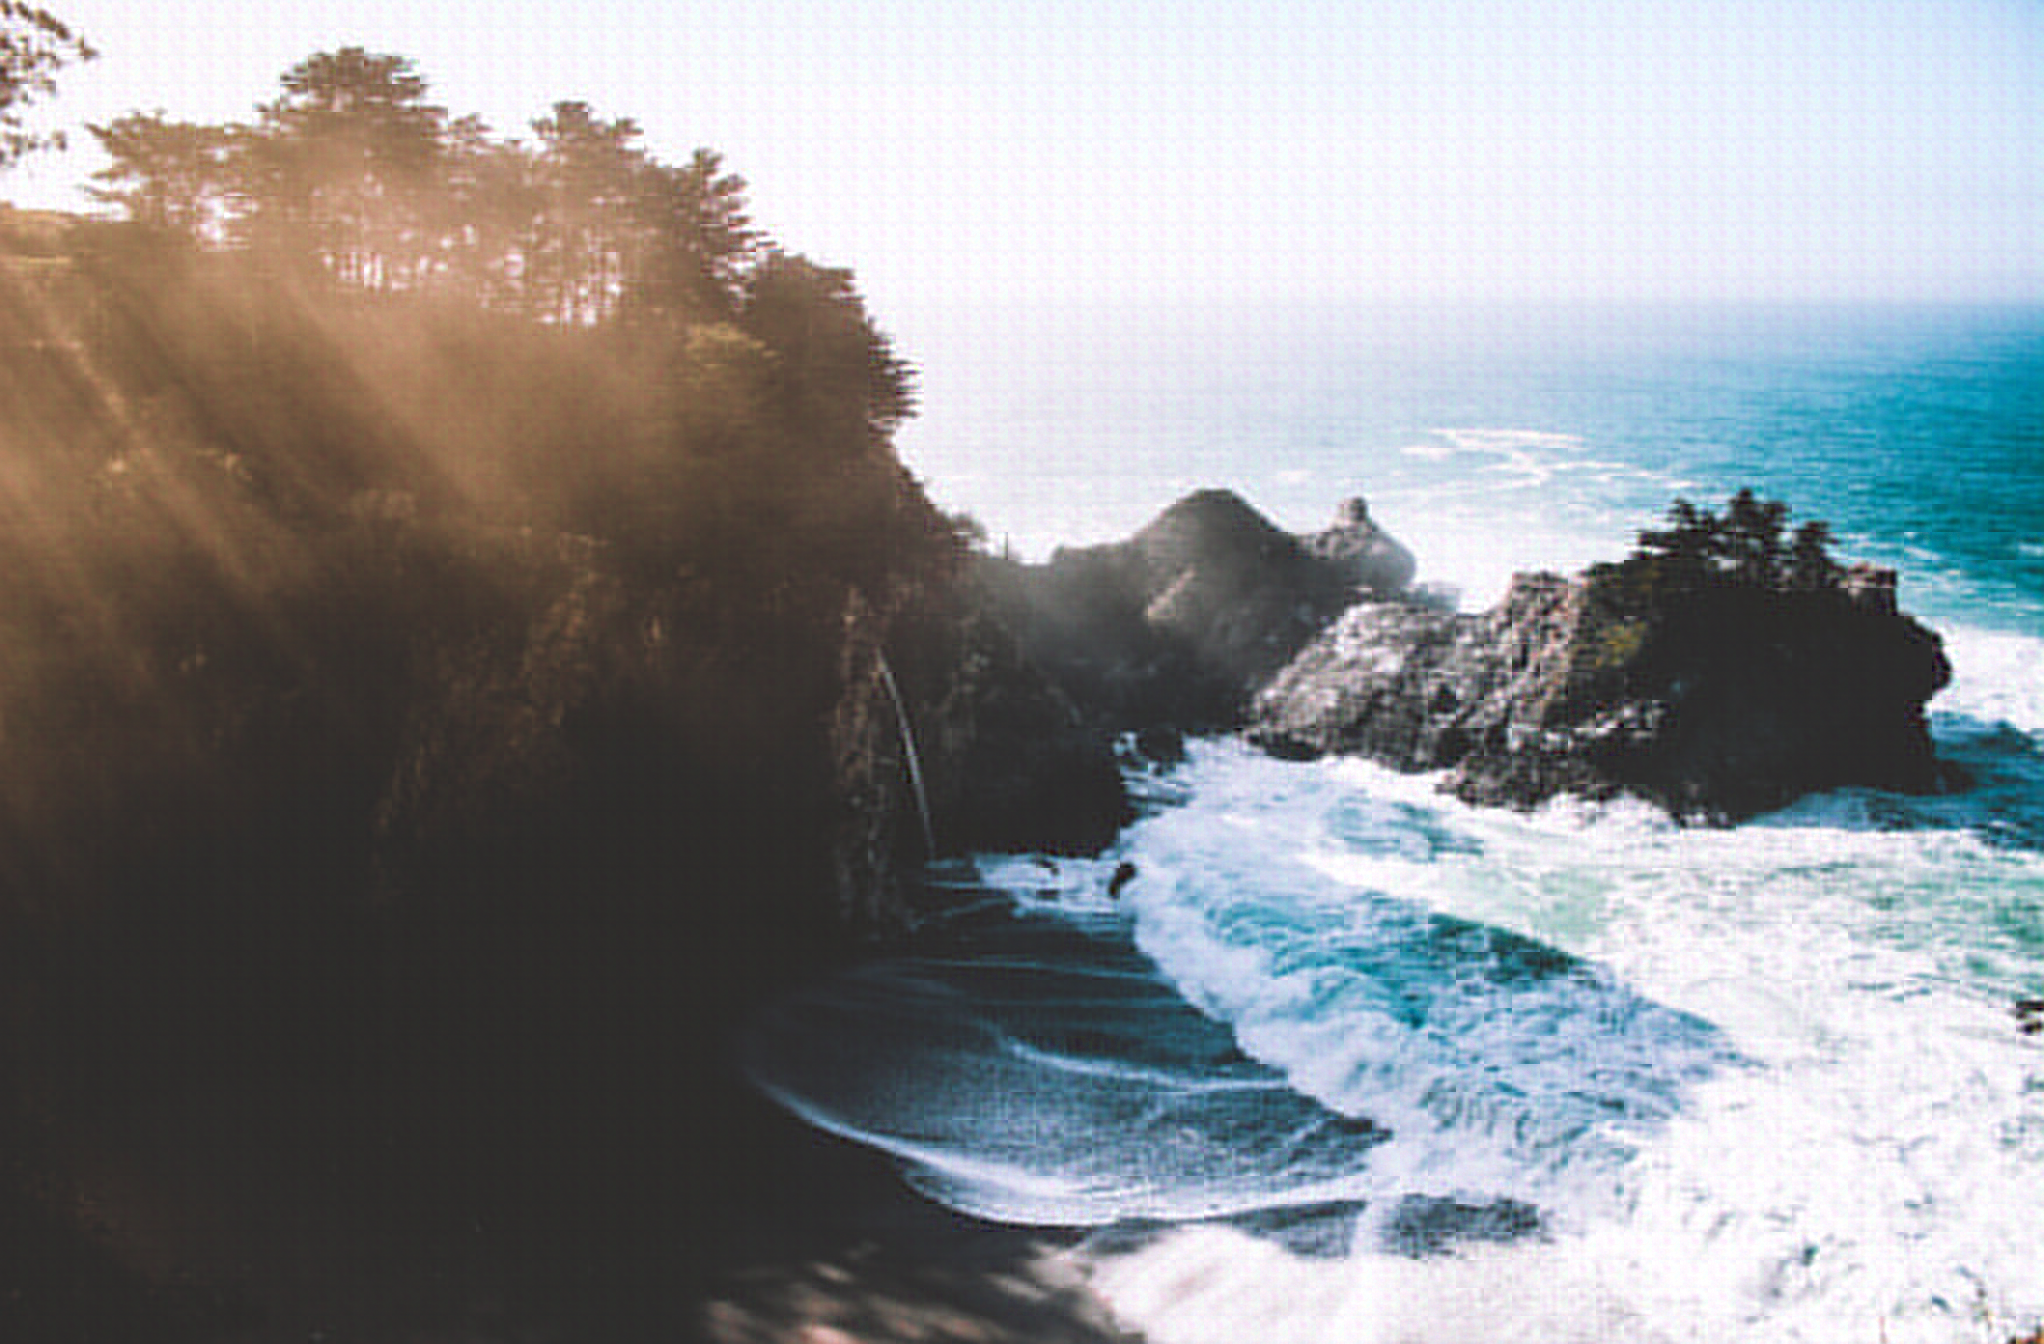
\includegraphics[width=\textwidth]{Images/autoencoder/reconstructed/512_256_128/test1_80_relu.png}
    \end{subfigure}
    \begin{subfigure}[b]{0.7 \textwidth}
    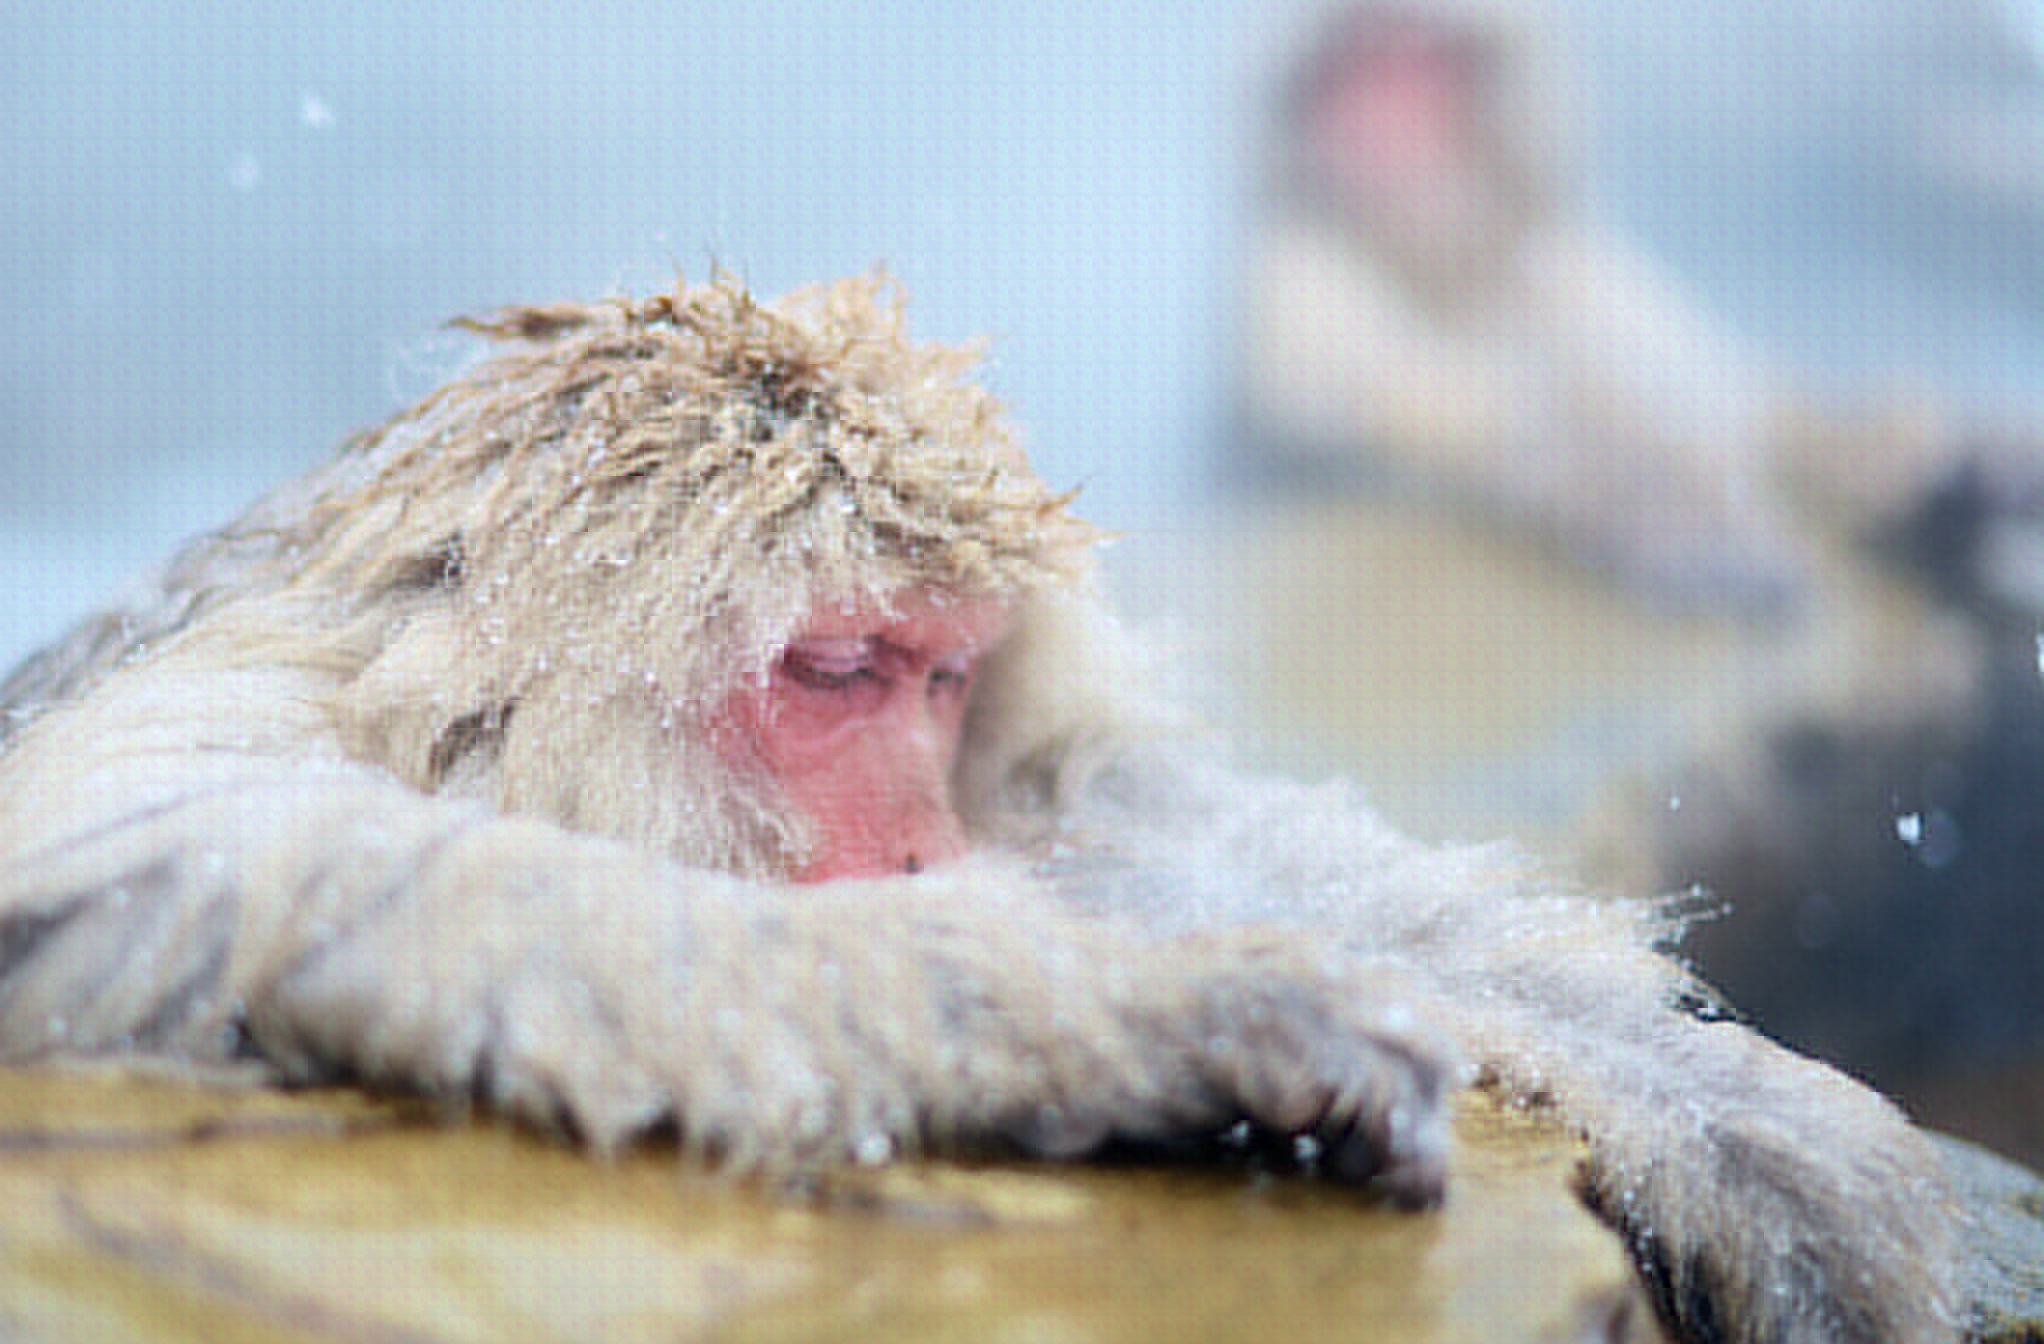
\includegraphics[width=\textwidth]{Images/autoencoder/reconstructed/512_256_128/test2_80_relu.png}
    \end{subfigure}
    \begin{subfigure}[b]{0.7 \textwidth}
    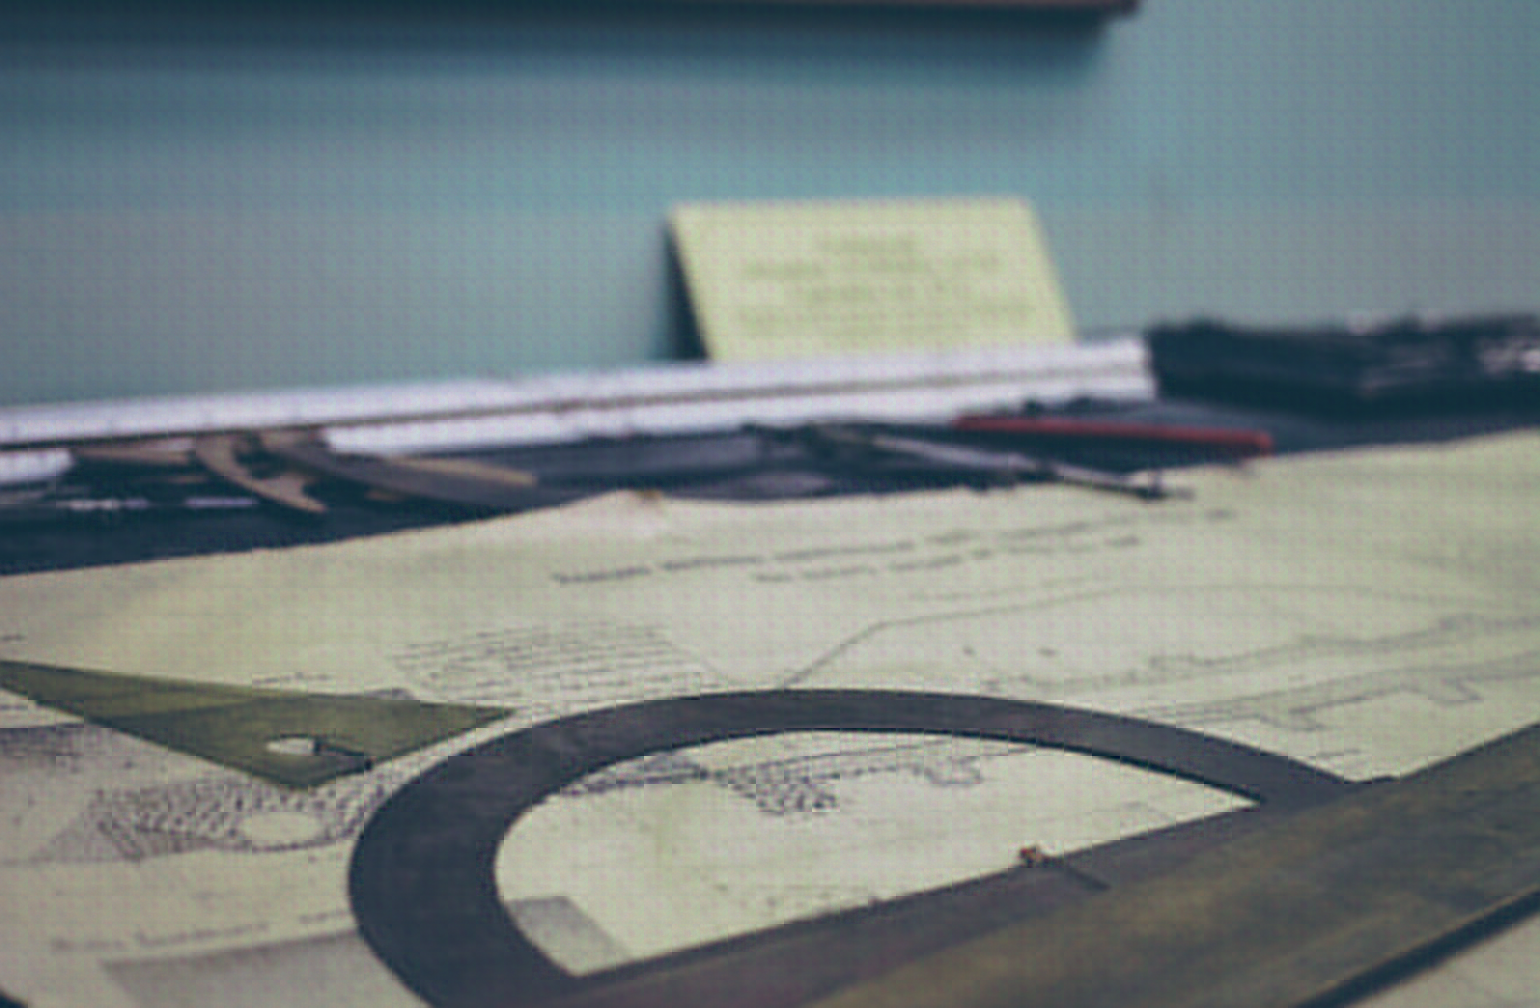
\includegraphics[width=\textwidth]{Images/autoencoder/reconstructed/512_256_128/test3_80_relu.png}
    \end{subfigure}
    \caption{Three-layer architecture with ReLU as activation function.}
    \label{fig:auto_relu}
\end{figure}


Last but not least, the learning rate was reduced by a factor of $10$, i.e. it became $5 \cdot 10^{-5}$. A low learning rate leads to slower convergence. However, having a (too) large learning rate can lead to the effect of not reaching the optimum or actually diverging from it. With the slower convergence, the number of epochs had to be increased a lot, i.e. it was set to $100$. As expected this lead to longer computation times. We can observe in Figure \ref{fig:auto_lr}, that this setup reduces the strong pattern effects which we had before and produces results which start to be comparable to the JPEG compression.

\begin{figure}
    \centering
    \begin{subfigure}[b]{0.7 \textwidth}
    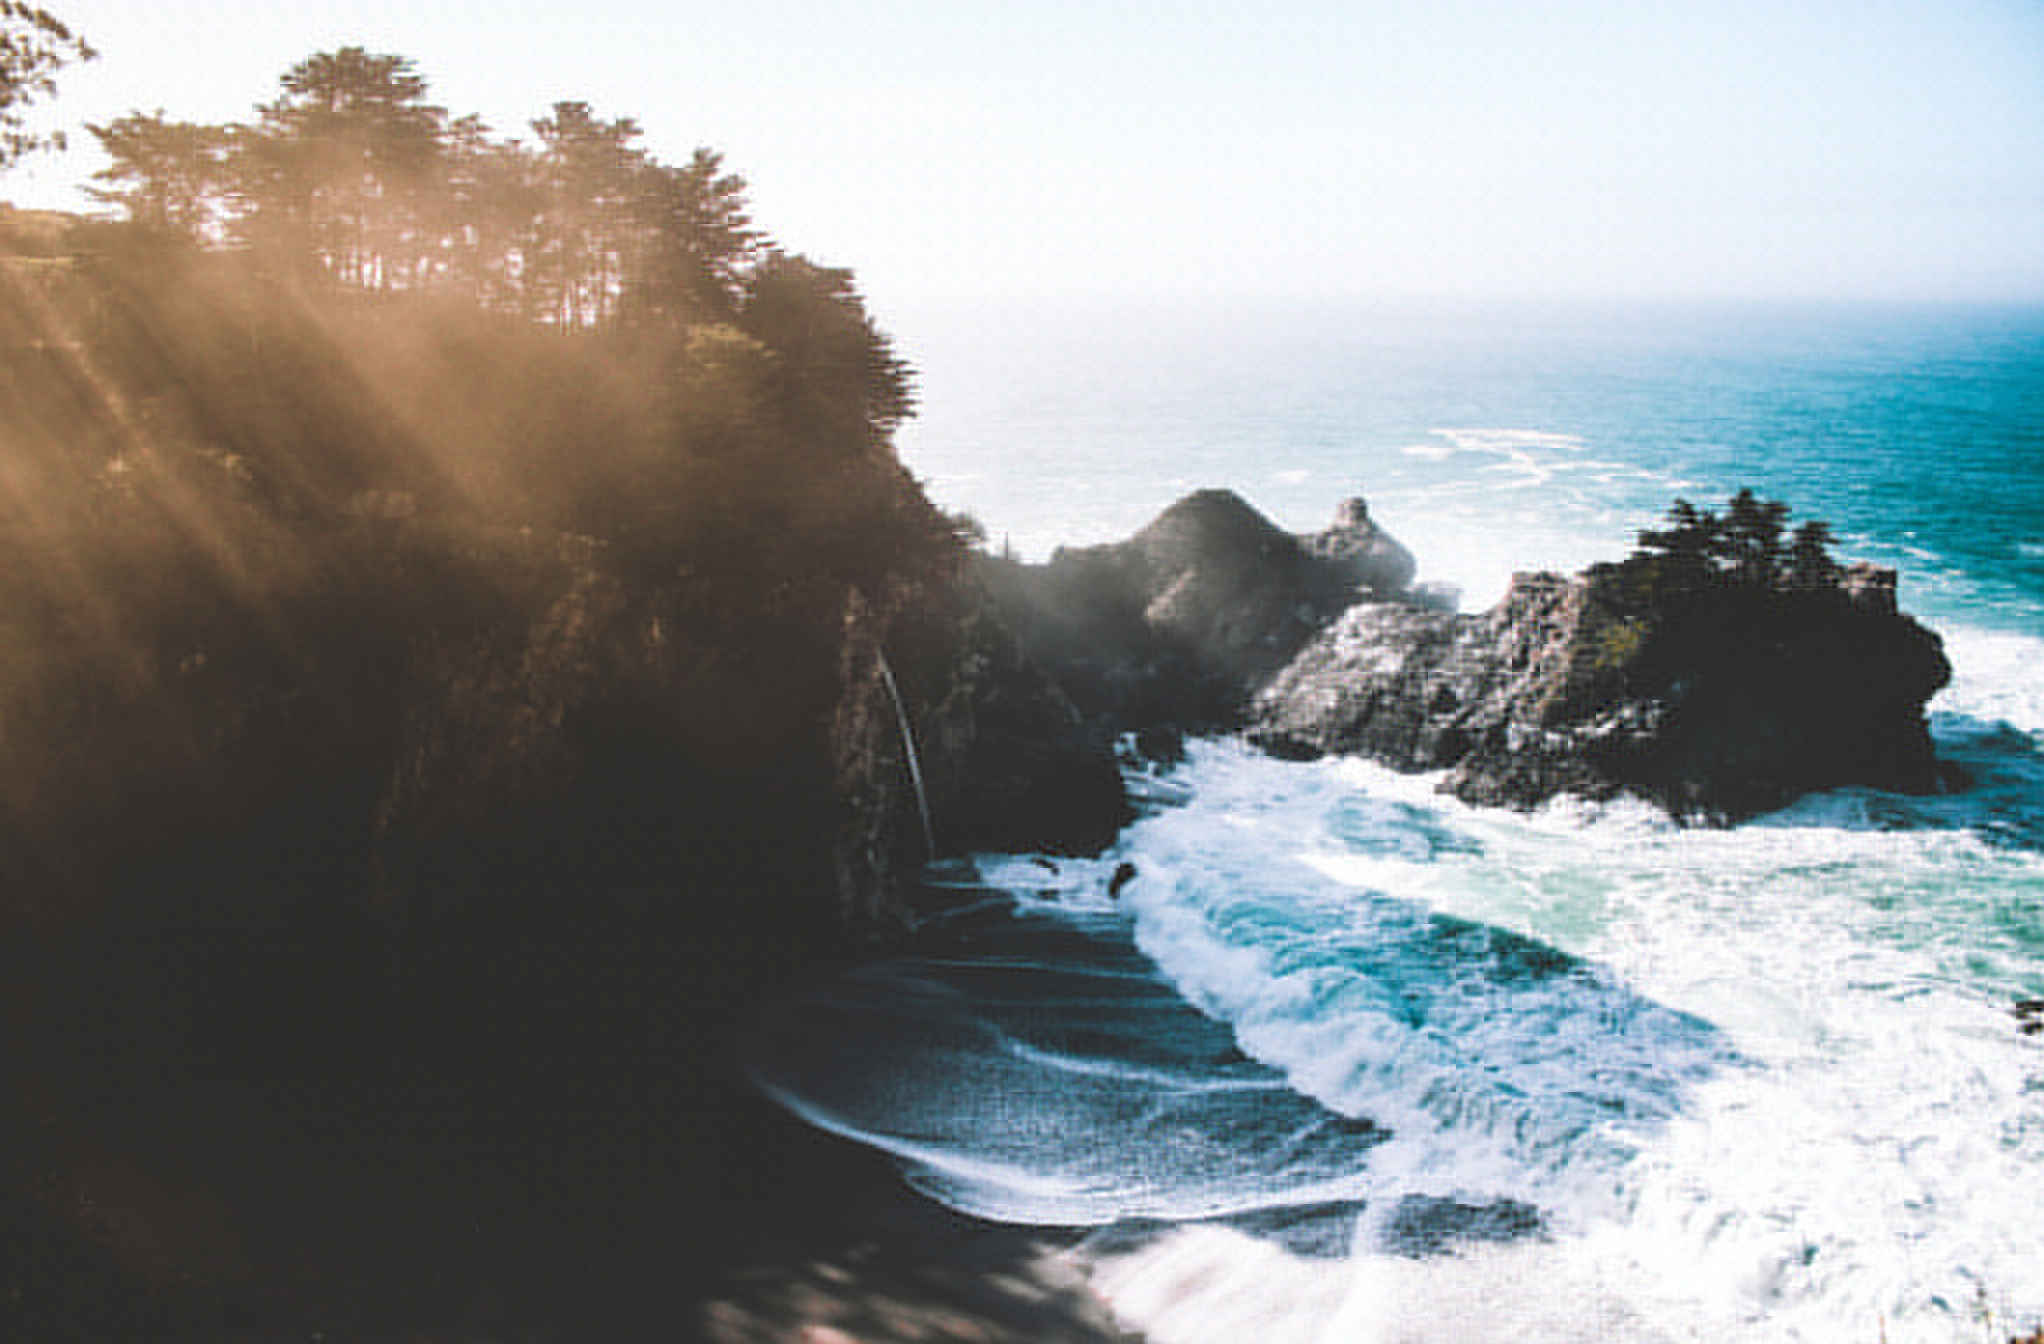
\includegraphics[width=\textwidth]{Images/autoencoder/reconstructed/512_256_128/lr/test1_80.png}
    \end{subfigure}
    \begin{subfigure}[b]{0.7 \textwidth}
       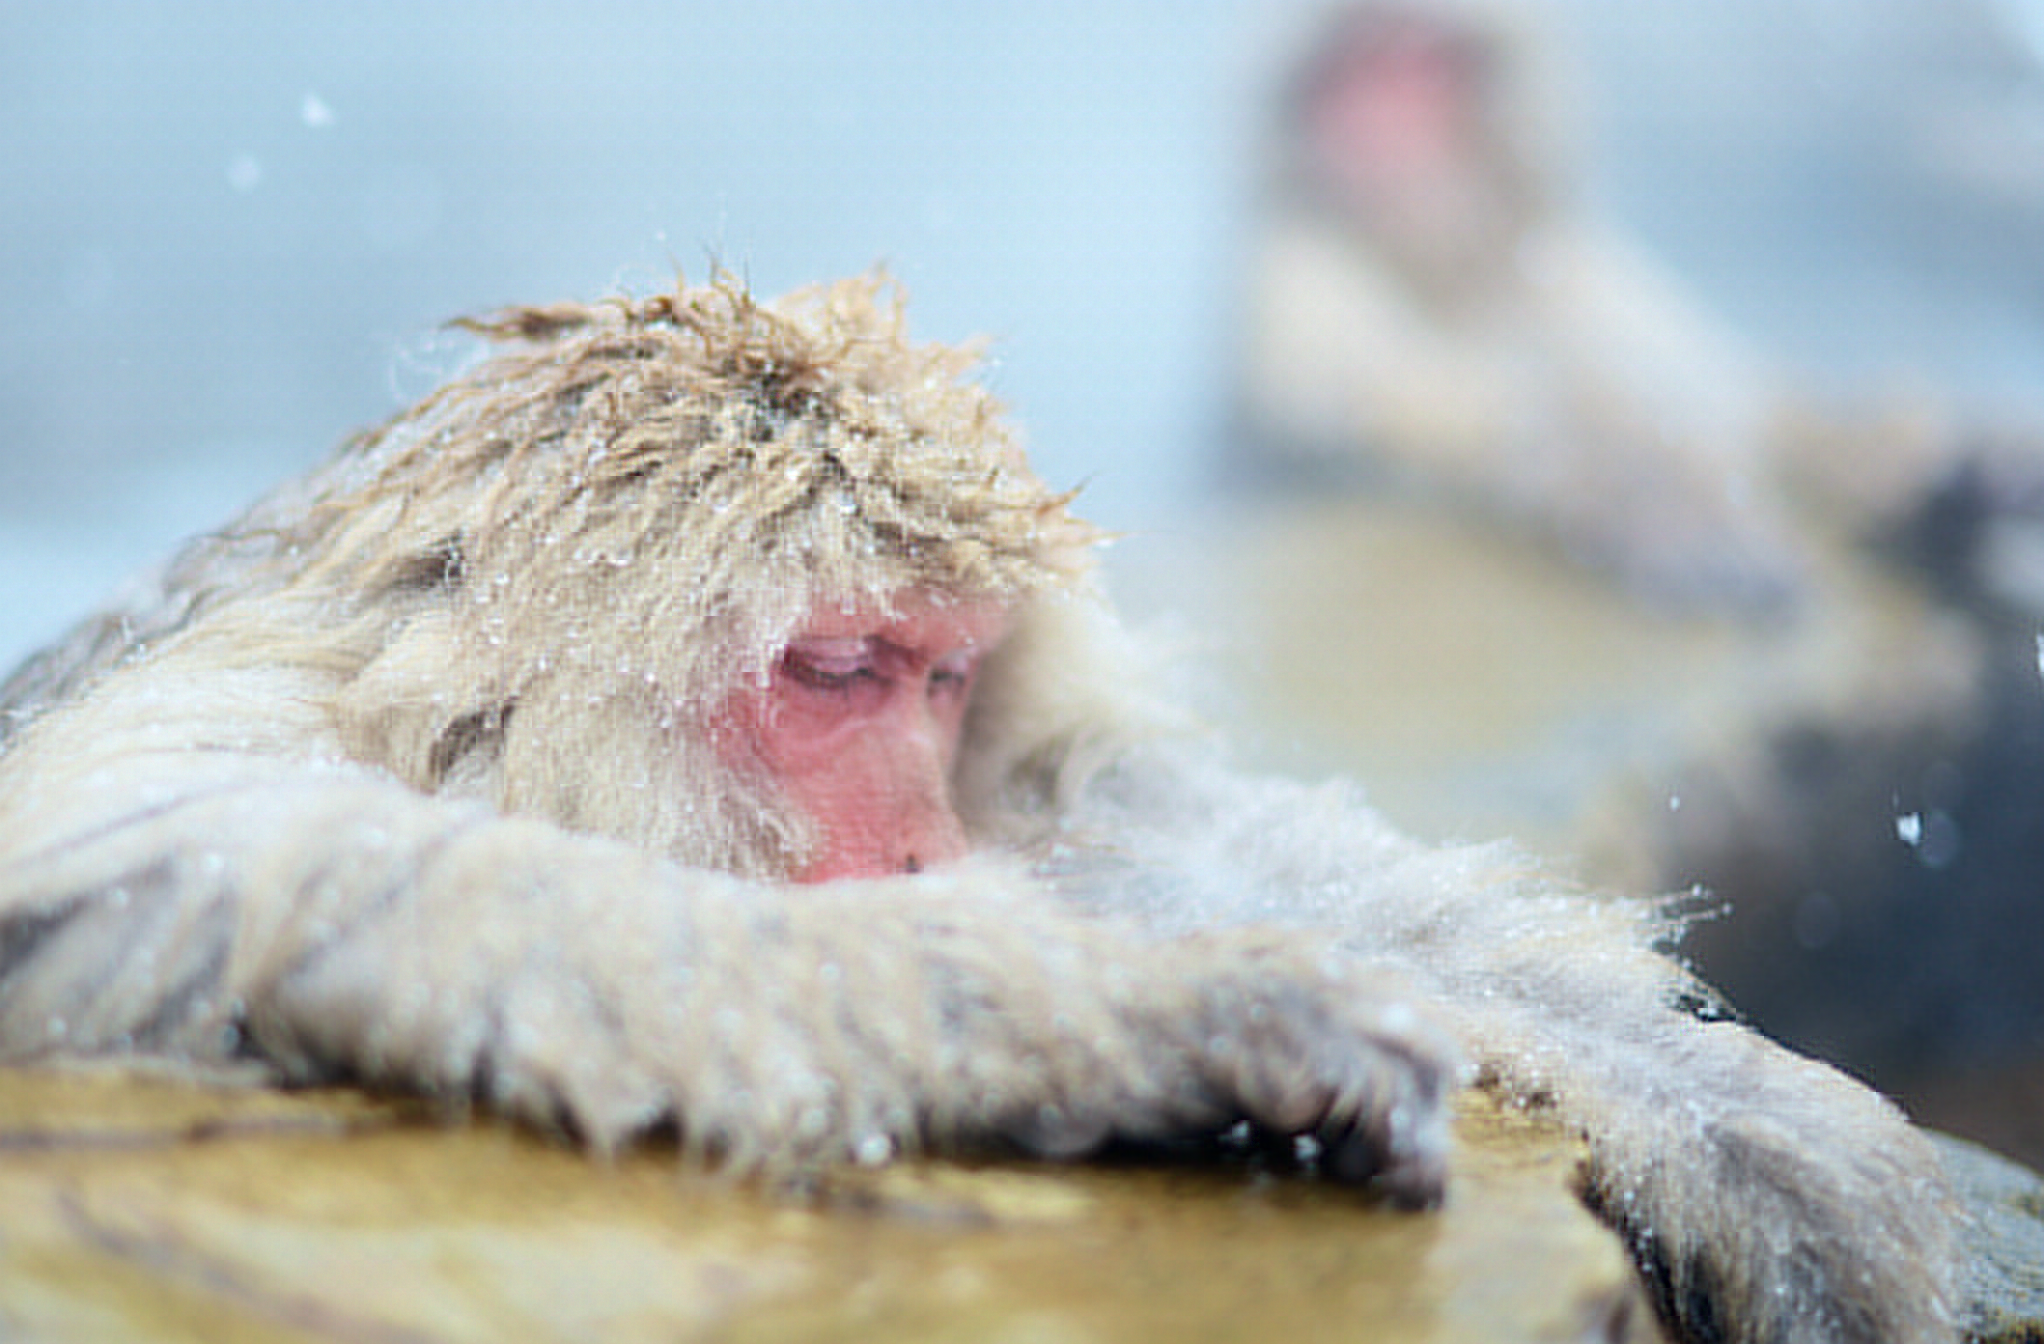
\includegraphics[width=\textwidth]{Images/autoencoder/reconstructed/512_256_128/lr/test2_80.png}
    \end{subfigure}
    \begin{subfigure}[b]{0.7 \textwidth}
     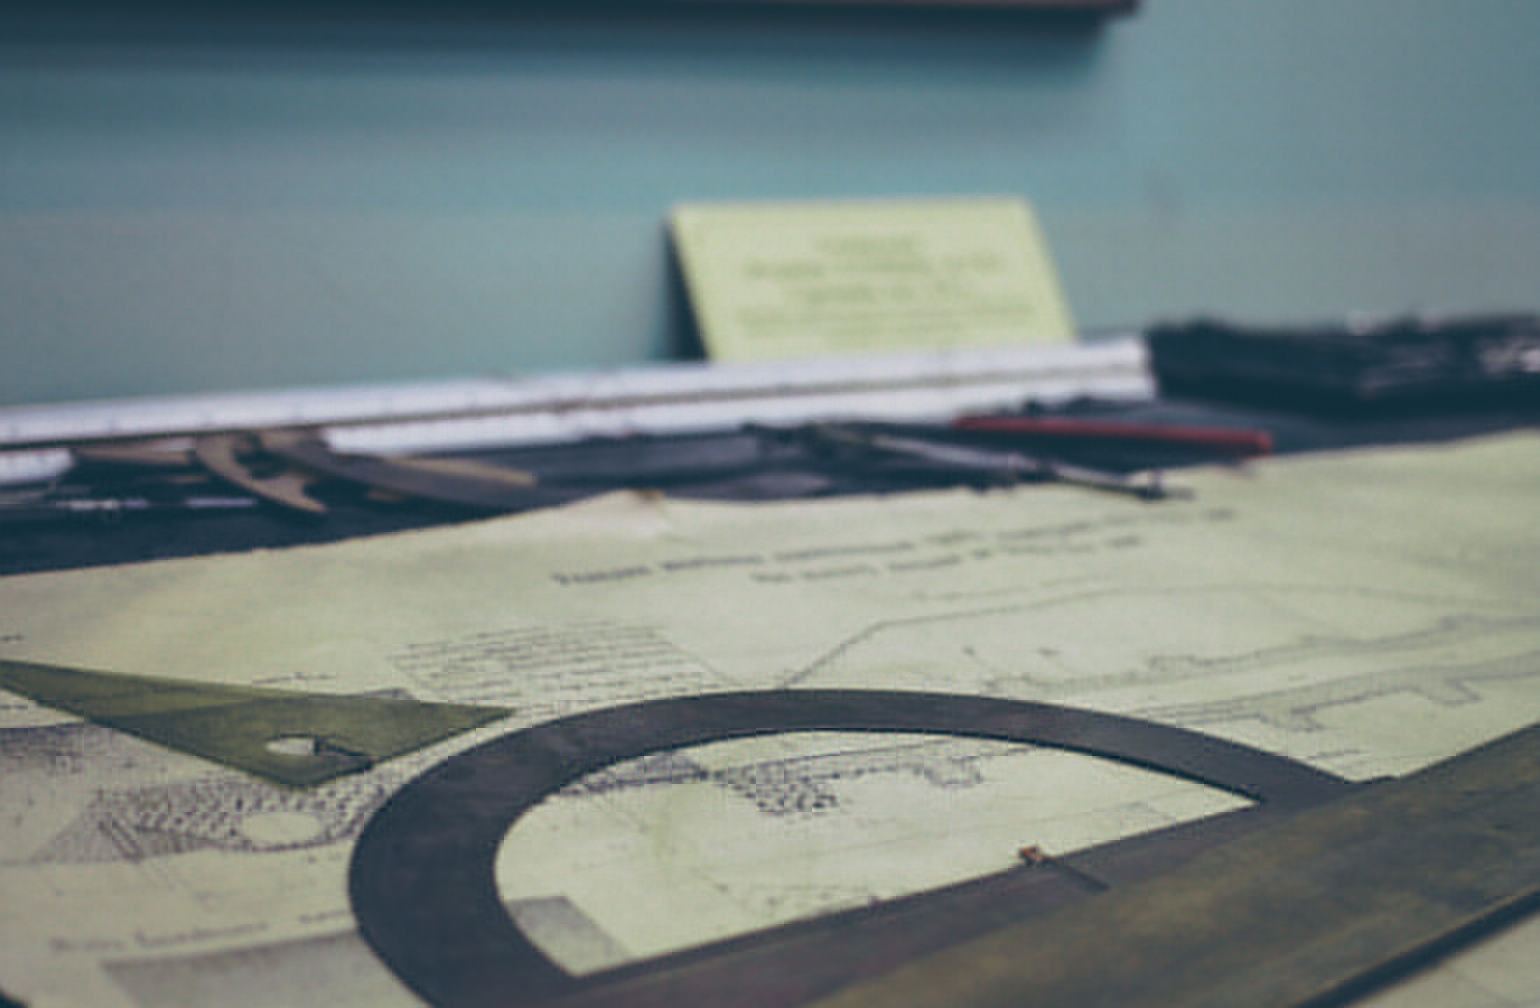
\includegraphics[width=\textwidth]{Images/autoencoder/reconstructed/512_256_128/lr/test3_80.png}
    \end{subfigure}
    \caption{Lowered learning rate ($5 \cdot 10^{-5}$) and increased number of epochs ($100$).}
    \label{fig:auto_lr}
\end{figure}

%---------------------------
% Task 3
%---------------------------
\section{Objective Evaluation}
In this exercise, we were asked to evaluate the quality of the two compression approaches using the objective quality metrics PSNR, SSIM, MSSIM and VIF. In the case of JPEG, the objective quality metrics were computed for compressions with Q-values between $10$ and $90$ (step size of $10$). For the auto-encoder compression, the objective quality metrics were computed for latent sizes between $10$ and $70$. Figure \ref{fig:objective_PSNR} plots PSNR against the bits per pixel (bpp) for JPEG (blue) and the auto-encoder (red). Figure \ref{fig:objective_SSIM} follows the same pattern but plotting SSIM against bpp, Figure \ref{fig:objective_MSSIM} showing the MSSIM and Figure \ref{fig:objective_VIF} the VIF values. In order to compare the objective metric values between the JPEG and the auto-encoder compression reasonably, we shall only look at metric values in the same bpp range. For JPEG, this corresponds to Q being between $80$ and $90$. For the auto-encoder, a network with latent size $s=10$ or $s=20$ falls into this overlapping range. \\

Looking at the plots, we can observe that in the region of interest, i.e. where the JPEG and auto-encoder bpp values overlap, the JEPG compression always introduces higher metric values according to the four metrics used on all test images. Note that the scaling  of the y-axis might vary between the different test images. For example, for test image \textsf{test2.png}, the quality between JPEG and and the auto-encoder is closer to each other according to all four objective quality metrics. \\

For all four metrics, higher values generally indicate that the reconstruction is of higher quality. Since all four metrics indicate the same results on all test images, one can conclude that the JPEG compression leads to better results according to the objective quality metrics. Since some metrics incorporate different possible error sources such as different distances from the screen (MS-SSIM), better modeling the perception of th HVS (SSIM), etc., one can say that these results are representative.

\begin{figure}
    \centering
    \begin{subfigure}[b]{0.7 \textwidth}
    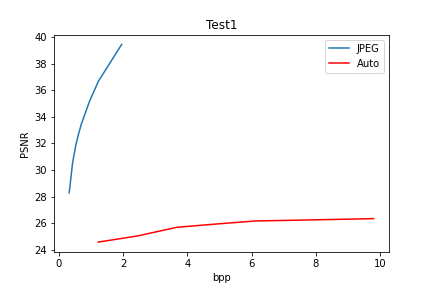
\includegraphics[width=\textwidth]{Images/Plots/test1_PSNR.png}
    \end{subfigure}
    \begin{subfigure}[b]{0.7 \textwidth}
    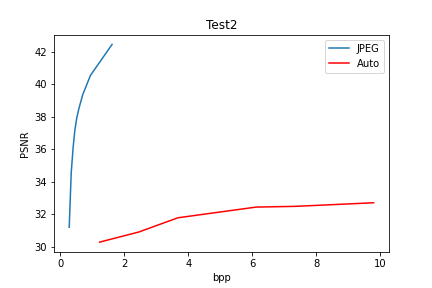
\includegraphics[width=\textwidth]{Images/Plots/test2_PSNR.png}
    \end{subfigure}
    \begin{subfigure}[b]{0.7 \textwidth}
    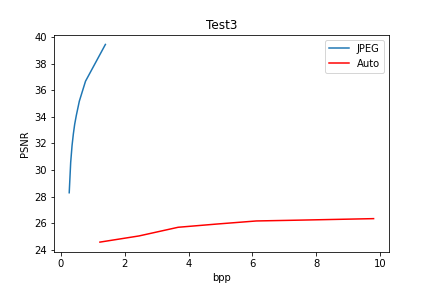
\includegraphics[width=\textwidth]{Images/Plots/test3_PSNR.png}
    \end{subfigure}
    \caption{PSNR against bpp for all test images.}
    \label{fig:objective_PSNR}
\end{figure}

\begin{figure}
    \centering
    \begin{subfigure}[b]{0.7 \textwidth}
    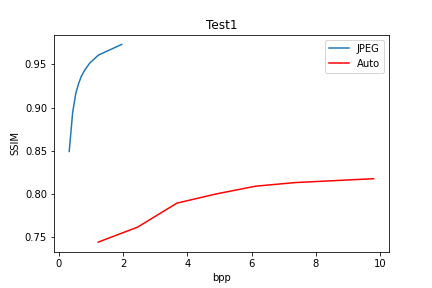
\includegraphics[width=\textwidth]{Images/Plots/test1_SSIM.png}
    \end{subfigure}
    \begin{subfigure}[b]{0.7 \textwidth}
    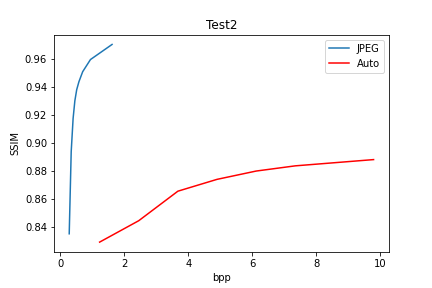
\includegraphics[width=\textwidth]{Images/Plots/test2_SSIM.png}
    \end{subfigure}
    \begin{subfigure}[b]{0.7 \textwidth}
    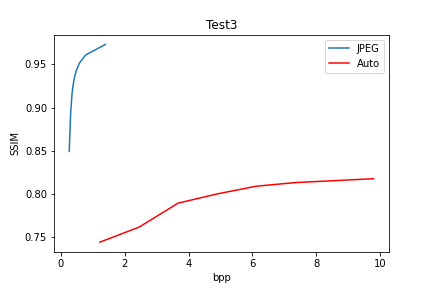
\includegraphics[width=\textwidth]{Images/Plots/test3_SSIM.png}
    \end{subfigure}
    \caption{SSIM against bpp for all test images.}
    \label{fig:objective_SSIM}
\end{figure}



\begin{figure}
    \centering
    \begin{subfigure}[b]{0.7 \textwidth}
    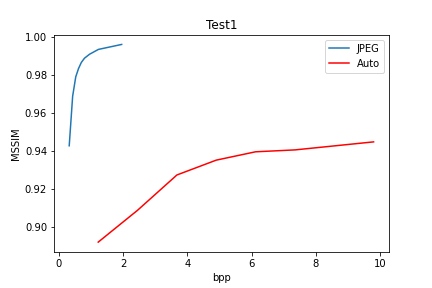
\includegraphics[width=\textwidth]{Images/Plots/test1_MSSIM.png}
    \end{subfigure}
    \begin{subfigure}[b]{0.7 \textwidth}
    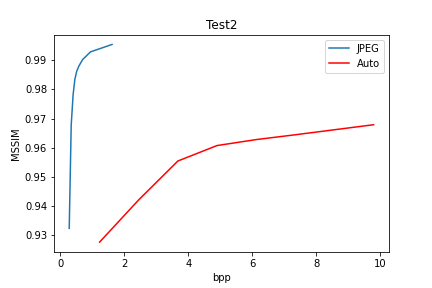
\includegraphics[width=\textwidth]{Images/Plots/test2_MSSIM.png}
    \end{subfigure}
    \begin{subfigure}[b]{0.7 \textwidth}
    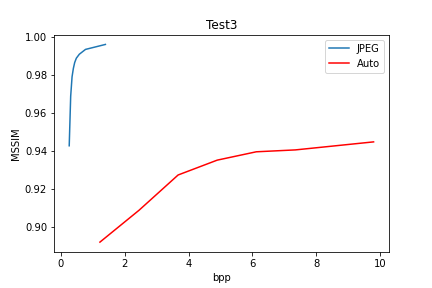
\includegraphics[width=\textwidth]{Images/Plots/test3_MSSIM.png}
    \end{subfigure}
    \caption{MSSIM against bpp for all test images.}
    \label{fig:objective_MSSIM}
\end{figure}


\begin{figure}
    \centering
    \begin{subfigure}[b]{0.7 \textwidth}
    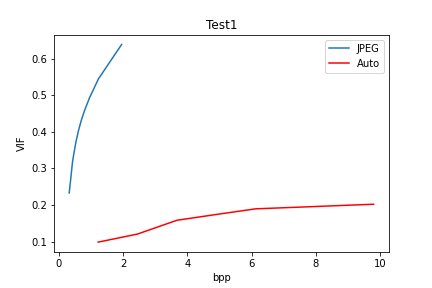
\includegraphics[width=\textwidth]{Images/Plots/test1_VIF.png}
    \end{subfigure}
    \begin{subfigure}[b]{0.7 \textwidth}
    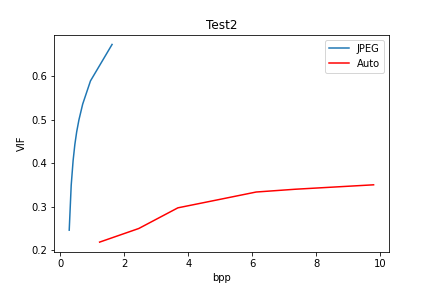
\includegraphics[width=\textwidth]{Images/Plots/test2_VIF.png}
    \end{subfigure}
    \begin{subfigure}[b]{0.7 \textwidth}
    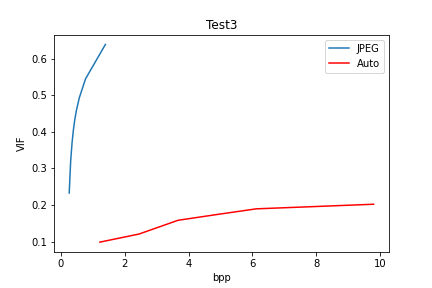
\includegraphics[width=\textwidth]{Images/Plots/test3_VIF.png}
    \end{subfigure}
    \caption{VIF against bpp for all test images.}
    \label{fig:objective_VIF}
\end{figure}




%---------------------------
% Task 4
%---------------------------
\section{Subjective Evaluation}

As already briefly mentioned in Section 2, the finally chosen auto-encoder ((512, 256, 128), ReLU, $lr = 5 \cdot 10^{-5}$, $100$ epochs) leads to reconstructed results which are close to the original when being viewed from approx. $50cm$ away from the screen. However, if you zoom into the image or move closer to the screen, you might observe the repeating patterns which could also be observed in previous auto-encoder versions (however, there they were a lot more dominant). Those repeating patterns also introduce slight aliasing artefacts at the contours of objects. We could also observe aliasing artefacts in JPEG compression with a low Q-value. However, they were not introduced through repeating patterns but more through larger areas consisting of the same color which also lead to false contours.\\

These subjective results, i.e. that the JPEG compression produces better visual results in the reconstruction, also correspond to the results observed in the objective quality assessment. \\

In terms of compression efficiency, one can say that JPEG is also more efficient. For the auto-encoder, we obtain the best visual results for a latent size of $s=80$. This corresponds to a bpp value of approx. $9.79$. In contrast, for JEPG compression we already achieve good results for $Q=50$, which corresponds to a bpp value between $0.43$ and $0.6$ depending on the input image. Thus, JPEG is also a lot more efficient. \\

To conclude, let's now summarize how the different hyperparameters influenced the performance of the auto-encoder compression:
\begin{itemize}
    \item Latent size $s$: the larger the latent space, the better the transition between adjacent pattern elements.
    \item Depth of network: the deeper the auto-encoder, the better the compression if the correct activation function is used. Furthermore, deeper networks often require less training data to learn a task. However, this was not investigated in this assignment.
    \item Activation function: for deeper networks, we have to use ReLu as an activation function to avoid vanishing gradients. This strongly improves the visual quality of the deeper auto-encoder.
    \item Learning rate: the smaller the learning rate, the slower the convergence to the optimum and thus more epochs are needed for training. However, small learning rates ensure that we reach the optimum and don't diverge.
\end{itemize}

Last but not least, it is worth mentioning that the performance of the auto-encoder could be further improved by replacing the linear layers through convolutional layers. With such layers, the network can learn highly specific features on different levels which can be detected anywhere on test images.
\end{document}